% **************************************************************************************************************
% A Classic Thesis Style
% An Homage to The Elements of Typographic Style
% **************************************************************************************************************
\RequirePackage{silence}
    \WarningFilter{scrreprt}{Usage of package `titlesec'}
    %\WarningFilter{scrreprt}{Activating an ugly workaround}
    \WarningFilter{titlesec}{Non standard sectioning command}
\documentclass[ %twoside,openright,
titlepage,numbers=noenddot,%1headlines,
                headinclude,footinclude,cleardoublepage=empty,abstract=on,
                BCOR=5mm,paper=a4,fontsize=11pt
                ]{scrreprt}

%********************************************************************
% Note: Make all your adjustments in here
%*******************************************************
% ****************************************************************************************************

% ****************************************************************************************************
% 0. Set the encoding of your files. UTF-8 is the only sensible encoding nowadays. If you can't read
% äöüßáéçèê∂åëæƒÏ€ then change the encoding setting in your editor, not the line below. If your editor
% does not support utf8 use another editor!
% ****************************************************************************************************
\usepackage{fontspec}
% \PassOptionsToPackage{utf8}{inputenc}
%   \usepackage{inputenc}

% \PassOptionsToPackage{T1}{fontenc} % T2A for cyrillics
%   \usepackage{fontenc}

% this solves a warning about bullet points
\usepackage{textcomp}
% \usepackage{titling}

% ****************************************************************************************************
% 1. Configure classicthesis for your needs here, e.g., remove "drafting" below
% in order to deactivate the time-stamp on the pages
% (see ClassicThesis.pdf for more information):
% ****************************************************************************************************
\PassOptionsToPackage{
  drafting=false,    % print version information on the bottom of the pages
  tocaligned=false, % the left column of the toc will be aligned (no indentation)
  dottedtoc=true,  % page numbers in ToC flushed right
  eulerchapternumbers=true, % use AMS Euler for chapter font (otherwise Palatino)
  linedheaders=true,       % chapter headers will have line above and beneath
  floatperchapter=true,     % numbering per chapter for all floats (i.e., Figure 1.1)
  eulermath=true,  % use awesome Euler fonts for mathematical formulae (only with pdfLaTeX)
  beramono=true,    % toggle a nice monospaced font (w/ bold)
  palatino=false,    % deactivate standard font for loading another one, see the last section at the end of this file for suggestions
  parts=true,
  style=classicthesis % classicthesis, arsclassica
  % style=arsclassica % classicthesis, arsclassica
}{classicthesis}


% ****************************************************************************************************
% 2. Personal data and user ad-hoc commands (insert your own data here)
% ****************************************************************************************************
\newcommand{\myTitle}{Semi-supervised Methods for Distributionally-Robust Learning}
% \newcommand{\mySubtitle}{\xspace}
\newcommand{\myDegree}{A thesis submitted for the degree of Doctor of Philosophy.\xspace}
\newcommand{\myName}{Myles Bartlett \xspace}
% \newcommand{\myProf}{Put name here\xspace}
% \newcommand{\myOtherProf}{Put name here\xspace}
% \newcommand{\mySupervisor}{Put name here\xspace}
\newcommand{\myFaculty}{School of Engineering and Informatics\xspace}
% \newcommand{\myDepartment}{Put data here\xspace}
\newcommand{\myUni}{University of Sussex\xspace}
\newcommand{\myLocation}{Brighton\xspace}
\newcommand{\myTime}{April 2023\xspace}
\newcommand{\myVersion}{Thesis v1.1-rc1}

% ********************************************************************
% Setup, finetuning, and useful commands
% ********************************************************************
\providecommand{\mLyX}{L\kern-.1667em\lower.25em\hbox{Y}\kern-.125emX\@}
\newcommand{\ie}{i.\,e.}
\newcommand{\Ie}{I.\,e.}
\newcommand{\eg}{e.\,g.}
\newcommand{\Eg}{E.\,g.}
% ****************************************************************************************************


% ****************************************************************************************************
% 3. Loading some handy packages
% ****************************************************************************************************
% ********************************************************************
% Packages with options that might require adjustments
% ********************************************************************
\usepackage{polyglossia}
\setdefaultlanguage[variant=british]{english}

\PassOptionsToPackage{hyphens}{url}
\usepackage{csquotes}
\PassOptionsToPackage{%
  backend=biber,bibencoding=utf8, %instead of bibtex
  % backend=bibtex8,bibencoding=ascii,%
  language=british,%
  %style=numeric-comp,%
  %bibstyle=authoryear,dashed=false, % dashed: substitute rep. author with ---
  sorting=ynt, % name, year, title
  uniquelist=false,
  maxbibnames=8, % default: 3, et al.
  maxcitenames=2,
  mincitenames=1,
  style=authoryear-comp, % Author 1999, 2010
  %backref=true,%
  uniquename=false,  % suppresses initials for authors with same last name
  natbib=true % natbib compatibility mode (\citep and \citet still work)
}{biblatex}
    \usepackage{biblatex}

\defbibenvironment{bibwithnumlabel}
  {\list
    {\printfield[labelnumberwidth]{labelnumber}}
    {\setlength{\labelwidth}{\labelnumberwidth}%
    \setlength{\leftmargin}{\labelwidth}%
    \setlength{\labelsep}{\biblabelsep}%
    \addtolength{\leftmargin}{\labelsep}%
    \setlength{\itemsep}{\bibitemsep}%
    \setlength{\parsep}{\bibparsep}}%
    \renewcommand*{\makelabel}[1]{\hss##1}}
  {\endlist}
  {\item}

\usepackage{amsmath}
\usepackage{amssymb}
\usepackage{import}
\usepackage{colortbl}
  
% ********************************************************************
% General useful packages
% ********************************************************************
\usepackage{graphicx} %
\usepackage{scrhack} % fix warnings when using KOMA with listings package
\usepackage{xspace} % to get the spacing after macros right
\PassOptionsToPackage{printonlyused,smaller}{allacronym}
  \usepackage{acronym} % nice macros for handling all acronyms in the thesis
  %\renewcommand{\bflabel}[1]{{#1}\hfill} % fix the list of acronyms --> no longer working
  %\renewcommand*{\acsfont}[1]{\textsc{#1}}
  %\renewcommand*{\aclabelfont}[1]{\acsfont{#1}}
  %\def\bflabel#1{{#1\hfill}}
  \def\bflabel#1{{\acsfont{#1}\hfill}}
  \def\aclabelfont#1{\acsfont{#1}}
% \usepackage{glossaries}
% \input{glossary.tex}

% ************** %
%  Nomenclature  %
% ************** %
\newlength{\nomenlabelindent}
\setlength{\nomenlabelindent}{2em}
\newenvironment{nomenclature}{%
\newcommand\entry[2]{%
\hangindent\nomenlabelindent\noindent\makebox[\nomenlabelindent][l]{##1\quad}\ignorespaces##2\par\addvspace{9pt}}%
   \chapter*{Nomenclature}}{\par\addvspace{12pt}}

% ************** %
%  Simple glossary  %
% ************** %
\newlength{\glossarylabelindent}
\setlength{\glossarylabelindent}{11em}
\newenvironment{glossaryenv}{%
\newcommand\entry[2]{%
\hangindent\glossarylabelindent\noindent\makebox[\glossarylabelindent][l]{\bfseries ##1\quad}\ignorespaces##2\par\addvspace{9pt}}%
   \chapter*{Glossary}}{\par\addvspace{12pt}}
% ****************************************************************************************************
%\usepackage{pgfplots} % External TikZ/PGF support (thanks to Andreas Nautsch)
%\usetikzlibrary{external}
%\tikzexternalize[mode=list and make, prefix=ext-tikz/]
\usepackage[dvipsnames]{xcolor}
\usepackage[edges]{forest}
\usetikzlibrary{shadows.blur}
% ****************************************************************************************************


% ****************************************************************************************************
% 4. Setup floats: tables, (sub)figures, and captions
% ****************************************************************************************************
% \usepackage{booktabs} % better tables
  % \setlength{\extrarowheight}{3pt} % increase table row height
% \newcommand{\tableheadline}[1]{\multicolumn{1}{l}{\spacedlowsmallcaps{#1}}}
% \newcommand{\myfloatalign}{\centering} % to be used with each float for alignment
\usepackage{subcaption}
\usepackage[rightcaption]{sidecap} % <-- added
% Undo the hanging-caption format imposed by classicthesis
\captionsetup{format=plain, font=small, labelfont=bf}
% ****************************************************************************************************

% ****************************************************************************************************
% 5. Setup code listings
% ****************************************************************************************************
% \usepackage{listings}
% %\lstset{emph={trueIndex,root},emphstyle=\color{BlueViolet}}%\underbar} % for special keywords
% \lstset{language=[LaTeX]Tex,%C++,
%   morekeywords={PassOptionsToPackage,selectlanguage},
%   keywordstyle=\color{RoyalBlue},%\bfseries,
%   basicstyle=\small\ttfamily,
%   %identifierstyle=\color{NavyBlue},
%   commentstyle=\color{Green}\ttfamily,
%   stringstyle=\rmfamily,
%   numbers=none,%left,%
%   numberstyle=\scriptsize,%\tiny
%   stepnumber=5,
%   numbersep=8pt,
%   showstringspaces=false,
%   breaklines=true,
%   %frameround=ftff,
%   %frame=single,
%   belowcaptionskip=.75\baselineskip
%   %frame=L
% }
% ****************************************************************************************************




% ****************************************************************************************************
% 6. Last calls before the bar closes
% ****************************************************************************************************
\usepackage{classicthesis}
% for compatibility with Sussex requirements
% \usepackage[a4paper,top=2.5cm,bottom=2.5cm,left=4cm,right=2cm,headsep=10pt]{geometry}
% !!! for drafting, I'll use slightly incorrect margins, because it's annoying if the text isn't centered
\usepackage[a4paper,top=2.5cm,bottom=2.5cm,left=3cm,right=3cm,headsep=10pt]{geometry}
% \setmainfont[Ligatures=TeX,Numbers=OldStyle]{TeX Gyre Pagella} % Palatino clone
\linespread{1.05} % a bit more for Palatino
% \setmainfont[Ligatures=TeX,Numbers=OldStyle]{Linux Libertine O}
\setmainfont[Ligatures=TeX]{Libertinus Serif} % fork of Linux Libertine O
% \usepackage{unicode-math}
% \setmathfont{Libertinus Math}
% \setmathfont[version=bold,FakeBold=3.5]{Libertinus Math}
% \setmathfont{XITS Math}
% \setmathfont{Latin Modern Math}
% \setmathfont{TeX Gyre Pagella Math} % this font seems quite incomplete
\newfontfamily\boxedsymbols{DejaVu Sans}
\newcommand{\cmark}{{\boxedsymbols ✓}}%
\newcommand{\xmark}{{\boxedsymbols ✗}}%

\newfontfamily{\noligatures}[Kerning=Off, Contextuals={NoAlternate}, Ligatures={NoCommon}]{Libertinus Serif}

\usepackage{setspace}
% \setstretch{1.4}
\onehalfspacing

\makeatletter
\renewcommand*{\ct@altfont}{\noligatures}
\makeatother

\usepackage{fontspec}

% \newfontface\chapterNumber[Scale=7,Color=000000]{TeX Gyre Pagella Bold}
\newfontface\chapterNumbers{Linux Libertine O}[Scale=6,Color=303030]
% \DeclareFixedFont{\chapterNumber}{U}{eur}{b}{n}{50}

% large number to the right

% \MakeAtLetter
% \ifthenelse{\boolean{ct@linedheaders}}%
% {% lines above and below, number right
%     \titleformat{\chapter}[display]%
%     {\relax}{\raggedleft{\chapterNumbers\thechapter} \\ }{0pt}%
%     {\titlerule\vspace*{.9\baselineskip}\raggedright\spacedallcaps}[\normalsize\vspace*{.8\baselineskip}\titlerule]%
% }{% something like Bringhurst
%     \titleformat{\chapter}[display]%
%     {\relax}{\mbox{}\oldmarginpar{\vspace*{-3\baselineskip}\chapterNumbers\thechapter}}{0pt}%
%     {\raggedright\spacedallcaps}[\normalsize\vspace*{.8\baselineskip}\titlerule]%
% }
% \MakeAtOther


% number to the left with vertical line

\newcommand\formatchapter[1]{%
  \parbox[b]{9cm}{\raggedright
  \spacedallcaps{#1}}}
\titleformat{\chapter}[block]%
   {\spacedsmallcaps}%
   {{\chapterNumbers\thechapter} %
   \ \,\hspace{13pt}\vline width 1pt\ }{20pt}%
   {\formatchapter}[\normalsize\vspace*{.8\baselineskip}]

% don't make section titles all lower case
\newcommand{\spacedsmallcaps}[1]{\spacedlowsmallcaps{\NoCaseChange{#1}}}
\titleformat{\section}[hang]{\relax}{\thesection}{1em}{\spacedsmallcaps}
\DeclareRobustCommand{\mytextsc}[1]{\textsc{#1}}
% paragraphs
\titleformat{\paragraph}[runin]
    {\normalfont\normalsize}{\theparagraph}{0pt}{\mytextsc}
\titlespacing*{\paragraph}{0pt}{1\baselineskip}{0.5\baselineskip}

% ********************************************************************
% Fine-tune hyperreferences (hyperref should be called last)
% ********************************************************************
\hypersetup{%
  %draft, % hyperref's draft mode, for printing see below
  colorlinks=true, linktocpage=true, pdfstartpage=3, pdfstartview=FitV,%
  % uncomment the following line if you want to have black links (e.g., for printing)
  %colorlinks=false, linktocpage=false, pdfstartpage=3, pdfstartview=FitV, pdfborder={0 0 0},%
  breaklinks=true, pageanchor=true,%
  pdfpagemode=UseNone, %
  % pdfpagemode=UseOutlines,%
  plainpages=false, bookmarksnumbered, bookmarksopen=true, bookmarksopenlevel=1,%
  hypertexnames=true, pdfhighlight=/O,%nesting=true,%frenchlinks,%
  urlcolor=CTurl, linkcolor=CTlink, citecolor=CTcitation, %pagecolor=RoyalBlue,%
  %urlcolor=Black, linkcolor=Black, citecolor=Black, %pagecolor=Black,%
  pdftitle={\myTitle},%
  pdfauthor={\textcopyright\ \myName, \myUni, \myFaculty},%
  pdfsubject={},%
  pdfkeywords={},%
  pdfcreator={pdfLaTeX},%
  pdfproducer={LaTeX with hyperref and classicthesis}%
}


% ********************************************************************
% Setup autoreferences (hyperref and babel)
% ********************************************************************
% There are some issues regarding autorefnames
% http://www.tex.ac.uk/cgi-bin/texfaq2html?label=latexwords
% you have to redefine the macros for the
% language you use, e.g., american, ngerman
% (as chosen when loading babel/AtBeginDocument)
% ********************************************************************
\makeatletter
\@ifpackageloaded{babel}%
  {%
    \addto\extrasamerican{%
      \renewcommand*{\figureautorefname}{Figure}%
      \renewcommand*{\tableautorefname}{Table}%
      \renewcommand*{\partautorefname}{Part}%
      \renewcommand*{\chapterautorefname}{Chapter}%
      \renewcommand*{\sectionautorefname}{Section}%
      \renewcommand*{\subsectionautorefname}{Section}%
      \renewcommand*{\subsubsectionautorefname}{Section}%
    }%
    \addto\extrasngerman{%
      \renewcommand*{\paragraphautorefname}{Absatz}%
      \renewcommand*{\subparagraphautorefname}{Unterabsatz}%
      \renewcommand*{\footnoteautorefname}{Fu\"snote}%
      \renewcommand*{\FancyVerbLineautorefname}{Zeile}%
      \renewcommand*{\theoremautorefname}{Theorem}%
      \renewcommand*{\appendixautorefname}{Anhang}%
      \renewcommand*{\equationautorefname}{Gleichung}%
      \renewcommand*{\itemautorefname}{Punkt}%
    }%
      % Fix to getting autorefs for subfigures right (thanks to Belinda Vogt for changing the definition)
      \providecommand{\subfigureautorefname}{\figureautorefname}%
    }{\relax}
\makeatother


% ********************************************************************
% Development Stuff
% ********************************************************************
\listfiles
%\PassOptionsToPackage{l2tabu,orthodox,abort}{nag}
%  \usepackage{nag}
%\PassOptionsToPackage{warning, all}{onlyamsmath}
%  \usepackage{onlyamsmath}


% ****************************************************************************************************
% 7. Further adjustments (experimental)
% ****************************************************************************************************
% ********************************************************************
% Changing the text area
% ********************************************************************
%\areaset[current]{312pt}{761pt} % 686 (factor 2.2) + 33 head + 42 head \the\footskip
%\setlength{\marginparwidth}{7em}%
%\setlength{\marginparsep}{2em}%

% ********************************************************************
% Using different fonts
% ********************************************************************
%\usepackage[oldstylenums]{kpfonts} % oldstyle notextcomp
% \usepackage[osf]{libertine}
%\usepackage[light,condensed,math]{iwona}
%\renewcommand{\sfdefault}{iwona}
%\usepackage{lmodern} % <-- no osf support :-(
%\usepackage{cfr-lm} %
%\usepackage[urw-garamond]{mathdesign} <-- no osf support :-(
%\usepackage[default,osfigures]{opensans} % scale=0.95
%\usepackage[sfdefault]{FiraSans}
% \usepackage[opticals,mathlf]{MinionPro} % onlytext
% ********************************************************************
%\usepackage[largesc,osf]{newpxtext}
%\linespread{1.05} % a bit more for Palatino
% Used to fix these:
% https://bitbucket.org/amiede/classicthesis/issues/139/italics-in-pallatino-capitals-chapter
% https://bitbucket.org/amiede/classicthesis/issues/45/problema-testatine-su-classicthesis-style
% ********************************************************************
% ****************************************************************************************************

%********************************************************************
% Bibliographies
%*******************************************************
\addbibresource[label=all]{allreferences.bib}
\addbibresource[label=nifr]{nifr/bibfile.bib}
\addbibresource[label=okapi]{okapi/bibfile.bib}
\addbibresource[label=ownpubs]{ownpubs.bib}

%********************************************************************
% Hyphenation
%*******************************************************
%\hyphenation{put special hyphenation here}

% this line solves a warning
\setlength{\headheight}{17pt}

% math commands
\usepackage{mathtools}
\usepackage{amsthm}
%%%%% NEW MATH DEFINITIONS %%%%%

\usepackage{amsmath,amsfonts,bm}

% Mark sections of captions for referring to divisions of figures
\newcommand{\figleft}{{\em (Left)}}
\newcommand{\figcenter}{{\em (Center)}}
\newcommand{\figright}{{\em (Right)}}
\newcommand{\figtop}{{\em (Top)}}
\newcommand{\figbottom}{{\em (Bottom)}}
\newcommand{\captiona}{{\em (a)}}
\newcommand{\captionb}{{\em (b)}}
\newcommand{\captionc}{{\em (c)}}
\newcommand{\captiond}{{\em (d)}}

% Highlight a newly defined term
\newcommand{\newterm}[1]{{\bf #1}}


% Figure reference, lower-case.
\def\figref#1{figure~\ref{#1}}
% Figure reference, capital. For start of sentence
\def\Figref#1{Figure~\ref{#1}}
\def\twofigref#1#2{figures \ref{#1} and \ref{#2}}
\def\quadfigref#1#2#3#4{figures \ref{#1}, \ref{#2}, \ref{#3} and \ref{#4}}
% Section reference, lower-case.
\def\secref#1{section~\ref{#1}}
% Section reference, capital.
\def\Secref#1{Section~\ref{#1}}
% Reference to two sections.
\def\twosecrefs#1#2{sections \ref{#1} and \ref{#2}}
% Reference to three sections.
\def\secrefs#1#2#3{sections \ref{#1}, \ref{#2} and \ref{#3}}
% Appendix reference, lower-case.
\def\appref#1{appendix~\ref{#1}}
% Appendix reference, capital.
\def\Appref#1{Appendix~\ref{#1}}
% Reference to an equation, lower-case.
\def\eqref#1{equation~\ref{#1}}
% Reference to an equation, upper case
\def\Eqref#1{Equation~\ref{#1}}
% A raw reference to an equation---avoid using if possible
\def\plaineqref#1{\ref{#1}}
% Reference to a chapter, lower-case.
\def\chapref#1{chapter~\ref{#1}}
% Reference to a Chapter, upper case.
\def\Chapref#1{Chapter~\ref{#1}}
\def\twochaprefs#1#2{chapters \ref{#1} and \ref{#2}}
% Reference to a range of chapters
\def\rangechapref#1#2{chapters \ref{#1}--\ref{#2}}
% Reference to a range of chapters, upper case
\def\Rangechapref#1#2{Chapters \ref{#1}--\ref{#2}}
% Reference to an algorithm, lower-case.
\def\algref#1{algorithm~\ref{#1}}
% Reference to an algorithm, upper case.
\def\Algref#1{Algorithm~\ref{#1}}
\def\twoalgref#1#2{algorithms \ref{#1} and \ref{#2}}
\def\Twoalgref#1#2{Algorithms \ref{#1} and \ref{#2}}
% Reference to a part, lower case
\def\partref#1{part~\ref{#1}}
% Reference to a part, upper case
\def\Partref#1{Part~\ref{#1}}
\def\twopartref#1#2{parts \ref{#1} and \ref{#2}}

\def\ceil#1{\lceil #1 \rceil}
\def\floor#1{\lfloor #1 \rfloor}
\def\1{\bm{1}}
\newcommand{\train}{\mathcal{D}}
\newcommand{\valid}{\mathcal{D_{\mathrm{valid}}}}
\newcommand{\test}{\mathcal{D_{\mathrm{test}}}}

\def\eps{{\epsilon}}


% Random variables
\def\reta{{\textnormal{$\eta$}}}
\def\ra{{\textnormal{a}}}
\def\rb{{\textnormal{b}}}
\def\rc{{\textnormal{c}}}
\def\rd{{\textnormal{d}}}
\def\re{{\textnormal{e}}}
\def\rf{{\textnormal{f}}}
\def\rg{{\textnormal{g}}}
\def\rh{{\textnormal{h}}}
\def\ri{{\textnormal{i}}}
\def\rj{{\textnormal{j}}}
\def\rk{{\textnormal{k}}}
\def\rl{{\textnormal{l}}}
% rm is already a command, just don't name any random variables m
\def\rn{{\textnormal{n}}}
\def\ro{{\textnormal{o}}}
\def\rp{{\textnormal{p}}}
\def\rq{{\textnormal{q}}}
\def\rr{{\textnormal{r}}}
\def\rs{{\textnormal{s}}}
\def\rt{{\textnormal{t}}}
\def\ru{{\textnormal{u}}}
\def\rv{{\textnormal{v}}}
\def\rw{{\textnormal{w}}}
\def\rx{{\textnormal{x}}}
\def\ry{{\textnormal{y}}}
\def\rz{{\textnormal{z}}}

% Random vectors
\def\rvepsilon{{\mathbf{\epsilon}}}
\def\rvtheta{{\mathbf{\theta}}}
\def\rva{{\mathbf{a}}}
\def\rvb{{\mathbf{b}}}
\def\rvc{{\mathbf{c}}}
\def\rvd{{\mathbf{d}}}
\def\rve{{\mathbf{e}}}
\def\rvf{{\mathbf{f}}}
\def\rvg{{\mathbf{g}}}
\def\rvh{{\mathbf{h}}}
\def\rvu{{\mathbf{i}}}
\def\rvj{{\mathbf{j}}}
\def\rvk{{\mathbf{k}}}
\def\rvl{{\mathbf{l}}}
\def\rvm{{\mathbf{m}}}
\def\rvn{{\mathbf{n}}}
\def\rvo{{\mathbf{o}}}
\def\rvp{{\mathbf{p}}}
\def\rvq{{\mathbf{q}}}
\def\rvr{{\mathbf{r}}}
\def\rvs{{\mathbf{s}}}
\def\rvt{{\mathbf{t}}}
\def\rvu{{\mathbf{u}}}
\def\rvv{{\mathbf{v}}}
\def\rvw{{\mathbf{w}}}
\def\rvx{{\mathbf{x}}}
\def\rvy{{\mathbf{y}}}
\def\rvz{{\mathbf{z}}}

% Elements of random vectors
\def\erva{{\textnormal{a}}}
\def\ervb{{\textnormal{b}}}
\def\ervc{{\textnormal{c}}}
\def\ervd{{\textnormal{d}}}
\def\erve{{\textnormal{e}}}
\def\ervf{{\textnormal{f}}}
\def\ervg{{\textnormal{g}}}
\def\ervh{{\textnormal{h}}}
\def\ervi{{\textnormal{i}}}
\def\ervj{{\textnormal{j}}}
\def\ervk{{\textnormal{k}}}
\def\ervl{{\textnormal{l}}}
\def\ervm{{\textnormal{m}}}
\def\ervn{{\textnormal{n}}}
\def\ervo{{\textnormal{o}}}
\def\ervp{{\textnormal{p}}}
\def\ervq{{\textnormal{q}}}
\def\ervr{{\textnormal{r}}}
\def\ervs{{\textnormal{s}}}
\def\ervt{{\textnormal{t}}}
\def\ervu{{\textnormal{u}}}
\def\ervv{{\textnormal{v}}}
\def\ervw{{\textnormal{w}}}
\def\ervx{{\textnormal{x}}}
\def\ervy{{\textnormal{y}}}
\def\ervz{{\textnormal{z}}}

% Random matrices
\def\rmA{{\mathbf{A}}}
\def\rmB{{\mathbf{B}}}
\def\rmC{{\mathbf{C}}}
\def\rmD{{\mathbf{D}}}
\def\rmE{{\mathbf{E}}}
\def\rmF{{\mathbf{F}}}
\def\rmG{{\mathbf{G}}}
\def\rmH{{\mathbf{H}}}
\def\rmI{{\mathbf{I}}}
\def\rmJ{{\mathbf{J}}}
\def\rmK{{\mathbf{K}}}
\def\rmL{{\mathbf{L}}}
\def\rmM{{\mathbf{M}}}
\def\rmN{{\mathbf{N}}}
\def\rmO{{\mathbf{O}}}
\def\rmP{{\mathbf{P}}}
\def\rmQ{{\mathbf{Q}}}
\def\rmR{{\mathbf{R}}}
\def\rmS{{\mathbf{S}}}
\def\rmT{{\mathbf{T}}}
\def\rmU{{\mathbf{U}}}
\def\rmV{{\mathbf{V}}}
\def\rmW{{\mathbf{W}}}
\def\rmX{{\mathbf{X}}}
\def\rmY{{\mathbf{Y}}}
\def\rmZ{{\mathbf{Z}}}

% Elements of random matrices
\def\ermA{{\textnormal{A}}}
\def\ermB{{\textnormal{B}}}
\def\ermC{{\textnormal{C}}}
\def\ermD{{\textnormal{D}}}
\def\ermE{{\textnormal{E}}}
\def\ermF{{\textnormal{F}}}
\def\ermG{{\textnormal{G}}}
\def\ermH{{\textnormal{H}}}
\def\ermI{{\textnormal{I}}}
\def\ermJ{{\textnormal{J}}}
\def\ermK{{\textnormal{K}}}
\def\ermL{{\textnormal{L}}}
\def\ermM{{\textnormal{M}}}
\def\ermN{{\textnormal{N}}}
\def\ermO{{\textnormal{O}}}
\def\ermP{{\textnormal{P}}}
\def\ermQ{{\textnormal{Q}}}
\def\ermR{{\textnormal{R}}}
\def\ermS{{\textnormal{S}}}
\def\ermT{{\textnormal{T}}}
\def\ermU{{\textnormal{U}}}
\def\ermV{{\textnormal{V}}}
\def\ermW{{\textnormal{W}}}
\def\ermX{{\textnormal{X}}}
\def\ermY{{\textnormal{Y}}}
\def\ermZ{{\textnormal{Z}}}

% Vectors
\def\vzero{{\bm{0}}}
\def\vone{{\bm{1}}}
\def\vmu{{\bm{\mu}}}
\def\vtheta{{\bm{\theta}}}
\def\va{{\bm{a}}}
\def\vb{{\bm{b}}}
\def\vc{{\bm{c}}}
\def\vd{{\bm{d}}}
\def\ve{{\bm{e}}}
\def\vf{{\bm{f}}}
\def\vg{{\bm{g}}}
\def\vh{{\bm{h}}}
\def\vi{{\bm{i}}}
\def\vj{{\bm{j}}}
\def\vk{{\bm{k}}}
\def\vl{{\bm{l}}}
\def\vm{{\bm{m}}}
\def\vn{{\bm{n}}}
\def\vo{{\bm{o}}}
\def\vp{{\bm{p}}}
\def\vq{{\bm{q}}}
\def\vr{{\bm{r}}}
\def\vs{{\bm{s}}}
\def\vt{{\bm{t}}}
\def\vu{{\bm{u}}}
\def\vv{{\bm{v}}}
\def\vw{{\bm{w}}}
\def\vx{{\bm{x}}}
\def\vy{{\bm{y}}}
\def\vz{{\bm{z}}}

% Elements of vectors
\def\evalpha{{\alpha}}
\def\evbeta{{\beta}}
\def\evepsilon{{\epsilon}}
\def\evlambda{{\lambda}}
\def\evomega{{\omega}}
\def\evmu{{\mu}}
\def\evpsi{{\psi}}
\def\evsigma{{\sigma}}
\def\evtheta{{\theta}}
\def\eva{{a}}
\def\evb{{b}}
\def\evc{{c}}
\def\evd{{d}}
\def\eve{{e}}
\def\evf{{f}}
\def\evg{{g}}
\def\evh{{h}}
\def\evi{{i}}
\def\evj{{j}}
\def\evk{{k}}
\def\evl{{l}}
\def\evm{{m}}
\def\evn{{n}}
\def\evo{{o}}
\def\evp{{p}}
\def\evq{{q}}
\def\evr{{r}}
\def\evs{{s}}
\def\evt{{t}}
\def\evu{{u}}
\def\evv{{v}}
\def\evw{{w}}
\def\evx{{x}}
\def\evy{{y}}
\def\evz{{z}}

% Matrix
\def\mA{{\bm{A}}}
\def\mB{{\bm{B}}}
\def\mC{{\bm{C}}}
\def\mD{{\bm{D}}}
\def\mE{{\bm{E}}}
\def\mF{{\bm{F}}}
\def\mG{{\bm{G}}}
\def\mH{{\bm{H}}}
\def\mI{{\bm{I}}}
\def\mJ{{\bm{J}}}
\def\mK{{\bm{K}}}
\def\mL{{\bm{L}}}
\def\mM{{\bm{M}}}
\def\mN{{\bm{N}}}
\def\mO{{\bm{O}}}
\def\mP{{\bm{P}}}
\def\mQ{{\bm{Q}}}
\def\mR{{\bm{R}}}
\def\mS{{\bm{S}}}
\def\mT{{\bm{T}}}
\def\mU{{\bm{U}}}
\def\mV{{\bm{V}}}
\def\mW{{\bm{W}}}
\def\mX{{\bm{X}}}
\def\mY{{\bm{Y}}}
\def\mZ{{\bm{Z}}}
\def\mBeta{{\bm{\beta}}}
\def\mPhi{{\bm{\Phi}}}
\def\mLambda{{\bm{\Lambda}}}
\def\mSigma{{\bm{\Sigma}}}

% % Tensor
% \DeclareMathAlphabet{\mathsfit}{\encodingdefault}{\sfdefault}{m}{sl}
% \SetMathAlphabet{\mathsfit}{bold}{\encodingdefault}{\sfdefault}{bx}{n}
% \newcommand{\tens}[1]{\bm{\mathsfit{#1}}}
% \def\tA{{\tens{A}}}
% \def\tB{{\tens{B}}}
% \def\tC{{\tens{C}}}
% \def\tD{{\tens{D}}}
% \def\tE{{\tens{E}}}
% \def\tF{{\tens{F}}}
% \def\tG{{\tens{G}}}
% \def\tH{{\tens{H}}}
% \def\tI{{\tens{I}}}
% \def\tJ{{\tens{J}}}
% \def\tK{{\tens{K}}}
% \def\tL{{\tens{L}}}
% \def\tM{{\tens{M}}}
% \def\tN{{\tens{N}}}
% \def\tO{{\tens{O}}}
% \def\tP{{\tens{P}}}
% \def\tQ{{\tens{Q}}}
% \def\tR{{\tens{R}}}
% \def\tS{{\tens{S}}}
% \def\tT{{\tens{T}}}
% \def\tU{{\tens{U}}}
% \def\tV{{\tens{V}}}
% \def\tW{{\tens{W}}}
% \def\tX{{\tens{X}}}
% \def\tY{{\tens{Y}}}
% \def\tZ{{\tens{Z}}}


% Graph
\def\gA{{\mathcal{A}}}
\def\gB{{\mathcal{B}}}
\def\gC{{\mathcal{C}}}
\def\gD{{\mathcal{D}}}
\def\gE{{\mathcal{E}}}
\def\gF{{\mathcal{F}}}
\def\gG{{\mathcal{G}}}
\def\gH{{\mathcal{H}}}
\def\gI{{\mathcal{I}}}
\def\gJ{{\mathcal{J}}}
\def\gK{{\mathcal{K}}}
\def\gL{{\mathcal{L}}}
\def\gM{{\mathcal{M}}}
\def\gN{{\mathcal{N}}}
\def\gO{{\mathcal{O}}}
\def\gP{{\mathcal{P}}}
\def\gQ{{\mathcal{Q}}}
\def\gR{{\mathcal{R}}}
\def\gS{{\mathcal{S}}}
\def\gT{{\mathcal{T}}}
\def\gU{{\mathcal{U}}}
\def\gV{{\mathcal{V}}}
\def\gW{{\mathcal{W}}}
\def\gX{{\mathcal{X}}}
\def\gY{{\mathcal{Y}}}
\def\gZ{{\mathcal{Z}}}

% Sets
\def\sA{{\mathbb{A}}}
\def\sB{{\mathbb{B}}}
\def\sC{{\mathbb{C}}}
\def\sD{{\mathbb{D}}}
% Don't use a set called E, because this would be the same as our symbol
% for expectation.
\def\sF{{\mathbb{F}}}
\def\sG{{\mathbb{G}}}
\def\sH{{\mathbb{H}}}
\def\sI{{\mathbb{I}}}
\def\sJ{{\mathbb{J}}}
\def\sK{{\mathbb{K}}}
\def\sL{{\mathbb{L}}}
\def\sM{{\mathbb{M}}}
\def\sN{{\mathbb{N}}}
\def\sO{{\mathbb{O}}}
\def\sP{{\mathbb{P}}}
\def\sQ{{\mathbb{Q}}}
\def\sR{{\mathbb{R}}}
\def\sS{{\mathbb{S}}}
\def\sT{{\mathbb{T}}}
\def\sU{{\mathbb{U}}}
\def\sV{{\mathbb{V}}}
\def\sW{{\mathbb{W}}}
\def\sX{{\mathbb{X}}}
\def\sY{{\mathbb{Y}}}
\def\sZ{{\mathbb{Z}}}

% Entries of a matrix
\def\emLambda{{\Lambda}}
\def\emA{{A}}
\def\emB{{B}}
\def\emC{{C}}
\def\emD{{D}}
\def\emE{{E}}
\def\emF{{F}}
\def\emG{{G}}
\def\emH{{H}}
\def\emI{{I}}
\def\emJ{{J}}
\def\emK{{K}}
\def\emL{{L}}
\def\emM{{M}}
\def\emN{{N}}
\def\emO{{O}}
\def\emP{{P}}
\def\emQ{{Q}}
\def\emR{{R}}
\def\emS{{S}}
\def\emT{{T}}
\def\emU{{U}}
\def\emV{{V}}
\def\emW{{W}}
\def\emX{{X}}
\def\emY{{Y}}
\def\emZ{{Z}}
\def\emSigma{{\Sigma}}

% entries of a tensor
% Same font as tensor, without \bm wrapper
% \newcommand{\etens}[1]{\mathsfit{#1}}
% \def\etLambda{{\etens{\Lambda}}}
% \def\etA{{\etens{A}}}
% \def\etB{{\etens{B}}}
% \def\etC{{\etens{C}}}
% \def\etD{{\etens{D}}}
% \def\etE{{\etens{E}}}
% \def\etF{{\etens{F}}}
% \def\etG{{\etens{G}}}
% \def\etH{{\etens{H}}}
% \def\etI{{\etens{I}}}
% \def\etJ{{\etens{J}}}
% \def\etK{{\etens{K}}}
% \def\etL{{\etens{L}}}
% \def\etM{{\etens{M}}}
% \def\etN{{\etens{N}}}
% \def\etO{{\etens{O}}}
% \def\etP{{\etens{P}}}
% \def\etQ{{\etens{Q}}}
% \def\etR{{\etens{R}}}
% \def\etS{{\etens{S}}}
% \def\etT{{\etens{T}}}
% \def\etU{{\etens{U}}}
% \def\etV{{\etens{V}}}
% \def\etW{{\etens{W}}}
% \def\etX{{\etens{X}}}
% \def\etY{{\etens{Y}}}
% \def\etZ{{\etens{Z}}}

% The true underlying data generating distribution
\newcommand{\pdata}{p_{\rm{data}}}
% The empirical distribution defined by the training set
\newcommand{\ptrain}{\hat{p}_{\rm{data}}}
\newcommand{\Ptrain}{\hat{P}_{\rm{data}}}
% The model distribution
\newcommand{\pmodel}{p_{\rm{model}}}
\newcommand{\Pmodel}{P_{\rm{model}}}
\newcommand{\ptildemodel}{\tilde{p}_{\rm{model}}}
% Stochastic autoencoder distributions
\newcommand{\pencode}{p_{\rm{encoder}}}
\newcommand{\pdecode}{p_{\rm{decoder}}}
\newcommand{\precons}{p_{\rm{reconstruct}}}

\newcommand{\laplace}{\mathrm{Laplace}} % Laplace distribution

\newcommand{\E}{\mathbb{E}}
\newcommand{\Ls}{\mathcal{L}}
\newcommand{\R}{\mathbb{R}}
\newcommand{\emp}{\tilde{p}}
\newcommand{\lr}{\alpha}
\newcommand{\reg}{\lambda}
\newcommand{\rect}{\mathrm{rectifier}}
\newcommand{\softmax}{\mathrm{softmax}}
\newcommand{\sigmoid}{\sigma}
\newcommand{\softplus}{\zeta}
\newcommand{\KL}{D_{\mathrm{KL}}}
\newcommand{\Var}{\mathrm{Var}}
\newcommand{\standarderror}{\mathrm{SE}}
\newcommand{\Cov}{\mathrm{Cov}}
% Wolfram Mathworld says $L^2$ is for function spaces and $\ell^2$ is for vectors
% But then they seem to use $L^2$ for vectors throughout the site, and so does
% wikipedia.
\newcommand{\normlzero}{L^0}
\newcommand{\normlone}{L^1}
\newcommand{\normltwo}{L^2}
\newcommand{\normlp}{L^p}
\newcommand{\normmax}{L^\infty}

\newcommand{\parents}{Pa} % See usage in notation.tex. Chosen to match Daphne's book.

\DeclareMathOperator*{\argmax}{arg\,max}
\DeclareMathOperator*{\argmin}{arg\,min}

\DeclareMathOperator{\sign}{sign}
\DeclareMathOperator{\Tr}{Tr}
\let\ab\allowbreak


% Custom theorem style to replace standard bold theorem names by small caps
\newtheoremstyle{capsitalic}
  {\topsep}   % ABOVESPACE
  {\topsep}   % BELOWSPACE
  {\itshape}  % BODYFONT
  {0pt}       % INDENT (empty value is the same as 0pt)
  {}          % HEADFONT
  {.}         % HEADPUNCT
  {5pt plus 1pt minus 1pt} % HEADSPACE
  {\textsc{\thmname{#1}\thmnumber{ #2}}\thmnote{ (#3)}} % CUSTOM-HEAD-SPEC
\newtheoremstyle{capsregular}
  {\topsep}   % ABOVESPACE
  {\topsep}   % BELOWSPACE
  {}  % BODYFONT
  {0pt}       % INDENT (empty value is the same as 0pt)
  {}          % HEADFONT
  {.}         % HEADPUNCT
  {5pt plus 1pt minus 1pt} % HEADSPACE
  {\textsc{\thmname{#1}\thmnumber{ #2}}\thmnote{ (#3)}} % CUSTOM-HEAD-SPEC

\theoremstyle{capsitalic}
\newtheorem{theorem}{Theorem}[chapter]
\newtheorem{corollary}{Corollary}[theorem]
\newtheorem{lemma}[theorem]{Lemma}
\theoremstyle{capsregular}
\newtheorem{definition}{Definition}[chapter]
\newtheorem{example}{Example}[chapter]

% Pseudocode-related packages.
% Note that minted requires the build directory to be set when
% compiling with lualatex; for the most part the generated
% code should be left frozen.
\usepackage{algorithm}
\usepackage{algorithmic}
\renewcommand{\algorithmicrequire}{\textsc{Input:}}
\renewcommand{\algorithmicensure}{\textsc{Output:}}
% \usepackage[ruled]{algorithm2e} % http://www.ctan.org/pkg/algorithm2e
% set `finalizecache' to `true' and `frozencache' to `false' to and compile with vimtex to
% re-generate pseudocode with minted.
\usepackage[outputdir=.,finalizecache=false,frozencache=true]{minted} 
\usemintedstyle{vs}
\usepackage{nicefrac}
% \usepackage[title,toc,titletoc,page]{appendix}

\AtBeginDocument{\renewcommand{\thepart}{\Roman{part}}}

% ************************************
% only compile a part of the document
% ************************************
% \includeonly{FrontBackmatter/Titlepage}
% \includeonly{FrontBackmatter/Contents}
% \includeonly{ch/1-introduction}
% \includeonly{ch/2-related-work}
% \includeonly{ch/3-structure}
% \includeonly{paper1/paper1}
% \includeonly{nifr/main}
% \includeonly{okapi/main}
% \includeonly{FrontBackmatter/Bibliography}
% \includeonly{ch/7-discussion}


% ********************************************************************
% GO!GO!GO! MOVE IT!
%*******************************************************
\begin{document}
% \frenchspacing
\raggedbottom
% \selectlanguage{american} % american ngerman
%\renewcommand*{\bibname}{new name}
%\setbibpreamble{}
\pagenumbering{roman}
\pagestyle{plain}
%********************************************************************
% Frontmatter
%*******************************************************
% %*******************************************************
% Little Dirty Titlepage
%*******************************************************
\thispagestyle{empty}
%\pdfbookmark[1]{Titel}{title}
%*******************************************************
\begin{center}
    \spacedlowsmallcaps{\myName} \\ \medskip

    \begingroup
        \color{CTtitle}\spacedallcaps{\myTitle}
    \endgroup
\end{center}

%*******************************************************
% Titlepage
%*******************************************************
\begin{titlepage}
    %\pdfbookmark[1]{\myTitle}{titlepage}
    % if you want the titlepage to be centered, uncomment and fine-tune the line below (KOMA classes environment)
    % \begin{addmargin}[-1cm]{-3cm}
    \begin{addmargin}[-2cm]{-2cm}
    \begin{center}
        \large

        \hfill

        \vfill

        \begingroup
            \color{CTtitle}\spacedallcaps{\myTitle} \\ \bigskip
        \endgroup

        \spacedlowsmallcaps{\myName}

        \vfill

        % 
\includegraphics[width=6cm]{gfx/TFZsuperellipse_bw} \\ \medskip

        % \mySubtitle \\ \medskip
        \myDegree \\
        % \myDepartment \\
        \myFaculty \\
        \myUni \\ \bigskip

        \myTime%\ -- \myVersion

        \vfill

    \end{center}
  \end{addmargin}
\end{titlepage}

% \thispagestyle{empty}

\hfill

\vfill

\noindent\myName: \textit{\myTitle,} \mySubtitle, %\myDegree,
\textcopyright\ \myTime

%\bigskip
%
%\noindent\spacedlowsmallcaps{Supervisors}: \\
%\myProf \\
%\myOtherProf \\
%\mySupervisor
%
%\medskip
%
%\noindent\spacedlowsmallcaps{Location}: \\
%\myLocation
%
%\medskip
%
%\noindent\spacedlowsmallcaps{Time Frame}: \\
%\myTime

% \cleardoublepage%*******************************************************
% Dedication
%*******************************************************
\thispagestyle{empty}
\phantomsection
\pdfbookmark[1]{Dedication}{Dedication}

\vspace*{3cm}

\begin{center}
    Dedicated to all the story-tellers that shaped the story that I am, the stories I have told,
    and all the stories I hope yet to have and tell.
\end{center}

\medskip

\begin{center}
    \emph{Ohana} means family. \\
    Family means nobody gets left behind, or forgotten. \\ \medskip
    --- Lilo \& Stitch
\end{center}

% \cleardoublepage\include{FrontBackmatter/Foreword}
\begin{refsection}[all]
  \cleardoublepage%*******************************************************
% Abstract
%*******************************************************
%\renewcommand{\abstractname}{Abstract}
\pdfbookmark[1]{Abstract}{Abstract}
% \addcontentsline{toc}{chapter}{\tocEntry{Abstract}}
\begingroup
\let\clearpage\relax
\let\cleardoublepage\relax
\let\cleardoublepage\relax

\chapter*{Abstract}
Biased data represents a significant challenge for the proper functioning of machine learning models,
which affects the trustworthiness of deployed models.
These biases are usually introduced by the data generation process,
i.e., data is collected from non-representative samples or is the result of biased processes.
However, these data deficiencies can be very expensive or even impossible to fix,
which makes it desirable to solve the problem on the algorithmic end.
In this work, I consider two different forms of data bias:
labelling bias and sampling bias;
investigated under the framework of algorithmic fairness and evaluated using common fairness metrics.
Labelling bias here refers to a systematic bias,
correlated with a sensitive attribute,
which causes the labels in the dataset to differ from the ``true'' labels;
whereas sampling bias indicates that samples are missing from the training set in a systematic way,
but are still present in the setting where the model is intended to be deployed.
Both biases will make a naively trained model fail to generalize.
I present three approaches to tackling this problem, each relying on some form of additional knowledge about the data.
The first approach, dealing with labelling bias, is based on implicit, probabilistic target labels
which satisfy certain given statistics.
These target labels can be used to train any likelihood-based model.
The second approach deals with strong spurious correlations in the training data,
which can be seen as a specific form of sampling bias.
A bias-free partially-labelled context set is used to learn an interpretable representation of the data
which is invariant to the spurious correlation and can be assessed qualitatively.
The third approach deals with less extreme cases of sampling bias,
but relaxes the assumption of having labels in the context set,
by learning an invariant representation via distribution matching.

\endgroup

\vfill

  \printbibliography
\end{refsection}
% \cleardoublepage%*******************************************************
% Publications
%*******************************************************
\pdfbookmark[1]{Publications}{publications}
\chapter*{Publications}\graffito{This is just an early --~and currently ugly~-- test!}
This might come in handy for PhD theses: some ideas and figures have appeared previously in the following publications:

%\noindent Put your publications from the thesis here. The packages \texttt{multibib} or \texttt{bibtopic} etc. can be used to handle multiple different bibliographies in your document.

\begin{refsection}[ownpubs]
    \small
    \nocite{*} % is local to to the enclosing refsection
    \printbibliography[heading=none]
\end{refsection}

\emph{Attention}: This requires a separate run of \texttt{bibtex} for your \texttt{refsection}, \eg, \texttt{ClassicThesis1-blx} for this file. You might also use \texttt{biber} as the backend for \texttt{biblatex}. See also \url{http://tex.stackexchange.com/questions/128196/problem-with-refsection}.

% \cleardoublepage%*******************************************************
% Declaration
%*******************************************************
\pdfbookmark[0]{Declaration}{declaration}
\chapter*{Declaration}
\thispagestyle{empty}
Put your declaration here.
\bigskip

\noindent\textit{\myLocation, \myTime}

\smallskip

\begin{flushright}
    \begin{tabular}{p{5cm}}
        \\ \hline
        \centering\myName \\
    \end{tabular}
\end{flushright}

% \cleardoublepage%*******************************************************
% Acknowledgments
%*******************************************************
\pdfbookmark[1]{Acknowledgements}{acknowledgments}

\begingroup
\let\clearpage\relax
\let\cleardoublepage\relax
\let\cleardoublepage\relax
%
\chapter*{Acknowledgements}
%
I would thank my family for being eternally-supportive of me and ever-tolerant of my heteroclitic
ways, to all members of PAL -- and among them most of all Thomas and Oliver, my once officemates
and hopefully-forever friends (for what tempers friendship stronger than the burning together the
midnight oil (or, more accurately, `depleting the packet of custard creams') on the eve of a
deadline), without whom I may not have made it through to where I am, or even begun the journey in
the first place -- and to my supervisor, Novi, for having faith in me when I had none in myself and
putting up with me at times when I defied understanding.
%
\endgroup

% \cleardoublepage%*******************************************************
% Table of Contents
%*******************************************************
\pagestyle{scrheadings}
%\phantomsection
\pdfbookmark[1]{\contentsname}{tableofcontents}
\setcounter{tocdepth}{1} % <-- 1 includes up to sections in the ToC
\setcounter{secnumdepth}{3} % <-- 3 numbers up to subsubsections
\manualmark
\markboth{\spacedlowsmallcaps{\contentsname}}{\spacedlowsmallcaps{\contentsname}}
\tableofcontents
\automark[section]{chapter}
\renewcommand{\chaptermark}[1]{\markboth{\spacedlowsmallcaps{#1}}{\spacedlowsmallcaps{#1}}}
\renewcommand{\sectionmark}[1]{\markright{\textsc{\thesection}\enspace\spacedlowsmallcaps{#1}}}

\makeatletter
\newcommand\invisiblechapter[1]{%
  \refstepcounter{chapter}%
  \addtocontents{toc}{\begingroup}%
        % \renewcommand{\cftchapaftersnumb}{\spacedlowsmallcaps}%
        % \renewcommand{\cftchapfont}{\normalfont}%
        % \renewcommand{\cftchappagefont}{\normalfont}%
        % }%
  % \addcontentsline{toc}{chapter}{\bfseries#1}%
  \addcontentsline{toc}{chapter}{\protect\numberline{\thechapter}\ct@caps#1}%
  \addtocontents{toc}{\endgroup}%
  \chaptermark{#1}}
\makeatother
%*******************************************************
% List of Figures and of the Tables
%*******************************************************
\clearpage
% \pagestyle{empty} % Uncomment this line if your lists should not have any headlines with section name and page number
\begingroup
  \let\clearpage\relax
  \let\cleardoublepage\relax
  %*******************************************************
  % List of Figures
  %*******************************************************
  % \pdfbookmark[1]{\listfigurename}{lof}
  % \listoffigures

  % \vspace{8ex}

  %*******************************************************
  % List of Tables
  %*******************************************************
  % \pdfbookmark[1]{\listtablename}{lot}
  % \listoftables

  % \vspace{8ex}

  %*******************************************************
  % List of Listings
  %*******************************************************
  % \pdfbookmark[1]{\lstlistlistingname}{lol}
  % \lstlistoflistings

  % \vspace{8ex}

  %*******************************************************
  % Glossary
  %*******************************************************
  % \pdfbookmark[1]{Glossary}{glossary}
  % \markboth{\spacedlowsmallcaps{Glossary}}{\spacedlowsmallcaps{Glossary}}
  % \chapter*{Glossary}
  % \printglossaries

  % \vspace{8ex}

  %*******************************************************
  % Acronyms
  %*******************************************************
  %\phantomsection

  \pdfbookmark[1]{Acronyms}{acronyms}
  \markboth{\spacedlowsmallcaps{Acronyms}}{\spacedlowsmallcaps{Acronyms}}
  \chapter*{Acronyms}
  \begin{acronym}[UMLX]
    \acro{NN}{(artificial) neural network}
    \acro{AR}{acceptance rate}
    \acro{CNN}{Convolutional Neural Network}
    \acro{DP}{demographic parity}
    \acro{EOdds}{equalised odds}
    \acro{EOpp}{equality of opportunity}
    \acro{INN}{Invertible Neural Network}
    \acro{LR}{Logistic Regression}
    \acro{ML}{machine learning}
    \acro{MMD}{Maximum Mean Discrepancy}
    \acro{SVM}{Support Vector Machine}
    \acro{TNR}{true negative rate}
    \acro{TPR}{true positive rate}
  \end{acronym}

  \vspace{8ex}

  %*******************************************************
  % Nomenclature
  %*******************************************************
  \pdfbookmark[1]{Nomenclature}{nomenclature}
  \markboth{\spacedlowsmallcaps{Nomenclature}}{\spacedlowsmallcaps{Nomenclature}}
  \begin{nomenclature}
    \entry{$P$}{Probability}
    \entry{$s$}{Sensitive attribute}
    \entry{$\vx$}{Input features (without sensitive attributes)}
    % \entry{$\hat{\vx}$}{Reconstructed input}
    \entry{$y$}{Class label (ground truth)}
    \entry{$\hat{y}$}{Predicted label}
    \entry{$\bar{y}$}{Fair target label}
    \entry{$\vz$}{Encoding of $\vx$}
  \end{nomenclature}

  \vspace{8ex}

  %*******************************************************
  % Glossary
  %*******************************************************
  \pdfbookmark[1]{Glossary}{nomenclature}
  \markboth{\spacedlowsmallcaps{Glossary}}{\spacedlowsmallcaps{Glossary}}
  \begin{glossaryenv}
    \entry{sensitive attribute}{Input features (without sensitive attributes)}
    \entry{demographic group}{Set induced by the sensitive attribute}
    \entry{fairness definition}{An aspirational specification of a fair classifier}
    \entry{fairness metric}{A metric which quantifies how well a fairness definition is satisfied}
    \entry{MNIST}{dataset of handwritten digits}
  \end{glossaryenv}



\endgroup

%********************************************************************
% Mainmatter
%*******************************************************
\cleardoublepage
\pagestyle{scrheadings}

%%%% center the page numbers
\clearpairofpagestyles
\ohead{\rightmark}
\cfoot[\pagemark]{\pagemark}
%%%%

\pagenumbering{arabic}
%\setcounter{page}{90}
% use \cleardoublepage here to avoid problems with pdfbookmark
\cleardoublepage
\ctparttext{
  This part covers the introduction, the related work and a summary of the work presented in part~\ref{pt:main}.
}
% \part{Preliminaries}\label{pt:intro}
% \chapter{Introduction}\label{ch:introduction}
\section{Problem statement}
In order for \ac{ML} systems to be used more widely,
they have to become more trustworthy \citep{hleg2019ethics}.
The susceptibility of deep \acp{NN} to adversarial attacks has been well documented, but there are other problems as well.
This includes their opaqueness and their general tendency to take shortcuts;
leading to situations where neural networks do not do `what we meant', but just what they were explicitly told to do.

This problem becomes especially severe when the training data is biased in some way,
which, by default, makes the \ac{ML} system internalize the bias, or, in some cases, even exacerbate it.
When applied in the deployment setting, the system will then not behave in the desired way.
The topic of this thesis is how to deal with biased data,
where the bias is inextricably linked to a special attribute $s$.
% and what types of biases exist and how to correct them if possible.

\section{Motivation and aims}
Many datasets with person-related features display biases when examined by common fairness criteria.
This can range from relatively harmless biases,
like men being, on average, older than women in the CelebA dataset \citep{liu2015faceattributes},
to more serious ones,
like black men being several times less likely to receive bail than white men in the COMPAS dataset \citep{angwin2016machine}.
In the absence of truly `fair' datasets, our methods have to be able to deal with these biases.

Now, one possible objection here is:
if those datasets are so bad,
then maybe we just should not train any \ac{ML} model on these and should not use them to make automated decisions.
While this question is mostly beyond the scope of this document, let me offer some thoughts on this:
It's true that even after the application of de-biasing techniques,
the resulting models still should not be fully trusted,
but they can still ease the burden of checking everything manually;
similar to an email spam filter which is not perfect, but still very useful.
Or, put another way, it is always important to check what the realistic alternative is;
we should not compare a model to a non-existing perfect ideal, but to the actual thing that would be used instead.
One could imagine a hybrid approach where an automated system makes preliminary decisions,
but random samples are reviewed by humans and decisions can always be challenged.
Ideally, the model itself would tell us about decisions it is uncertain about.

Moreover, two of the three methods presented in this thesis require access to (unlabelled) \emph{unbiased} data,
which is used during the training process.
So, the criticism that we are only learning from biased data does not apply here.
This should allow us to be more confident in the predictions of those methods.

Throughout this thesis, the aim is to learn a model from biased training data,
which gives fair predictions on an unbiased test set.
It is thus not enough to simply optimize the cross-entropy on the training set;
we have to change the optimization target to achieve our stated goal.
While it is possible to extend notions of fairness beyond classification tasks,
the vast majority of work in this area concerns classification only and that will be the case here as well.

This thesis will discuss two kinds of dataset bias: \emph{label bias} and \emph{sampling bias}.
In both cases,
we consider a classification problem in which the class labels $y$ needs to be predicted from input features $\vx$.

In all cases, there is a special attribute $s$ associated with each input.
This attribute can have different meanings:
In the setting of \emph{label bias}, $s$ usually encodes membership in a demographic group, such as gender,
but more generally is a feature that should not be used to make predictions for legal or ethical reasons.
(See below for other possible meanings of $s$.)
In this setting, we call $s$ the \emph{sensitive attribute} (because it carries sensitive information).
We will often refer to the set of all samples with a specific sensitive attribute as one \emph{demographic group}.
In most of the examples, $s$ and $y$ are binary variables, but this does not have to be the case.
The label bias is related to $s$ in a very specific way:
depending on the value of $s$, labels are either flipped from $y=0$ to $y=1$ or vice versa,
\ie, there is an error in the labels which is correlated with the sensitive attribute.

For \emph{sampling bias},
there is also a special attribute $s$, but it does not necessarily have to denote a \emph{sensitive} attribute;
it can more generally be a \emph{spurious} variable which is correlated with the class label $y$ in the training set,
but is not truly predictive of $y$ in the general case.
Or, it can refer to natural \emph{subgroups} of the $y$ classes.
Sampling bias then means that the training set is not uniformly sampled from the underlying distribution:
Instead, sampling depends on $s$ and $y$;
\eg, there might be almost no samples of $s=0$ and $y=1$ in the training set.
The effect is that \ac{ML} models are tempted to take shortcuts and use $s$ as a shorthand for $y$.

The overall goal in all cases is to make the classifier invariant to $s$.
We can measure the invariance to $s$ directly by using \emph{fairness metrics}
on the predictions of the classifier.
In contrast to the accuracy metric,
these fairness metrics give a more complete picture of how invariant the classifier is.
This is especially true if evaluation is done on an imbalanced set
-- for example because a truly unbiased test set is not available.
In this case, accuracy can be highly misleading,
because a good performance in the majority class can hide a poor performance in a minority class.
Fairness metrics do not suffer from this problem,
because they specifically look at the results in the different subgroups.
However, we typically try to evaluate our models on a test set that is as unbiased as possible,
in order to have a meaningful accuracy.

The fairness definition with the clearest interpretation in the described setup of label bias and sampling bias is \acf{DP},
also called statistical parity or independence.
It demands that the predictions $\hat{y}$ be independent of the sensitive attribute \(s\).
So, for binary $s$ and $y$:
\begin{align}
  P(\hat{y}=1|s=0) &= P(\hat{y}=1|s=1)~.
  \label{eq:dp-def}
\end{align}
There are multiple \ac{DP} \emph{metrics} which track how close the predictions are to satisfying the equality,
among them the difference and the ratio of the terms on the two sides of the equation.

When we previously talked about unbiased datasets,
we did not specify exactly what this meant,
and that is because this can differ from task to task,
but one way to define it is as a \emph{balanced} dataset where all combinations of $s$ and $y$ occur at the same rate:
\begin{align}
  \label{eq:balanced-dataset}
  P(y=0,s=0)=P(y=0,s=1)=P(y=1,s=0)=\dots
\end{align}
In such a dataset, we have $y \perp s$, and thus,
perfect predictions ($\hat{y}=y$) on this dataset will satisfy $\hat{y} \perp s$ and hence \ac{DP}.
We can conclude that perfect accuracy on a balanced test set implies \acl{DP} (the opposite does not hold).
However, if a model's predictions satisfy \ac{DP} on a \emph{biased} dataset,
then they cannot be perfectly accurate with respect to that dataset's biased labels anymore,
which makes sense because the goal is to be accurate to the \emph{unbiased} dataset.
This leads to a fairness-accuracy trade-off on biased test sets.

The other two fairness definitions which are commonly used are \ac{EOpp} and \ac{EOdds}.
These do not require the prediction $\hat{y}$ to be independent of $s$,
but they do require that the model makes equally high-quality predictions for all values of $s$.
In particular, for \ac{EOpp}, the \acp{TPR} need to be the same for all demographic groups
(again for binary $s$ and $y$):
\begin{align}
  \label{eq:eopp-def}
  P(\hat{y}=1|y=1,s=0) = P(\hat{y}=1|y=1,s=1)~.
\end{align}
\ac{EOdds} has the same requirement, but also extends it to the \acp{TNR}:
\begin{align}
  P(\hat{y}=y'|y=y',s=0) = P(\hat{y}=y'|y=y',s=1)\quad\forall y'~.
  \label{eq:eodds-def}
\end{align}
Just like \ac{DP},
\ac{EOpp} and \ac{EOdds} can help us evaluate how much a classifier is affected by the bias in the training set.

% \section{Claims and contributions}%
\section{List of publications and author contributions}%
\label{sec:claims-contributions}
This thesis is based on 3 publications, corresponding to \rangechapref{ch:paper1}{ch:paper3}.
The first one is concerned with \emph{label bias} and the other two with \emph{sampling bias}.

\subsection{Publication 1}
\begin{refsection}[allreferences]
    \nocite{kehrenberg2020tuning}
    \printbibliography[heading=none]
\end{refsection}
\noindent A shorter version was published as a workshop paper:
\begin{refsection}[allreferences]
    \nocite{kehrenberg2018interpretable}
    \printbibliography[heading=none]
\end{refsection}
\noindent\textsc{Contributions:}
\begin{itemize}
  \item I conceived the idea of using Target Labels to target a balanced set. I developed the proof from a starting point that my supervisor pointed me to. I wrote all of the code dealing with the modified loss function and nearly all of the remaining code as well. I ran most of the experiments and wrote all of the methods section and most of the remaining text as well.
  \item Z. Chen was a discussion partner and helped run the experiments, and wrote some parts of the code.
  \item N. Quadrianto suggested the initial direction of the work, was a discussion partner, and helped write the introduction and related work.
\end{itemize}

\subsection{Publication 2}
\begin{refsection}[allreferences]
    \nocite{kehrenberg2020nullsampling}
    \printbibliography[heading=none]
\end{refsection}%
\noindent\textsc{Contributions:}
\begin{itemize}
  \item I conceived the idea of using an \acf{INN} and a representative set to learn an invariant representation. I wrote a large part of the code, and ran about half the experiments. I wrote a significant part of the text.
  \item M. Bartlett developed a large part of the tricks needed for training the \ac{INN} successfully. He wrote a significant part of the code, and of the text.
  \item O. Thomas helped with writing the code and with running the experiments.
  \item N. Quadrianto gave feedback on the progress and suggested directions to explore.
\end{itemize}

\subsection{Publication 3}
\begin{refsection}[allreferences]
    \nocite{kehrenberg2020zeroshot}
    \printbibliography[heading=none]
\end{refsection}%
\noindent\textsc{Contributions:}
\begin{itemize}
  \item I developed the idea of distribution matching as an extension of the previous paper. In addition, I tried to achieve similar goals by applying clustering to an unlabelled auxiliary set, with supervision from the labelled training set. I wrote all of the initial implementation of the method, and a large part of the later refined implementation. I ran the majority of the experiments.
  \item V. Sharmanska developed the original link to a fairness problem and wrote parts of the introduction and related work and contributed to other sections.
  \item M. Bartlett introduced the idea of batches-of-bags. He also improved the \ac{NN} architectures of the encoder and the discriminator, ran experiments, wrote the sections on architecture and contributed to other parts of the paper.
  \item N. Quadrianto suggested how to combine the two research directions that I had into a coherent whole. He also gave general feedback and suggested directions to explore.
\end{itemize}

\section{Structure of document}%
\label{sec:thesis-structure}
In \chapref{ch:related-work}, I present related work,
concentrating on the area of algorithmic fairness and dataset bias.
\Rangechapref{ch:paper1}{ch:paper3} constitute the main contribution of this thesis.
Each of these chapters starts with a brief section which positions the chapter in the context of the this document.
This is followed by the contents of publications.
In the final chapter, \chapref{ch:conclusion}, I present conclusions from the main work and directions for future work.

% \chapter{Related work}\label{ch:related-work}
%
% =========================
%      old introduction
% =========================
% \section{Introduction}\label{introduction}
% Fairness in Machine Learning is a topic that has recently received increasing attention.
% Machine Learning has become very widespread in our society
% which brings some dangers with it.
% Decisions such as credit eligibility and hiring are increasingly done automatically.
% However, the algorithms that are used in these decisions can have strong biases
% that stem from the training data.
% Often, the algorithms are even more biased than the training data.
% \citet{kamishima2011fairness} give a great illustration for this
% (adapted from \citet{calders2010three}).
% The illustration is based on the Adult/Census Income dataset \citep{kohavi1996scaling}
% which contains records of individuals with thirteen attributes, among them age and gender.
% The task is to predict whether or not the individual earns more than \$50K per year.
% In the dataset, 32\% of the men have a positive label (\ie, they earn more than \$50K),
% but of the women only 11\% have a positive label.
% With this ratio of about 3:1, the dataset is already skewed.
% However, when training a \href{https://en.wikipedia.org/wiki/Naive_Bayes_classifier}{Na\"ive Bayes classifier} on the data,
% the ratio in the predictions is even more unfair:
% the amount of women who get a positive prediction is even lower than 11\%.
% If the Na\"ive Bayes classifier does not get access to the gender information,
% the predictions will be a bit fairer,
% but they are still more unfair than the original dataset labels.
%
% This phenomenon of predictions being more unfair than an already skewed dataset
% is due to the generalization that classifiers have to make.
% It is easier to classify all but the most outstanding women as low income
% than to learn a complicated decision boundary.
% Furthermore, removing the gender information does not solve the problem
% because the gender can be inferred from other data.
%
% The following is a review of the literature on Fairness in Machine Learning.
% Several different approaches to and definition of Fairness are presented.
% The focus is on identifying the major trends in the field from the beginning.
\section{Two views of the dataset bias problem}\label{two-views-of-the-dataset-bias-problem}
As hinted to in the introduction, there is a divide in the related literature in how the problem is defined.
On the one hand, there is the ``groundtruth-centric'' view -- expressed through most of the introduction --
that the training set is biased but the deployment setting is not.
By \emph{deployment setting} I am here referring to the real distribution
that will be encountered by the machine learning system once it is used.

% This can be seen as a form of transfer learning and notably does not exhibit a fairness-accuracy trade-off.

An instance of this setting has been formalized in \citet{blum2020recovering}.
In their formalization, the training set starts out unbiased,
but then, for samples with \(s=0\), class labels \(y\) are flipped from 1 to 0 with probability \(\nu\).
In addition, samples with \(s=0\) and \(y=0\) are dropped with probability \(1-\beta_\mathit{NEG}\)
and those with \(s=0\) and \(y=1\) are dropped with probability \(1-\beta_\mathit{POS}\).

On the other hand, there is the ``definition-centric'' view that given some training data,
and not necessarily knowing anything about the deployment setting,
we define fairness criteria which a fair classifier should satisfy.
Here, the goal is not necessarily to correct for a bias in the training data,
but simply to ensure that the classifier is fair in some specific sense.
By default, a classifier would \emph{not} be fair in that specific way.
It is left open whether this unfairness originates in the training data or in the algorithm itself.

This setting has a fairness-accuracy trade-off.

The definition-centric view was the one used by the first works in the field.
The first fairness definition was Demographic Parity. \textbf{citation}

The difference between these views is not completely clear-cut.
Consider the case where a biased training set is available,
and an unbiased test set is assumed to exist, but we do not have access to it.
Then we might at least know that the unbiased test set satisfies demographic parity.
In this case, testing the classifier for demographic parity is an indication
for how it would fare on the unbiased test set (which satisfies DP).

Furthermore, there is significant overlap in the solutions employed for the two views:
a method developed for one of them can often be used for the other as well.

The works discussed in the beginning of this chapter are mostly taking the definition-centric view.
Towards the end, I discuss more works with the other viewpoint.

\subsection{Precursor}\label{precursor}
The first published work to address the problem of biases in machine learning
was arguably the work by \citet{pedreshi2008discrimination}
with the main focus being data mining.
The first fundamental conclusion of the authors
is that it is not enough to take out the discriminatory features
(referred to as \emph{sensitive attributes} in other works) from the data.
That is, if the information about, for example, race
is removed from the data,
there is usually enough background information to reconstruct that attribute.
The experiments were done on the ``German credit dataset''
where the task is to classify people as a good or a bad credit risk.
In their context of data mining,
they distinguish between direct and indirect discrimination:
the former explicitly uses discriminatory features in the premise of the rule,
while the latter uses features that are closely associated with discriminatory features.
% The latter case can be
% detected by checking the other rules in the dataset.

\section{Modification of labels for Fairness enforcement}\label{modification-of-labels-for-fairness-enforcement}
Independently of \citet{pedreshi2008discrimination}, but with a similar intention,
\citet{kamiran2009classifying} considered discrimination in classification.
As opposed to \citet{pedreshi2008discrimination}, their goal was not to identify discriminatory rules in the dataset,
but to modify the dataset so that any classifier trained on it will be fair.
The same dataset (German credit dataset) is used in both papers.

The authors formulate the problem as it was later done in other works on fairness as well:
there is a set of features, a binary class label
and a special \emph{sensitive attribute} which determines the demographic group.
The sensitive attribute \(s\) is assumed to be binary in the derivation,
but does not have to be.
\(s=0\) refers to the group vulnerable to discrimination and \(s=1\) to all other individuals.
It is further assumed that one of the class labels is generally desirable;
for example, it might correspond to being accepted for a credit or being given bail.
This class label is being referred to as the positive label: \(y = 1\).

After the general setup, the authors define a concrete measure of discrimination:
\begin{align}
  \label{eq:disc}
  Disc := P(y=1|s =1) - P(y=1|s = 0)
\end{align}
(The paper uses a different notation.
The notation here reflects the notation in later papers.)

This fairness metric corresponds to what is commonly referred to as \emph{demographic parity}.
It is zero when the individuals in both groups have the same chance to get a positive prediction.

Their algorithm for de-biasing the dataset works as follows:
first, a well-calibrated classifier (Na\"ive Bayes in the paper) is trained on the data
\emph{without} the sensitive attribute.
This classifier gives a ranking for how likely a positive label is for a given individual.
The highest ranked individuals that have label \(y=0\)
and are potentially discriminated against \(s=0\) get ``promoted'' to \(y=1\)
and the lowest ranked individuals with label \(y=1\) and \(s=1\) get ``demoted'' to \(y=0\)
until the dataset is fair according to the \(Disc\) measure.
According to the authors, the ranking ensures that the changes in the dataset
happen to the most appropriate candidates (close to the decision boundary),
the main goal being a prevention of a big drop in accuracy of the final classifier
with respect to the original dataset.

The paper concludes with results on the German credit data,
using Na\"ive Bayes for ranking and also for the final classifier.
Using \emph{Age} as the sensitive attribute,
the dataset itself shows a \(Disc\) of about 15\% (depending on the train-test split).
As a baseline, a Na\"ive Bayes classifier was trained with the sensitive attribute
resulting in \(Disc = 25\%\).
Without the sensitive attribute it leads to \(Disc = 10\%\).
The scheme that the authors propose reaches \(Disc = 5\%\).
The exact numbers depend on the split and the choice of sensitive attribute.
Generally, higher discrimination in the dataset itself
leads to bigger differences in discrimination between the fair classifier and the baseline.

This work was extended in \citet{calders2009building},
where the same discrimination criterion is used as before,
but called \emph{dependency} between \(s\) and \(y\).
They again present the same dataset changing technique
and a different technique based on giving training examples different weights
instead of re-labeling them.
Examples with \(y=1\) and \(s=0\) get higher weight than those with \(y=0\) and \(s=0\).
For \(s=1\), those with \(y=0\) get higher weight than those with \(y=1\).
Weighting means that when the training examples are sampled from the dataset,
those with higher weight are used more often.
The two approaches are compared on the Adult/Census Income dataset \citep{kohavi1996scaling}
where the task is to estimate if someone earns more than \$50K per year.
The sensitive attribute is \emph{sex}.
In addition to Na\"ive Bayes,
two classifiers based on nearest neighbors and a decision tree classifier are used.
The comparison shows that changing the labels leads to lower dependency (discrimination)
than reweighting the examples.
However, reweighting the examples leads to lower dependency than the baseline.
The difference in accuracy is minor.

\section{Fair classifiers}\label{fair-classifiers}
Another common approach is to put fairness \emph{constraints} on the classifier
instead of manipulating the dataset.
\citet{calders2010three} proposes three such approaches,
which potentially give more control over the prediction bias than changing the datasets.
All three approaches are based on Na\"ive Bayes
and again aim to enforce Demographic Parity in the predictions as defined before.
The first approach shifts the predicted probabilities in a post-processing step
after training the classifier normally.
To this end, the sensitive attribute is treated differently
than the other features in the Na\"ive Bayes model.
Instead of the class being the cause of the sensitive attribute,
the sensitive attribute is regarded as one cause for the class.
This is a significant change in perspective that enables a better intuition about the problem.
In this modified Na\"ive Bayes,
the conditional probability \(P(y|s)\) is then modified in the already trained model
until the discrimination score is below a given threshold.
Care is taken to not distort the predicted distribution too much with respect to the unfair model.
The end result is a model that is (ideally) unbiased
but still relies on the sensitive attribute for predictions.
This is unworkable if the sensitive attributes are not always available when making predictions.
Nevertheless, the algorithm can be considered an improvement over manipulating the dataset,
as the resulting bias can be controlled to a much finer degree.

The second method in \citet{calders2010three}
is based on training two separate models for each sensitive attributes.
That is, the dataset is split in two
where one half contains all examples with \(s=0\), we call this dataset \(D_0\),
and the other half contains all examples with \(s=1\), called \(D_1\).
For prediction, we choose either the model that was trained on \(D_0\) or the one for \(D_1\),
depending on the sensitive attribute of the example.
This method relies on the availability of the sensitive attribute for prediction,
like the previous method.
The two models are separately tweaked to produce overall fair results.
In order to minimize the effect on the accuracy, the models are tweaked the same amount each,
but in opposite directions.
Conceptually, having two different Na\"ive Bayes model depending on the (binary) sensitive attribute
is equivalent to using one Na\"ive Bayes model
in which the sensitive attribute is connected to all other features.
This means that the bias is in all of the features and not just in the class label.
The latter was the assumption of the previously discussed model.
The difference between these assumptions is not explored in much detail in the paper.

The third methods introduces a new latent variable, called \(L\) in the paper.
\(L\) is intended to be an unbiased target class label
that replaces the biased class label \(y\) from the training data.
\(L\) can only be estimated and is unbiased
in the sense that it is statistically independent from sensitive attribute: \(P(L|s=0) = P(L|s=1)\).
The observed class label \(y\) then only depends on the latent label and the sensitive attribute.
\(L\) is found by using expectation maximization
to iteratively search for a value that maximizes the likelihood of the dataset.
The search is restricted by enforcing that \(L\) must be equal to \(y\) except
when \(s=0\) and \(y=0\) or when \(s=1\) and \(y=1\)
because these are the two cases where we expect discrimination.
There is other prior knowledge that can be incorporated into the search.
This method seems to have been the most sophisticated at that point in time.

\citet{calders2010three} present experimental results for the three methods on an artificial dataset
and the Adult/Census Income data that \citet{calders2009building} used before.
The artificial data has biased and also unbiased class labels
which are generally not available for real-world datasets
and conforms to the assumptions made for the third model.
Artificial datasets generally have the advantage that the bias can be controlled very precisely,
but there is always the danger of tailoring the dataset too closely to the proposed algorithm.
To the authors surprise, on both datasets the two simpler methods outperformed the third method
that was based on fair latent class labels.
The two first methods perform approximately equally well.
The authors mention the possibility of a better fairness measure.

\citet{kamishima2011fairness} take a closer look
at the underlying causes for unfair predictors and condense it to three main causes:
\emph{prejudice}, \emph{underestimation} and \emph{negative legacy}.
(Let \(x\) be the non-sensitive features.)

\begin{enumerate}
\item
  Prejudice:
  a statistical dependency between the sensitive attribute
  and the class label or the (non-sensitive) input features.
  If the dependency is with the class label, then the paper calls it \emph{indirect prejudice}.
  If it is with the non-sensitive features, they call it \emph{latent prejudice}.
  In line with \citet{pedreshi2008discrimination},
  \emph{direct prejudice} refers to classifiers that make direct use of the sensitive attribute.
  Indirect prejudice and latent prejudice can be quantified by
  the mutual information between \(y\) and \(s\) or \(x\) and \(s\) respectively.
  \citet{kamishima2011fairness} do not consider latent prejudice to be immediately harmful,
  but it can be a problem with respect to the protection of personal data and compliance with laws.
\item
  Underestimation:
  non-convergence of machine learning algorithm due to limited amount of data.
  This magnitude of this problem can be estimated
  by considering the difference between the actual training sample distribution
  and the distribution that the machine learning model has internalized.
  This is the underlying cause of models that make predictions
  that are even more unfair than the dataset.
\item
  Negative Legacy:
  sampling bias and wrong labels in the dataset.
  In contrast to the problem of \emph{prejudice},
  \emph{negative legacy} might not be detectable by analyzing the dataset.
  \emph{Sampling bias}, meaning that certain data points simply are missing,
  and \emph{wrong labels} can only be corrected if other sources of information are available.
\end{enumerate}

We see that previous works nearly exclusively dealt with the first of these issues, \emph{prejudice},
and more precisely \emph{indirect prejudice}.
\citet{kamishima2011fairness} also focus on \emph{indirect prejudice};
essentially because it is the easiest to deal with, apart from \emph{direct prejudice}.
They use \href{https://en.wikipedia.org/wiki/Logistic_regression}{logistic regression} as the basis for their fair classifier.
Their approach to enforcing fairness is qualitatively different from the previous proposals.
Instead of manipulating the dataset or using explicit algorithm to make a classifier fair,
\citet{kamishima2011fairness} treat the fairness constraint like a regularizer.
A term is added to the objective function
that estimates the mutual information between \(y\) and \(s\)
and gets minimized together with the other parts of the objective function.
This strategy leaves most of the work to the optimization that would need to be run anyway.
A factor in front of the regularization term determines how much to value fairness over accuracy.

In a comparison between \citet{kamishima2011fairness}'s algorithm
and the Na\"ive Bayes method with two different models for the sensitive attributes from \citet{calders2010three},
the latter performed better on the Adult/Census Income dataset
(higher accuracy and lower discrimination score).
However, the former has the advantage
that the sensitive attribute does not necessarily have to be known for making predictions
and the trade-off between accuracy and fairness can be easily controlled
with the factor for the regularization term.

\subsection{Fairness based on similarity}%
\label{fairness-based-on-similarity}
Nearly all previously discussed papers express some dissatisfaction
with the \emph{Demographic Parity} metric for measuring discrimination.
\citet{luong2011k} use a very different fairness metric
based on the idea that similar people should be treated similarly.
They first define a distance metric which defines a neighborhood
and is basically the Manhattan distance on the z-scores of the attributes.
The distance metric is supposed to be only make use of legally admissible attributes.
An individual is then considered to be unfairly treated
if it is treated differently than its neighbors.
More concretely, for any data point we can check
how many of the \(k\) nearest neighbors have the same class label as that data point.
If the percentage is under a certain threshold
then there was discrimination against the individual corresponding to that data point.
In order to create a fair classifier, for this definition of fairness,
the authors propose to pre-process the dataset,
similar to \citet{kamiran2009classifying} before,
by flipping the class labels of those data points where the class label is considered unfair.
The experiments in the paper show that this method is successful in reducing the discrimination
(according to the given criterion)
for a range of classifiers on the Adult/Census Income dataset.

\citet{dwork2012fairness} give a more in-depth analysis
of the idea of distance-based fairness and Demographic Parity.
They present explicit detailed criticism of the Demographic Parity metric,
mainly in the form of three scenarios in which Demographic Parity is maintained,
but the system treats a lot of individuals very unfairly.
In the first scenario, the sensitive attribute carries important information
and removing it, makes everyone worse off.
In the second scenario, a malicious actor achieves Demographic Parity
by promoting the weakest members of the disadvantaged group to receive a positive label
and then argues that fairness is not a worthwhile goal
because these individuals will not be able to succeed.
The goal of the actor here is to undermine the whole goal of avoiding discrimination.
Scenario three considers the case of subset targeting,
where there is discrimination against subgroups
which are not covered by the Demographic Parity metric
that only considers the major demographic groups.
Defining fairness via group membership will always leave open the possibility
to discriminate against ever smaller subgroups down to individuals.

For these reasons, \citet{dwork2012fairness} try to do better with a metric
that is centered around a measure of similarity between \emph{individuals}.
The goal with this is to achieve \emph{individual fairness} instead of just \emph{group fairness}.
Just like \citet{luong2011k}, they want to treat similar people similarly.
However, the authors do not give a general recipe to construct the necessary similarity measure.
This is left to be decided on a case-by-case basis.
In order for the results to be meaningful,
the similarity measure has to be as close to the ground truth as possible.

The proposed idea is then as follows: a classifier is fair
if and only if the predictive distributions for any two data points
are at least as similar as the two points themselves,
according to a given similarity measure for distributions
and a given similarity measure for data points.
They call this condition the \emph{Lipschitz condition}.
The authors propose two practical similarity measures for distributions
that are well-known in the respective literature.
In order to train a fair classifier,
the Lipschitz condition is then used as a constraint for the optimization.
This is similar to how \citet{kamishima2011fairness} used the fairness criterion as a regularizer.
However, \citet{dwork2012fairness} intend to realize it as a strict constraint.
Furthermore, they show that their criterion is compatible with Demographic Parity
but does not guarantee it in general.
When the two demographic groups are similar according to the individual similarity measure,
then the Lipschitz condition will lead to a good approximation of Demographic Parity.
If the demographic groups are very different,
then the Lipschitz criterion is essentially incompatible with Demographic Parity.

As an alternative framework,
the authors also discuss a relaxation of the Lipschitz condition with an added constraint for Demographic Parity.
This is intended for cases in which the groups are very different
but we nevertheless want to enforce Demographic Parity, i.e.~affirmative action.
In this case, the (relaxed) Lipschitz condition ensures
that there is still some individual fairness despite the affirmative action.
However, the paper does not provide an implementation or experiments for the idea,
so it is difficult to know if the Lipschitz condition is practical.

Finally, \citet{dwork2012fairness} discuss the problem of removing sensitive information
from data that someone wants to sell.
The hope would be that the sold data has no information in it
that would allow a malicious actor to discriminate.
The authors argue that enforcing Demographic Parity would not be enough
to make the data unsuitable for discrimination.
They speculate that the Lipschitz condition would work better,
but ultimately do not provide a real solution to the problem.

\section{Fair representation}\label{fair-representation}
\citet{zemel2013learning} expand on the idea of creating a \emph{fair representation}.
That is, the features of the data points are transformed such that all bias is removed
but still carry the information necessary for predicting the class label.
This is different from \citet{kamiran2009classifying} where the dataset was manipulated as well,
but the change was restricted to the \emph{labels}.
In this work, the \emph{inputs} are transformed.
This is the first of many works with such a goal.
More specifically, the stated goal of \citet{zemel2013learning} is
to achieve both \emph{group fairness} (in the sense of Demographic Parity)
and \emph{individual fairness} (in the sense of treating similar people similarly),
as \citet{dwork2012fairness} did before.
The learned fair representation is denoted by \(z\).
The condition for fairness is then
\begin{align}
  \label{eq:fair-representation}
  P(s=0|z=z') = P(s=1|z=z') ~.
\end{align}
\citet{zemel2013learning} propose to map the biased inputs \(x\) to \emph{prototypes} in the same space as \(x\).
The probability for being assigned to a particular prototype
must be the same for inputs with \(s=0\) and for \(s=1\).
Based on a given distance function (or similarity measure),
inputs are more likely to be assigned to prototypes that are close-by.
The classification task is then based entirely on the prototypes (the fair representation \(z\)).
In the paper, a linear model is used to map the prototypes to the outcomes \(y\).
Aside from the distance function, the whole model has therefore only two kinds of parameters:
the locations of the prototypes and the weights in the linear model.
These parameters are all optimized together.
The objective function consists of three terms:
the first enforcing Demographic Parity via the prototype locations,
the second ensuring that the prototypes are close to the inputs
and the third targeting a good accuracy by adapting the weights of the classifier.

The experiments are done on the German credit dataset, the Adult / Census Income dataset
and a dataset based on the Heritage Health Prize milestone 1 challenge
where the goal is to predict how many days a given person will spend in the hospital in a year.
The proposed methods performs better in these experiments
than the methods from \citet{kamiran2009classifying} and the method from \citet{kamishima2011fairness}.
However, they do not compare against \citet{calders2010three},
presumably because those methods rely on the sensitive attribute for making predictions,
which can be considered an unfair advantage.

A major flaw in \citet{zemel2013learning}'s fair representation learning is
that the representation only enforces fairness
with respect to the one classifier that it was trained with.
This is shown in the paper when they try to predict \(s\) from \(z\) with a newly trained classifier
and get results that are significantly better than chance.
This shows that the proposed approach does not produce a representation
that could be sold to potentially malicious actors.
The other question is
whether the fair representation \(z\) still contains enough information about \(x\),
so that other classifiers can achieve high accuracy.
Here, the proposed system performs well:
a different classifier only shows a small reduction in accuracy
compared to the one that was trained together with the representation.

\citet{feldman2015certifying} try to improve upon the work by \citet{zemel2013learning},
focusing on fair representation as well.
The authors try to ground their definition of fairness in U.S. law.
They define \emph{Disparate Impact} (DI) as
\begin{align}
  \label{eq:disparate-impace}
  DI = \frac{P(y=1|s=0)}{P(y=1|s=1)} ~.
\end{align}
With a target of \(DI = 1\), this would simply enforce Demographic Parity.
However, based on some rulings and recommendations of the U.S. legal system,
they advocate the 80\% Rule, which states that \(DI\) should not be below 80\% (or above 125\%).
This means that the acceptance rate of a disadvantaged demographic group
should not be less than 80\% of the acceptance rate of the other group.
With this definition, there is an explicit allowed range for small unfairness.
Previously, people just tried to get as close as possible to \(DI = 1\),
without stating how close is close enough.

For measuring the fairness of the (non-sensitive) input features
(disregarding class labels for the moment), the authors define \(\varepsilon\)-fairness.
The features \(x\) are \(\varepsilon\)-fair,
if any predictor that tries to predict \(s\) from \(x\) can only achieve a balanced error rate
that is higher than \(\varepsilon\).
\citet{feldman2015certifying} prove that that \(\varepsilon\)-fairness with a suitable \(\varepsilon\)
is incompatible with violating the 80\% rule.
That is, if the sensitive attribute cannot be predicted from the features,
then a classifier trained on that data will automatically be fair (to a certain degree).
For datasets that are extremely unbalanced,
the required \(\varepsilon\) approaches 1/2
which corresponds to absolutely no information in \(x\) about \(s\).
Note that the definitions require that the performance of the best possible classifiers is known,
which is rarely the case.
In the paper, an \ac{SVM} classifier is used to measure the \(\varepsilon\) for \(\varepsilon\)-fairness.

In order to create a fair dataset,
the authors present an algorithm that considers every feature individually
and shifts the values such that the distributions \(P(z=z'|s=0)\) and \(P(z=z'|s=1)\) are identical
(\(z\) refers to the shifted values, \(x\) refers to the original values).
This shift retains the ordering of the data points with regard to that feature.
This is to ensure that \(z\) can still be used to predict \(y\).
The method only works on numerical features.
The paper contains two other algorithms for removing unfairness which are not as drastic,
meaning some amount of unfairness remains, but the ability to predict is improved.
They are referred to as \emph{Partial Repair} algorithms, as opposed to full repair.
This is the fairness-accuracy trade-off that basically all works in this area consider.
Both of the other methods try to preserve the ranking of the data points
with respect to the individual features
while minimizing the distance of the distributions for the different groups.

In the experiments, the authors first investigate the theoretically predicted relationship
between \(\varepsilon\)-fairness and the \(DI\) measure.
All experiments were done with either of the two Partial Repair algorithms
which give very similar results.
Three datasets are used:
the German Credit dataset, the Adult/Census Income dataset
and the Ricci dataset from the \emph{Ricci vs DeStefano} court case.
The goal for the Ricci dataset is to predict which firefighters to promote based on test scores.
The sensitive attribute is \emph{race}.
The experimental results support the theoretical predictions to a reasonable extent.
To compare the method with previous work,
several classifiers are trained on the fair representation:
logistic regression, SVM and Na\"ive Bayes.
Of these, the Na\"ive Bayes classifier seems to outperform the algorithms from previous works
\citep{kamiran2009classifying,kamishima2011fairness,zemel2013learning}
in both achieved fairness and accuracy.

This work by \citet{feldman2015certifying} is a major improvement over the work by \citet{zemel2013learning}
because the representation (ideally) is fair with regards to any machine learning algorithm, not just one particular.
Furthermore, theoretical bounds were proved for the expected bias of a classifier.
However, the work does not take into account individual fairness in any way.

While the algorithms by \citet{feldman2015certifying} are manually constructed and explicit,
\citet{louizos2016variational} use an approach
that falls more in the area of end-to-end learning where fewer hand-crafted algorithms are used.
The method is based on deep variational autoencoders (VAE).
There is an encoder and a decoder that are both modeled as deep neural networks.
The encoder produces the distribution of the latent (fair) representation \(z\)
from the original features \(x\) and the sensitive attribute \(s\).
The decoder recovers the distribution of \(x\) from \(z\) and \(s\).
By choosing a factorized prior \(P(s)P(z)\), a separation between \(s\) and \(z\) is encouraged.

This method can be improved further by taking into account the labels
when constructing the fair representation.
If this is not done, \(z\) loses the ranking information from \(x\) (see \citet{feldman2015certifying} above).
To this end, a second latent variable is introduced, \(\tilde{z}\),
which encodes the variation in \(z\) that is not explained by the class labels \(y\).
\(z\) is then determined by \(y\) and \(\tilde{z}\),
and \(x\) is determined by \(z\) and \(s\) as before.
\(\tilde{z}\) and \(s\) have independent priors.
This structure ensures that \(y\) can be predicted from \(z\).
However, this introduces a new problem:
if \(y\) is correlated with \(s\), then \(z\) will be as well.
To overcome this, an additional penalty term is introduced that forces \(P(z|s=0)\)
and \(P(z|s=1)\) to be as close as possible.
This is realized with a measure of distance
between distributions called Maximum Mean Discrepancy (MMD).

The experiments were done on the Adult/Census Income dataset,
the German Credit dataset and the Heritage Health dataset.
To test whether \(s\) can be recovered from \(z\),
a Random Forest model and a Logistic Regression model were trained to predict \(s\) from \(z\).
This is compared to \citet{zemel2013learning}.
The proposed model can outperform \citet{zemel2013learning} on some tasks, but many results seem inconclusive.
Using MMD for an additional unfairness penalty, seems to improve fairness.
When training a classifier on \(z\) to predict \(y\), there is a small drop in accuracy.
In general, it is not clear whether this method gives better performance than Feldman et
al.~However, the algorithm by Louizos seems more general and more widely applicable
as it simply re-uses a widely used technique, variational autoencoders.

\section{Other fairness criteria}%
\label{improved-definitions-of-fairness}
The early literature on fairness in machine learning used only \ac{DP}
and similarity-based fairness to judge the fairness of a classifier.
\citet{kleinberg2016inherent} formalized three different fairness conditions.
The authors consider a scenario where the data points \(x\) are sorted into bins \(b\)
and each bin is associated with a prediction score \(f = P(\hat{y}=1|b)\)
where \(\hat{y}\) is the predicted class label and \(x\) the (non-sensitive) features.
\begin{enumerate}
\item
  Calibration within groups:
  If the prediction score for a given bin is \(f\),
  then when considering all the data points with group \(s\) in the bin,
  a fraction of \(f\) of those should have the class label \(y=1\).
  In other words, the prediction score \(f\) is well calibrated with respect to group \(s\).
  This should be the case for all groups.
\item
  Balance for the negative class:
  The true negative rate should be the same for both groups: \(P(\hat{y}=0|y=0,s=0) = P(\hat{y}=0|y=0,s=1)\).
\item
  Balance for the positive class:
  The true positive rate should be the same for both groups: \(P(\hat{y}=1|y=1,s=0) = P(\hat{y}=1|y=1,s=1)\).
\end{enumerate}
These are formalizations of things that have been proposed as definitions of fairness.
The first criterion essentially ensures that the predictor works correctly for both groups.
This prevents a classifier from predicting one group correctly
but always returning a negative answer for the other group.
The second and third put emphasis on negative and positive class labels respectively.
In criterion 2, we allow the classifier to mis-classify those data points with \(y=0\),
but we want to make sure that the misclassification rate is the same for both groups.
In other words, members of the different groups have the same chance
to get a correct classification if they should receive a negative classification.
The same holds for criterion 3 and positive classifications (\(y=1\)).

The next question is whether we can achieve all of these criteria simultaneously.
The authors show that a perfect predictor,
which gives a score of \(P(\hat{y}=1|x) = 1\) to data points with \(y=1\)
and \(P(\hat{y}=0|x) = 1\) to those with \(y=0\),
automatically fulfills all three criteria.
As we saw before, this is not true of Demographic Parity.
Furthermore, the authors show that if the dataset is fair in the sense that it satisfies \(P(y=1|s=0) = P(y=1|s=1)\),
\ie, the base acceptance rate is the same for both classes,
then a ``random'' classifier which assigns that base rate as the prediction score to all data points indiscriminately
also fulfills all three criteria.
For this case, even Demographic Parity is fulfilled.
The paper provides a proof
that those two cases are the only ones that achieve the three presented guarantees simultaneously.
Demographic Parity can only be achieved simultaneously with these in the second scenario.
The general case sits between those extremes:
the predictor is not perfect and the dataset is not fair,
and therefore, these definitions of fairness are not compatible.
Note, however, that criterion 2 and 3 \emph{are} compatible with one another.

The paper's main contribution is a theorem showing that the three criteria are in general incompatible,
even if we only consider approximations of them.
The conclusion to draw is
that it is remains difficult to choose the appropriate definition of fairness to judge a classifier.

\citet{hardt2016equality} expand on criterion 3 in \citet{kleinberg2016inherent}
and develop a method to enforce it via post-processing.
Furthermore, an alternative criterion is introduced that is the combination of criterion 2 and 3.
This is also the work that gave criterion 3 the name \emph{Equality of Opportunity}
and that popularized the name \emph{Demographic Parity}.
The treatment of fairness by the authors is explicitly ``oblivious'',
which here means that only the general statistics are known
about the features \(x\), the sensitive attributes and the class labels \(y\).
In particular, there is not enough information available to develop a similarity measure
which could be used to target \emph{individual fairness}.

\citet{hardt2016equality} define the criteria via statistical independence:
\emph{Equalized Odds} refers to the case where \(\hat{y}\) and \(s\) are independent conditional on \(y\).
This is equivalent to the true positive rate and the false positive rate being the same for all groups.
\emph{Equality of Opportunity} is, as mentioned above,
the case where just the true positive rate is the same for all groups.
This means that \(\hat{y}\) and \(s\) are independent conditional on \(y=1\).
One main advantage that these definitions have over Demographic Parity is that a perfect predictor fulfills them.
Demographic Parity is at odds with achieving perfect accuracy.
Furthermore, for Demographic Parity a classifier might be forced to give a positive prediction to a lot of individuals
where it is really not appropriate.

In order to construct a fair classifier out of a \emph{binary predictor}
(giving only binary predictions) via post-processing,
the output is randomized in such a way as to remove the bias.
If the overall probability for a positive predictions of the unfair classifier is given by \(P(\hat{y}=1|s)\),
then the randomized probability for the fair positive predictions \(\tilde{y} = 1\) is given by:
\begin{align}
  \label{eq:hardt}
  P(\tilde{y}=1| x, s) = \sum\limits_{y' \in \{0, 1\}} P(\tilde{y} = 1| \hat{y}=y', s) 
  P(\hat{y}=y'| x, s)
\end{align}
There are 4 free parameters \(P(\tilde{y} = 1| \hat{y}=y', s=s')\) with \(y' \in \{0, 1\}\) and \(s' \in \{0, 1\}\).
As an example, if the unfair predictor predicts \(\hat{y} =0\) for an input with \(s=0\),
then the fair predictor predicts \(\tilde{y} =1\) with probability \(P(\tilde{y} = 1| \hat{y}=0, s=0)\)
which might be non-zero.
In addition to the fairness condition, we also want to enforce accuracy.
To that end, we introduce a loss function \(\ell (\tilde{y}, y)\)
that quantifies the cost of predicting the wrong class label.
The final optimization problem for the 4 free parameters is then to minimize \(\ell\)
under the constraint of Equality of Opportunity or Equalized Odds
and the constraint that the parameters must be valid probabilities.

For a predictor that outputs a \emph{score function},
the post-processing step consists of choosing differing thresholds for \(s=0\) and \(s=1\),
such that the predictions become fair.
If \(f\) is the score, then for a given threshold \(t\) we predict \(\hat{y} = 1\) if \(f > t\).
The two thresholds (one for each group) are found by minimizing \(\ell\) with the fairness constraints, as before.
To satisfy the constraint, it might be necessary to randomize the result.
This is done by using two constraints per group:
if \(f\) is above both, the result is \(\hat{y} = 1\), if it is below both, \(\hat{y} =0\)
and if \(f\) is between the thresholds, then the result is chosen at random.
This method -- as well as the one before --
requires the sensitive attribute for all predictions as it has to choose the right threshold.

The authors prove that with this post-processing,
the Bayes optimal (but unfair) classifier becomes the Bayes optimal fair classifier.
Additionally, they investigate the limitations of the ``oblivious'' approach
where the only available information about the data is the joint distribution over \((y, s, \hat{y})\).
With just this information, it is impossible to uncover the underlying dependency structure that produced the bias.
The authors present two very different scenarios that are indistinguishable with just the joint distribution.
Demographic Parity is also affected by this as it only uses the information from the distribution over \((s, \hat{y})\).
Another shortcoming of Equality of Opportunity and Equalized Odds is
that they carry the assumption that the labels are correct.
Demographic Parity does not rely on this assumption so much.
All-in-all, the fairness definition still has to be chosen by the user based on the situation and the goals.

\section{Refinement of previous ideas}%
\label{sec:refinement-on-previous-ideas-for-fair-classification-and-fair-representations}
Following the initial publications,
several works refined the ideas that had been presented there.
In a very influential work by \citet{zafar2017fairnessconstraints}
present a more efficient way to train a fair classifier.
At the beginning, the authors explicitly discuss the tension
between the two goals of making fair predictions and not making use of the sensitive attributes.
Using sensitive attributes to make predictions
is referred to as \emph{Disparate Treatment} by the authors.
Algorithms like the one by \citet{calders2009building} use the sensitive
attribute during prediction to achieve a very high degree of fairness, but this can have a
lot of problems from a legal perspective and can also easily go wrong.
Thus, \citet{zafar2017fairnessconstraints} set themselves the goal of achieving fairness while making use of the sensitive attributes
as little as possible, i.e.~avoiding Disparate Treatment.

In order to train a fair classifier, \citet{zafar2017fairnessconstraints} use a proxy of the definition of
Demographic Parity that is easier to optimize during training, namely the covariance
between the sensitive attribute and the predicted score \(f\):
\begin{align}
  \label{eq:zafar-constraint}
  Cov(s, f) = \mathbb{E}[(s - \bar{s})f] - \mathbb{E}[(s - \bar{s})]\bar{f} \approx 
  \frac{1}{N} \sum\limits_{i=1}^{N} (s_i - \bar{s}) \cdot f_i
\end{align}
We will call this the covariance criterion.
The classifier can then be trained in two ways.
The first way is to minimize the loss that enforces accuracy
with the constraint that the covariance criterion is below a certain threshold.
The other way is to minimize the covariance criterion
with the constraint that the accuracy is above a certain threshold.
The paper includes experiments with these techniques with SVM and Logistic Regression classifiers
on the Adult/Census Income dataset and the Bank marketing dataset.
In the Bank marketing dataset, the task is to predict whether a client will respond to marketing for a term deposit,
based on 20 attributes of the person.
The sensitive attribute is \emph{age}.
The proposed algorithm performs similarly to the best previous algorithms (similar in fairness and accuracy),
notably without making use of the sensitive attribute for predictions.
% This is an impressive achievement.

In a follow up work, \citet{zafar2017fairnesstreatment} adapt their work to enforce Equalized Odds,
as defined in \citet{hardt2016equality}.
(However, it is here referred to as ``Disparate Mistreatment'' instead of Equalized Odds.)
As in the previous work, they define a tractable proxy for this measure.
To this end, they first define a function \(g\) that measures
how well the class label \(y \in \{0, 1\}\) and the predicted score for a data point \(0 \leq f(x) \leq 1\) agree:
\begin{align}
  \label{eq:zafar-constraint-2}
  g(y, x) = \min \left(0, \left(y - \tfrac{1}{2}\right) \cdot \left(f(x) - \tfrac{1}{2}\right)\right)
\end{align}
Subtracting \(\tfrac{1}{2}\) is necessary to center the values around \(0\).
The proxy for Equalized Odds is then the covariance between the sensitive attribute and \(g\).
\(g\) can also be modified to only take into account cases with \(y=1\) which corresponds to Equality of Opportunity.
The paper contains experiments on the ProPublica/COMPAS dataset.
The task for this dataset is to predict
whether a criminal offender committed another misconduct or felony within two years,
based on personal information that includes age, gender, race and past criminal history.
The authors compare the proposed method to an implementation of the algorithm from \citet{hardt2016equality}.
In the Equality of Opportunity task, the approach by \citet{hardt2016equality} performs better
(lower discrimination, similar accuracy).
The better performance is likely at least partially explained
by \citet{hardt2016equality} using the sensitive attribute for predictions.
% The evaluation metric is
% the difference in FPR (false positive rate) and the difference in FNR (false negative rate) between the two groups.
% Hardt et al.~achieve an FPR difference of 0.02 at 66\% accuracy while Zafar et al.~achieve an FPR difference of
% 0.06 at the same 66\% accuracy.
For Equalized Odds,
the proposed approach achieves higher accuracy but also higher discrimination than in \citet{hardt2016equality}.
One limiting factor that the authors identify is the size of the dataset:
the degree of discrimination cannot be accurately estimated by the algorithm if the dataset is small.

\citet{woodworth2017learning} also consider Equalized Odds as a fairness definition
but give strong criticism for the post-processing approach from \citet{hardt2016equality}.
They present examples where finding the optimal (but discriminatory) predictor in a particular hypothesis class
and then correcting it post hoc performs poorly.
The proofs are based on the PAC learning framework.
Certain training distributions allow the training of good fair classifiers from scratch
but when doing post-processing on a Bayes-optimal predictor for this distribution,
the result can be a very bad predictor that gives essentially random predictions.
The authors explicitly construct one such distribution:
it corresponds to the case where the sensitive attribute \(s\) is more predictive of the class label \(y\)
than the features \(x\), which is arguably an unusual case.

The proposed method is then as follows.
First, a classifier is trained that minimizes a loss function with Equalized Odds as a constraint.
The constraint specifies that the absolute differences in true positive rate and false positive rate
between the two groups are below a certain threshold \(\alpha\).
In a second step, post-processing similar to \citet{hardt2016equality} is performed with a holdout training set.
This ensures that the predictor does not have the same weaknesses
as the proposal from \citet{hardt2016equality} in the given example situations.
However, this more thorough approach is computationally unfeasible.
For a feasible approximation, \citet{woodworth2017learning} refer to the idea from \citet{zafar2017fairnesstreatment}
of using the covariance as a proxy for statistical dependency.
They refer to this criterion as \emph{Equalized Correlations}.
Based on this, they investigate linear predictors and find that for these,
post-processing can achieve Equalized Correlations as well as training a fair predictor from scratch.
Therefore, their criticism is valid only for non-linear predictors
or linear predictors that try to enforce the actual Equalized Odds.
There are no experiments in the paper.

Another approach that aims to define a better proxy for the fairness criteria is \citet{quadrianto2017recycling}.
In that paper, \emph{distribution matching} is used to evaluate fairness.
More specifically, like \citet{louizos2016variational}, Maximum Mean Discrepancy (MMD) is used to check
if the distributions \(P(\hat{y}|s=0)\) and \(P(\hat{y}|s=1)\) are close, to ensure Demographic Parity.
This can also be done for Equality of Opportunity and Equalized Odds with the appropriate distributions.
\citet{quadrianto2017recycling} show that the approach by \citet{zafar2017fairnessconstraints} is a special case of this.
Furthermore, in contrast to that approach,
the sensitive attribute is explicitly made available to the classifier during training,
but not during decision time (after training is finished).
This is done via \emph{privileged learning}.
Privileged learning is a variant of \acp{SVM}
where certain features are only available during training but not during decision time.
This is usually used in the context where some features are costly or impractical to gather.
An example is using (only during training) thermal images in addition to normal images for face recognition.
The additional information is intended to enable the classifier to learn the desired task quicker or better.

Combining privileged learning and the MMD fairness criterion,
the task becomes a multi-objective optimization for an SVM.
The MMD criterion is generally non-convex but there are several ways to deal with this.
The authors find the best algorithm (low discrimination, high accuracy)
with an evolutionary multi-objective optimization.
The evolutionary algorithm produces a number of variants of the classifier
with different trade-offs between classification error and discrimination.
As in \citet{zafar2017fairnesstreatment} before,
the Adult/Census Income dataset is used to test Demographic Parity
and the ProPublica/COMPAS dataset is used for Equality of Opportunity and Equalized Odds.
\citet{zafar2017fairnesstreatment} was used as a baseline
but the implementation failed on the Adult/Census Income dataset.
On the ProPublica/COMPAS dataset,
the proposed algorithm performed within error just as well as the fair baseline algorithm.

With the emergence of adversarial neural networks, interest was renewed in creating fair representations.
\citet{ganin2016domain} can be seen as a direct precursor:
they propose adversarial learning for domain adaptation.
Their method involves learning a shared representation that is invariant to the different domains.
If we consider demographic groups as different domains, then this is essentially fair representation learning.

This is the premise of \citet{edwards2016censoring}.
Four neural networks are trained in an adversarial setting:
the encoder \(f(x)\) which encodes the unfair representation \(x\) into a fair representation \(z\),
the classifier \(g(z)\) which tries to predict \(y\) from \(z\),
the decoder \(k(z)\) which tries to reconstruct \(x\) from \(z\),
and finally the adversary \(h(z)\) which tries to predict \(s\) from \(z\).
The classifier \(g\) ensures that \(z\) contains enough information to predict \(y\).
The decoder \(k\) ensures that the fair representation contains enough information from \(x\)
and can be used by other classifiers as well.
The sign of the adversary's loss is inverted for the gradient of the encoder \(f\),
so that encoder tries to make the adversary's predictions worse.
Encoder and adversary should converge to a point
where the adversary can only predict the correct \(s\) from \(z\) at chance level.
Assuming that the adversary is powerful enough to detect any trace of \(s\) in \(z\),
this means that no information about the sensitive attribute \(s\) remains in the fair representation \(z\).
Note that there is a tension here between requiring \(x\) to be reconstructible from \(z\)
and requiring \(z\) to contain no information about \(s\), since \(x\) \emph{does} contain information about \(s\).

\citet{beutel2017data} explicitly connect the method presented in \citet{edwards2016censoring}
to various fairness definitions.

\citet{zhang2018mitigating} propose an architecture similar to \citet{edwards2016censoring},
but with the difference that no decoder (and no reconstruction loss) is used
and that the adversary tries to predict \(s\) from the final output of the classifier
instead of an intermediate representation.
The goal is not to learn a fair representation, but a fair classifier.

\citet{madras2018learning} is another, similar approach.
One difference to \citet{edwards2016censoring} is that several fairness criteria are considered:
Demographic Parity, Equality of Opportunity and Equalized Odds are all converted to adversarial objective functions.
Another difference is that the decoder \(k\) has access to \(s\) for the decoding: \(k: (Z, S)\to X\);
this ensures that there is no tension between reconstructing \(x\) and removing \(s\) from \(z\).
However, the key contribution of the paper is the objective functions for the adversary.
In the case of Demographic Parity, we take -- for each sensitive group separately --
the average absolute difference between what the adversary predicted \(h(z)\) and the true sensitive attribute \(s\).
After computing these two separate averages,
the averages are added and get a negative sign to form the objective function.
For Equalized Odds,
the average absolute difference is calculated on each sensitive group-label combination
\((s, y)\) for \(s \in \{0, 1\}\) and \(y \in \{0, 1\}\) separately.
Computing these separate averages is referred to as \emph{group normalizing} in the paper.
The authors present a proof for upper bounds on unfairness by the optimal adversary
when these objective functions are used.
An alternative objective function could be based on cross-entropy -- as used in \citet{edwards2016censoring} --
but the authors dismiss this on the grounds that there are situations in which it leads to wrong results.
However, in the experiments they show
that the proposed objective and one objective based on cross-entropy lead to very similar results.

Based on the weights of the different parts of the loss function
(adversarial loss, classification loss, decoder loss, etc.),
different trade-offs can be achieved.

\section{Fairness via causal reasoning}%
\label{sec:fairness-definition-based-on-causal-reasoning}
In this section, I will briefly discuss a view that also falls under the definition-centric view:
in it, the goal is to make decisions that conform to causality-based notions of fairness.
Methods in this category assume that the causal structure of the task is known,
which can then be used to identify unfair path ways for making decisions.
One motivating example is this \citep{dedeo2014wrong}:
In college admissions, we might not want to discriminate against prospective students from poorer backgrounds.
If the goal is to admit those students that have a chance of graduating,
then we could employ a machine learning algorithm to predict graduation rate.
One attribute that might turn out to be predictive of graduation is physical fitness.
If this attribute's causal influence is through,
for example, signaling a character trait such as grit,
then this is an admissible attribute.
However, if on the other hand physical fitness is caused by access to expensive gyms,
then it is a signal for high socioeconomic status which we do not want to use as a criterion.
So, depending on what the causal mechanism is,
physical fitness could be a discriminatory or a non-discriminatory feature.

% =====================================
%          copied in - start
% =====================================

\citet{kilbertus2017avoiding} is one of the first to use causal graphs to define fair decisions.
In their work, the prediction output \(\hat{y}\) is a part of the causal graph that models the data.
A simple causal fairness definition would be to disallow any causal paths between \(s\) and \(\hat{y}\).
However, instead of considering paths that start from \(s\) directly,
the authors argue that the observed proxies for \(s\) are more important.
A proxy for \(s\) is a clearly defined observable quantity
that is significantly correlated with \(s\).
According to the authors,
the sensitive attribute in its pure conceptual form may influence the prediction directly,
but any observable proxy of it may not.
The given reason is that if all influence of \(s\) on \(\hat{y}\) was removed,
only very few features would remain to make a decision
because usually nearly all features are influenced by \(s\) in some way.

The concept of removing causal influence
can be efficiently expressed with \emph{interventions} on the causal graph.
An intervention on a variable \(v\) cuts off all parents of \(v\)
and sets \(v\) to a specific value, say \(v'\).
This is written as \(do(v=v')\).
So, for a given proxy \(p\) (\(p \in \{0, 1\}\)),
predictions \(\hat{y}\) exhibit no \emph{proxy discrimination} if
\begin{align}
  \label{eq:proxy-discrimination}
  P(\hat{y}|do(p=0)) = P(\hat{y}|do(p=1))~.
\end{align}
If this is fulfilled, there is no influence from \(s\) that is mediated through \(p\).
There might still be direct influence of \(s\) on \(\hat{y}\).
The fact that \(do\)-interventions are used in the definition means
that a causal model is required to evaluate this criterion; observational data does not suffice.

The paper provides an algorithm that constructs a fair classifier (for the provided fairness definition)
given a structural equation model (a form of causal model).
The resulting classifier is fair \emph{by construction}.
However, note that this procedure does not lead to true individual fairness,
because the influence of \(p\) is only removed at the population level
(except in the case where all descendants of \(p\) are completely removed).
Individual decisions can still be unfair as long as it balances out overall.

The authors provide a number of properties of their method with corresponding proofs.
For example, if the influence of \(p\) on \(x\) is additive and linear,
any predictor of the form \[g(x - \mathbb{E}[x|do(p=p')])\] has no proxy discrimination.
Though no experiments are included in the paper.

% The main weakness of the presented approach are
% the need for a causal model that can not be inferred from just the training data
% and the difficulty of finding a permissible range of values for \(\theta\).
% If the simple way is taken for choosing the range (removing all descendants of \(p\)),
% then there might not be enough input features left for learning.
% Another weakness is that no true individual fairness is achieved.

A contemporary paper by \citet{kusner2017counterfactual} approaches the problem differently.
In this paper, a new fairness criterion which they call ``counterfactual fairness''
is defined making use of causal reasoning.
For the definition, they assume access to a causal model
that can be used to compute \emph{counterfactuals} (for example a structural equation model).
This is in contrast to \citet{kilbertus2017avoiding} who relied on just \emph{interventions}.
The causal model depends on unobserved background variables \(U\),
non-sensitive features \(x\) and a sensitive attribute \(s\).
A predictor \(\hat{y}\) is then \emph{counterfactually fair}
if the following equality of counterfactual probabilities holds:
\begin{align}
  \label{eq:counterfactual-fairness}
  P(\hat{y}_{s=i}(U) = 1|x, s=i)=P(\hat{y}_{s=j}(U) = 1|x, s=i)
\end{align}
where \(i, j \in \{0, 1\}\) and \(i \neq j\).

The first counterfactual probability is actually not a real counterfactual:
it is just the probability of observing \(\hat{y} = 1\)
given the background variables \(U\), the features \(x\) and \(s=i\).
The second counterfactual probability is the probability of observing \(\hat{y} = 1\)
given \(U\) and \(x\) and given that we had \(s=j\) instead of the actual value \(s=i\).
In other words, the criterion demands this:
the prediction would have been the same in the counterfactual world
where sensitive attribute is \(j\) instead of \(i\).
In the counterfactual world, everything that is not causally dependent on \(s\) is held constant.

% The difficult problem that Pearl solved with his theory of counterfactuals
% is how to define the counterfactual world where the value of \(s\) is \(j\) instead of \(i\).
% One approach that philosophers took in trying to define it
% is looking for the ``closest world'' to ours where \(s=j\), according to some measure of distance.
% Pearl's counterfactuals do not work this way, but it is a useful intuition.
Making sure predictions are the same, for the closest world with \(s=j\),
is arguably what \citet{dwork2012fairness} (see above) did
with their idea of treating similar people similarly (regardless of \(s\)).
In this way, counterfactual fairness is similar to the individual fairness
that \citet{dwork2012fairness} defined.
However, instead of using a similarity metric,
a causal model is needed for counterfactual fairness.
The two criteria share some strengths and weaknesses.
A strength is that they are both fair on the individual level,
which is not the case for Demographic Parity and Equality of Opportunity.
In Demographic Parity and Equality of Opportunity,
we can achieve fairness by doing ``nege'' discrimination on some individuals
and ``positive'' discrimination on others, as long as those two effects cancel out.
This is because those criteria are defined on \emph{groups} and not individuals.
However, in turn this implies that individual fairness and counterfactual fairness
could not be used to implement affirmative action (``positive'' discrimination for a group)
and they rely on the features \(x\) being correct.

The authors provide an algorithm to construct a classifier that satisfies counterfactual fairness.
However, constructing the causal model remains the major weakness of this approach,
and is currently only really feasible for tabular data.
% The authors point to existing literature on the topic and give some additional vague guidelines.
As experiments, the algorithm is applied to the Law School Success dataset.
The task is to predict the first year average grade (FYA) in law school
given the GPA before law school and the score on the entrance exam (LSAT).
Also known are race and sex, which are not supposed to be used to make predictions.
% Logistic regression is used for the classifier.

% The authors construct two causal models.
% In both models, race and sex influence all three test scores GPA, LSAT and FYA.
% In the first model, there is only one background variable that the authors call \emph{knowledge}.
% This variable influences the three test scores but does not influence the race or sex.
% The second model is a fully deterministic model
% where we have three background variables which play the role of additive error terms.
% The three error terms may be correlated.
If the underlying causal model is taken as true,
the trained fair classifiers are automatically completely counterfactually fair.
% The second model achieves a slightly lower prediction error than the first model
% (RMSE of 0.918 vs 0.929).
Additionally, two (unfair) baseline models were trained:
one trained on only \(x\) and the other trained on \(x\) and \(s\);
those baseline models indeed turn out to be not counterfactually fair.

The work by \citet{chiappa2019path} can be seen as a refinement of \citet{kilbertus2017avoiding}.
Instead of disallowing influence of \emph{nodes}, this works disallows certain \emph{paths} to influence the outcome.
The path pointing directly from the sensitive attribute to the outcome is not allowed,
but paths via certain variables are allowed.
An example for such a permissible variable comes from the Berkeley admissions dataset:
overall, the data shows that women were admitted at lower rates,
but this turned out to be mediated by department choice.
Women were applying to more competitive departments and thus had lower acceptance rates.
The choice of department \(C\) is here an admissible variable:
the outcome \(Y\) may depend on it.
So, a path from \(S\) (gender) to \(Y\) via \(C\) is permissible, and our fairness definition should reflect this.
Counterfactual fairness \citep{kusner2017counterfactual} would in this case arguably give the wrong answer.
In certain simple cases, path-specific fairness is equivalent to the criterion from \citet{kilbertus2017avoiding}.
The problem remains that the causal model needs to be constructed
and permissible variables need to be identified manually.

Many more works have been published in this area \citep[\eg,][]{wu2019pc,kilbertus2020sensitivity,creager2020causal},
and it remains an active topic.
% The major advantages of the approach are:
% It enforces true individual fairness and it leaves open the choice of classifier.
% This alone makes it one of the best approaches to date.
%
% The weakness of all causality-based methods is that they require causal models
% which cannot be learned from observational data alone.

% =====================================
%          copied in - end
% =====================================

\section{Groundtruth-centric view of bias}%
\label{sec:groundtruth-centric-view-of-bias}
The fairness-accuracy trade-off which results from fairness constraints like \ac{DP} and \ac{EOpp}
has often been seen as a thorny issue.
\citet{wick2019unlocking} were one of the first to argue for a change of perspective to solve this.
For example, the labels of the ProPublica/COMPAS dataset had been treated as unbiased ground truth in previous work,
which the authors call into question.
The simple change they do is evaluating fairness-enforcing models on actual \emph{unbiased} test data.
In practice, they simulate datasets such that unbiased labels can be used for evaluation,
which is necessary because they do not have access to (unobserved) ground truth labels.
The paper considers label bias and ``selection bias''
(``selecting a subsample of the data in such a way that happens to introduce unexpected correlations,
say, between a protected attribute and the target label''),
which we previously referred to as sample bias.
In their experiments they find,
that enforcing fairness can in some situations improve the accuracy on the (unbiased) test set.

\citet{kim2019learning} also consider the problem of learning from biased data (and evaluating on unbiased data).
While they do not formulate the problem as a fairness problem,
it is equivalent to enforcing fairness in the presence of severe sampling bias.
Their main motivating example is the Colored MNIST dataset:
in this dataset, digits are randomly colored in the test set,
but in the training set there is a one-to-one correspondence between digit class and color.
A na\"ive classifier will learn to predict color instead of digit class.
The proposed method is very similar to \citet{ganin2016domain} and \citet{edwards2016censoring},
if we think of the colors as forming different domains
(\ie, the \emph{red} domain contains all red digits, etc).
The goal is then to learn a domain-independent representation.
The main difference to previous work is an additional entropy loss term in the adversarial loss.

\citet{arjovsky2019invariant} tackle a similar problem, but take a very different approach,
which they term ``Invariant Risk Minimization'', in contrast to the default method Empirical Risk Minimization.
Just like \citet{kim2019learning}'s approach,
They formalize the problem as one of different environments $e\in E$,
where the goal is to learn a classifier

\citet{creager2020environment} compares itself directly to \citet{arjovsky2019invariant}.

--- --- --- --- --- ---

Similarly to \citet{wick2019unlocking},
\citet{blum2020recovering} consider label bias and sampling bias with evaluation on an unbiased ground truth test set.

% \section{Recent developments in Fairness}\label{recent-developments-in-fairness}
% At this point, fairness in machine learning has come a long way.
% There are several working implementations for various fairness criteria
% that give reasonable performance.
% Nevertheless, there are still many unexplored areas.

% There is, for example, a lot of other recent work on fair representation
% with adversarial neural networks.
% These approaches vary in the structure of the network and the objective function.
% These works are, however, all right now only in pre-print.
% There is \citet{edwards2016censoring}, \citet{beutel2017data}
% and \citet{zhang2018mitigating} for learning fair representations with adversaries.
% \citet{calmon2017optimized} improve on the work by \citet{zemel2013learning}.

% \citet{kilbertus2018blind} recently proposed a mechanism
% where the sensitive attributes are encrypted to avoid being used for discrimination.
% \citet{bechavod2017penalizing} use (as some others before) a regularization approach to train fair classifiers.

% Finally, \citet{everitt2017reinforcement} investigate
% a problem in reinforcement learning that is similar to bias in classification.
% In the previously discussed papers,
% the bias originates from the training inputs or the training labels.
% In the work by \citet{everitt2017reinforcement},
% they consider the case of reinforcement learning (RL) with a corrupt reward signal.
% In this case, the RL algorithm might know that the reward is not correct,
% but does not know in what specific way it is not correct.
% The paper discusses some strategies to deal with this,
% but there are very many open questions.

% \chapter{Summary of contributions}\label{ch:content}
The following is a summary of the main contributions in this thesis.
All presented approaches deal with dataset bias that is closely linked to a special attribute $s$.
In terms of \citet{kamishima2012fairness}'s taxonomy (see section \secref{fair-classifiers}),
this can be described as tackling \emph{negative legacy} that is mediated by \emph{prejudice}.
Furthermore, the approaches all rely on some form of side information which allows us to overcome dataset bias.
This side information is always significantly easier to obtain than unbiased data.

\section{Mitigating label bias with target labels}\label{sec:target-labels}
The first work is \citet{kehrenberg2020tuning} (\chapref{ch:paper1})
which is predominantly concerned with label bias.
More precisely, labels \(y\) are flipped with a probability and a direction that depends on a sensitive attribute \(s\).
The main idea is that we make use of pseudo labels (or \emph{target labels})
to implicitly learn from a \emph{balanced} dataset,
in which \(y\perp s\) holds, and which thus satisfies \acf{DP}.
This falls under the area of \emph{fair classifiers} discussed in \secref{fair-classifiers}

\begin{figure}[tp]
  \centering
  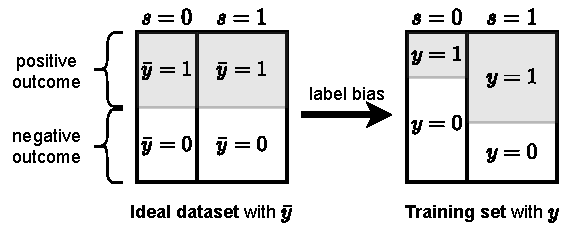
\includegraphics[width=0.9\textwidth]{figures/label_bias.pdf}
  \caption{%
    A diagram of a simple case of label bias, where both the class label \(y\) and the sensitive attribute \(s\) are binary.
    On the left, we have the ideal (possibly fictional) dataset with the target labels \(\bar{y}\),
    where the proportion of positive outcomes is the same for both demographic groups;
    and on the right, the training labels, for which the proportions are \emph{not} the same.
  }%
  \label{fig:label-bias-overview}
\end{figure}

We can interpret the contributions of this publication in two ways.
The first corresponds to the definition-centric view of dataset bias,
and the second to the ground-truth-centric view.
\begin{enumerate}
  \item
    We can say that the classifier should satisfy demographic parity in its predictions,
    and learning from a balanced training set is just one particular way to achieve this.
    In this view, the pseudo labels have no deeper meaning and are just a computational trick.
  \item
    We can see the training set as a corrupted version of a true dataset, which is balanced (\(y\perp s\)),
    and so, by learning from these pseudo labels, we are simply approximating the true dataset.
    However, we do not actually have access to the true dataset; we only know that it is balanced.
    In order to evaluate the trained model, we compute fairness metrics with respect to \ac{DP}.
\end{enumerate}
Within the paper, we sometimes jump between these two views.

While the main focus is on label bias,
the experiments are performed on real-world fairness datasets,
which also display a significant amount of sample bias (disadvantaged groups are underrepresented).
Furthermore, in addition to the result for \ac{DP}, we also show that the proposed scheme improves \acf{EOpp}.

In order to construct the target labels,
we use side information about summary statistics for a balanced training set.
This allows us to target a specific balanced set, instead of just any balanced set.
In other words, rather than just enforcing \ac{DP}, the method gives control over the target rates \(P(\hat{y}=1|s)\),
which are the only fairness-hyperparameters of the model.
The target labels \(\bar{y}\) represent an uncertain estimate of labels corresponding to a balanced dataset
(one where \(\bar{y} \perp s\); see also \figref{fig:label-bias-overview}).
The idea is then the learn a predictor for these target labels instead of the given (biased) training labels \(y\).
Via the sum rule of probabilities, it is possible to express the model likelihood in terms of the target labels,
such that maximising the likelihood corresponds to improving the prediction of the target labels.

The requirements for the model are that it outputs probabilities
and that they are well-calibrated --
which means that for those samples
that the model predicts a 10\% chance of having a positive label (\(y=1\))
about 10\% in fact have a positive label,
and analogously for all other predicted probabilities.
The probabilities are needed for calculating the expected target label,
and the calibration ensures that this expectation is sensible.
Thus, we picked a \acf{GP} model as one model for the experiments,
as they have a reputation for being well-calibrated.
However, they come with the downside that they are (at least in their standard form)
not well-suited to very high dimensional data like images.
As such, we also construct a model based on \acf{LR}.

The method is validated with experiments
on the UCI Adult Income dataset and the ProPublica/COMPAS dataset,
which have been mentioned several times in \chapref{ch:related-work},
and which are the most common tabular fairness datasets.
While both these datasets comprise only tabular data,
there is nothing in principle that stops this method from being used for other kinds of data.
The choice to use these datasets and not others
was predominantly made for easier comparison to baselines,
and shorter experiment runtime.

\section{Overcoming severe sampling bias with a representative set}\label{sec:nifr}
In the setting from the above paper \citep{kehrenberg2020tuning},
labels were untrustworthy because they had been flipped;
a phenomenon we referred to as \emph{label bias}.
However, flipping labels is not the only way that labels can become untrustworthy.
Another way is \emph{sampling bias}, which is the subject of \citet{kehrenberg2020nullsampling} and \citet{kehrenberg2020zeroshot} (\twochaprefs{ch:paper2}{ch:paper3}).

As an example, consider the scenario where someone wants to create a classifier
to distinguish between sheep and cows, that is supposed to work anywhere on earth.
However, they take a shortcut while creating the dataset
and take all their sheep images from hot and dry countries
and all their cow images from mild and rainy countries.
In this case, the dataset is lacking cow images in dry landscapes,
and is lacking sheep from green landscapes;
the dataset exhibits a strong sampling bias.
The result is that even though the labels correctly correspond to cows and sheep,
they do not point reliably to the right target anymore.
As background colour is easier to recognise with a \ac{CNN} than animal species,
the labels have effectively been turned into landscape labels.
In other words, landscape has become a \emph{spurious attribute}.
%
% As an example, consider a dataset where the task is to distinguish smiling from non-smiling faces.
% Say, we initially have a very diverse and balanced training set,
% but then, from the set of smiling faces, we remove nearly all samples where the person does not have red hair,
% and from the set of non-smiling faces, we remove nearly all samples with non-black hair.
% The result is that even though the labels are still correct, they do not point reliably to the right target anymore.
% As hair colour is easier to recognise with a \ac{CNN}, the labels have effectively been turned into hair colour labels.
% In other words, hair colour has become a \emph{spurious attribute}.
In the following, we denote the spurious attribute with \(s\),
as it takes on a role that is very similar to that of the sensitive attribute that was also denoted by \(s\).
However, there is a difference in emphasis between a \emph{sensitive} and a \emph{spurious} attribute:
the former indicates that the attribute should not be used for legal or ethical reasons,
whereas the latter can be any attribute that is associated with the class label \(y\) in an undesired way
that leads to lower quality generalisation.

The method, proposed in the previous paper (\chapref{ch:paper1}),
is not able to deal with such a dataset bias as we can easily see:
Say, \emph{smiling} corresponds to \(y=1\) and \emph{not smiling} to \(y=0\);
furthermore, let red hair correspond to \(s=1\), black hair to \(s=0\), and all other hair colours to \(s=2\).
Then, the problem with the described dataset is, that it mostly consists of samples with \(y=0\wedge s=0\)
and those with \(y=1\wedge s=1\).
If we call \(P(y=1|s=s')\) the acceptance rate,
then the problem can be described as one of very different acceptance rates in the hair colour groups given by \(s\).
This is the problem tackled in the previous paper,
and yet, if we were to equalise the acceptance rates with the method there,
the result would be very incorrect.
The issue is that we would treat the labels as incorrect, when in truth, they are correct;
the problem with the data being sampling bias.

To deal with sampling bias, a different approach is needed.
Indeed, the problem, as posed, is not solvable in the general case.
To make headway with this problem, we introduce the concept of a \emph{representative set}.
This set is not subject to the sampling bias,
but is unlabelled (with respect to $y$) and so does not by itself suffice for training.
However, this set does have labels for the spurious attribute \(s\).
This allows us to learn an \emph{invariant representation},
\ie, a representation of the input features \(x\) which is invariant to the spurious attribute.
This kind of representation is equivalent to a fair representation -- as described in \secref{sec:fair-representation} --
which is invariant to a sensitive attribute.
With the invariant representation of the training set,
a classifier can then be trained to accurately predict the class label \(y\).
The invariant representation cannot be learned from the training set
because there, due to the sampling bias, \(s\) and \(y\) are not sufficiently distinguishable.

A parallel to the previous paper is that the method makes use of side information
(in this case the representative set)
in order to overcome the bias in the training set.

The method implementing this general strategy, and presented in \citet{kehrenberg2020nullsampling} (\chapref{ch:paper2}),
is based on the idea of \emph{null-sampling},
which refers to zeroing out part of an encoding,
and then reconstructing the modified encoding as if it were a normal encoding.
In order to apply null-sampling, an encoding of the input \(x\) is learned that is split into two parts:
\(z_u\), which has no information about the spurious attribute \(s\),
and \(z_b\), which has all the remaining information needed to reconstruct \(x\) that is not contained in \(z_u\).
\(z_u\) is ensured to be not predictive of \(s\) via adversarial training.
During null-sampling, \(z_b\) is zeroed out, and after decoding it,
we obtain an invariant representation \emph{in the data domain}.
The fact that it is in the data domain makes it interpretable (or inspectable)
as defined in \chapref{ch:introduction}.

The described method works particularly well with \acp{INN},
as they ensure that no information is lost that is unrelated to \(s\).
However, the price to pay for using \acp{INN} is higher memory requirement and slower training.
Thus, we also present a variant of the method using \iac{VAE},
which does not have the guarantee about preserving information,
but also does not suffer from the increased training cost as much.
\acp{VAE} are similar to \acp{INN}
in that their encoding conforms to a specific probability distribution,
from which we can sample our null-samples.
The choice between the two presented variants is determined
by whether the user is willing to accept higher training costs
for a lower probability of losing information needed for any prediction tasks.
However, the key element is simply any kind of encoder -- producing a split-encoding --
whose output can be subjected to adversarial training,
so encoders other than \acp{VAE} or \acp{INN} will potentially work as well.

We perform experiments on the Coloured MNIST dataset (as described in \secref{sec:groundtruth-centric-view-of-bias}),
which has a one-to-one mapping between the class label (\ie, digit) and the spurious attribute (colour)
in the training set.
As colour is ``easier'' to learn, a neural network will learn to predict \(s\) instead of \(y\).
For additional experiments on the CelebA dataset (another image dataset)
and the UCI Adult Income dataset (a tabular dataset),
we deliberately apply sampling bias to the training set and then apply our method.
For the tabular dataset, an autoencoder is trained to produce a continuous representation,
which is then fed into the \ac{INN} or \ac{VAE} model.
Thus, we demonstrate that the method is \emph{general}
in the sense that it is applicable to both image-based and tabular datasets
and furthermore should be applicable to other modalities as well.
For the main experiments, we focus on image datasets,
because they are easiest to visualise in a document.

\section{Overcoming sampling bias with an unlabelled deployment set}\label{sec:zsf}
A shortcoming of the approach from the previous publication \citep{kehrenberg2020nullsampling}
is its reliance on a representative set which has labels for the spurious attribute \(s\).
As discussed, it is necessary to make use of \emph{some} kind of side information,
but perhaps we can relax some requirements.
In particular, while it is already easier to collect data without \(y\) labels (but with \(s\) labels),
it is even easier to collect data without \emph{any} label.
Thus, requiring only an unlabelled context set would improve the applicability of the method.
\citet{kehrenberg2020zeroshot} (\chapref{ch:paper3}) presents an approach based on that idea.

The setting is very similar to the previous publication \citep{kehrenberg2020nullsampling}:
the training set suffers from severe sampling bias, but we have access to a (mostly) unbiased \emph{deployment set}
(similar to but not quite identical to the previously discussed \emph{representative set}).
The idea is that the deployment set corresponds to the setting in which the model is meant to be deployed.
The change from the previous setting is that this additional set may be completely unlabelled,
but in exchange, we have some stronger requirements for the training set:
The holes left by the sampling bias may not be so numerous
as to make \(s\) and \(y\) completely indistinguishable.
For example, in the previous work, the example of Coloured MNIST had a training set
where there was a strict one-to-one mapping of colour and digit;
but this kind of blending of \(s\) and \(y\) into one is not the focus of this paper.
Instead, the focus is on a setting where the training set lacks certain combinations of \(s\) and \(y\),
which results in poor predictions for these combinations on the test set (or deployment setting)
where those combinations \emph{do} occur.
We refer to these missing combinations as \emph{subgroup bias} or \emph{missing subgroups},
depending on whether a given \(s\) value appears in the training set at all.
The label \(s\) plays here a similar role to the spurious attribute in the previous publication,
but as there is a change in emphasis, we refer to \(s\) as \emph{subgroup label}%
\footnote{This terminology is inspired by the \emph{subclass} concept in \citet{SohDunAngGuetal20}.}
instead.
The difference between a spurious attribute and a subgroup label is that
the former is mostly characterised via its confusion with the prediction target,
whereas the latter refers to natural groups in the data
which have differing levels of annotation quality which affects the classification performance on these subgroups.
However, in both cases, the goal is to make the model output invariant to the \(s\) label,
\ie the classification performance should be independent of the subgroup.

As in the previous paper, the first step is to train a neural network to produce an invariant representation.
The second step is then to train a classifier on said representation.
The invariant representation is trained by performing \emph{distribution matching} between the training set and the deployment set.
% Finally, the training set is transformed into the invariant representation,
% to serve as training set for the classifier.

The distribution matching is realised with adversarial networks which compare batches of samples,
in order to try to distinguish data drawn from the training set and the deployment set.
This process requires balanced batches as an inductive bias,
because the network will only learn the intended difference between training and deployment set,
if the drawn batches exhibit this difference.
For example, if batches drawn from Coloured MNIST differ not in colour but in digit class,
then distribution matching will learn to change digit shapes.
Balancing batches from the training set is easily possible with the available labels,
but those are not available for the deployment set,
so we use clustering techniques to identify the different groups in the deployment set,
and then draw samples for the batches at an equal rate from all clusters.
It is important to note here that imperfections in the clustering are not a problem
as long as the batches show on average the intended difference between training and deployment set.

The absolutely essential elements for this method are the encoder (also referred to as `de-biaser')
that encodes both, samples from the training set and samples from the deployment set,
to a splittable representation;
the adversary that tries to identify, from one part of the split representation,
which dataset the given samples originated from;
and some kind of reconstruction loss
to ensure the splittable representation represents the input data well.
The following elements are in theory optional,
but are needed for the method to work with real-world data:
clustering and sampling to ensure that the training batches are balanced in specific ways;
subdivision of the batches into bags; and the aggregation of the adversarial loss over the bags.
Roughly speaking, these elements strengthen the supervision signal for the invariance learning.

Experiments are performed on the same datasets as in the previous papers:
Coloured MNIST, UCI Adult Income and CelebA.
Again, these datasets were chosen, because image data is easy to visualise,
and because demonstrating the method on tabular data provides evidence for the generality.

% \section{Claims and contributions}%
\section{List of publications and author contributions}%
\label{sec:claims-contributions}
This thesis is based on 3 publications (one of which is a work in progress),
corresponding to \rangechapref{ch:paper1}{ch:paper3}.
% The first one is concerned with \emph{label bias} and the other two with \emph{sampling bias}.
The following is a detailed listing of all the individual author contributions.

\subsection{Publication 1}
\begin{refsection}[allreferences]
    \nocite{kehrenberg2020tuning}
    \printbibliography[heading=none]
\end{refsection}
\noindent A shorter version was published as a workshop paper:
\begin{refsection}[allreferences]
    \nocite{kehrenberg2018interpretable}
    \printbibliography[heading=none]
\end{refsection}
\noindent\textsc{Contributions:}
\begin{itemize}
  \item I conceived the idea of using Target Labels to target a balanced set.
    I developed the proof from a starting point that my supervisor pointed me to.
    I wrote all of the code dealing with the modified loss function and nearly all of the remaining code as well.
    I ran most of the experiments and wrote all of the methods section and most of the remaining text as well.
  \item Z. Chen was a discussion partner and helped run the experiments, and wrote some parts of the code.
  \item N. Quadrianto suggested the initial direction of the work, was a discussion partner,
    and helped write the introduction and related work.
\end{itemize}

\subsection{Publication 2}
\begin{refsection}[allreferences]
    \nocite{kehrenberg2020nullsampling}
    \printbibliography[heading=none]
\end{refsection}%
\noindent\textsc{Contributions:}
\begin{itemize}
  \item I conceived the idea of using an \acf{INN} and a representative set to learn an invariant representation.
    I wrote a large part of the code, and ran about half the experiments. I wrote a significant part of the text.
  \item M. Bartlett developed a large part of the tricks needed for training the \ac{INN} successfully.
    He wrote a significant part of the code, and of the text.
  \item O. Thomas helped with writing the code and with running the experiments.
  \item N. Quadrianto gave feedback on the progress and suggested directions to explore.
\end{itemize}

\subsection{Publication 3 (work in progress)}
\begin{refsection}[allreferences]
    \nocite{kehrenberg2020zeroshot}
    \printbibliography[heading=none]
\end{refsection}%
\noindent\textsc{Contributions:}
\begin{itemize}
  \item I developed the idea of distribution matching as an extension of the previous paper.
    In addition, I tried to achieve similar goals by applying clustering to an unlabelled auxiliary set,
    with supervision from the labelled training set.
    I wrote all of the initial implementation of the method, and a large part of the later refined implementation.
    I ran the majority of the experiments.
  \item V. Sharmanska developed the original link to a fairness problem
    and wrote parts of the introduction and related work and contributed to other sections.
  \item M. Bartlett introduced the idea of batches-of-bags.
    He also improved the \ac{NN} architectures of the encoder and the discriminator,
    ran experiments, wrote the sections on architecture and contributed to other parts of the paper.
  \item N. Quadrianto suggested how to combine the two research directions that I had into a coherent whole.
    He also gave general feedback and suggested directions to explore.
\end{itemize}


\cleardoublepage
\ctparttext{
  This part comprises two peer-reviewed publications and one work in progress.
  They are reproduced here with minimal changes.
}
\part{Publications}\label{pt:main}

% \begin{refsection}[nifr]
%   % -------------------------------------------------------------------------------
\chapter{Null-sampling for Interpretable and Fair Representations}\label{ch:nifr}
% -------------------------------------------------------------------------------
\textsc{Authors}:\\
%
Thomas Kehrenberg$^1$,
%
Myles Bartlett$^1$,
%
Oliver Thomas$^1$ \&
%
Novi Quadrianto$^{1,2,3}$ \\
%
\textsc{Affiliations}:\\
%
$^1$Predictive Analytics Lab (PAL), University of Sussex, Brighton, UK\\
%
$^2$BCAM Severo Ochoa Strategic Lab on Trustworthy Machine Learning \\
%
$^3$Monash University, Indonesia \\
%
\textsc{Conference}:\;\;\textit{European Conference on Computer Vision} (ECCV), 2020 \\
%
\textsc{DOI}:\;\;\texttt{10.1007/978-3-030-58574-7\_34} \\
%
\textsc{Note}:\;\;The appendices have been included as \S\ref{sec:nifr-appendix}.
%

% -------------------------------------------------------------------------------
\section{Abstract}
\noindent
We propose to learn invariant representations, in the data domain, to achieve interpretability in
algorithmic fairness. Invariance implies a selectivity for high level, relevant correlations
w.r.t.\ class label annotations, and a robustness to irrelevant correlations with protected
characteristics such as race or gender. We introduce a non-trivial setup in which the training set
exhibits a strong bias such that class label annotations are irrelevant and spurious correlations
cannot be distinguished. To address this problem, we introduce an adversarially trained model with
a \emph{null-sampling} procedure to produce invariant representations in the data domain. To enable
disentanglement, a partially-labelled \emph{representative} set is used. By placing the
representations into the data domain, the changes made by the model are easily examinable by human
auditors. We show the effectiveness of our method on both image and tabular datasets: Coloured
MNIST, CelebA, and the Adult dataset.

\section{Introduction}
% We need to stare start with something with more punch
%r rather than just a f matter-of-fact statement Fair representations are a means of removing
%potentially sensitive information from training data in order to avoid wrongly relying on the
%sensitive information for classification.
Without due consideration for the data collection process, machine learning algorithms can
exacerbate biases, or even introduce new ones if proper control is not exerted over their learning
\citep{holstein2019improving}. 
%
While most of these issues can be solved by controlling and curating data collection in a
fairness-conscious fashion, doing so is not always an option, such as when working with historical
data. 
%
Efforts to address this problem algorithmically have been centred on developing statistical
definitions of fairness and learning models that satisfy these definitions. 
%
One popular definition of fairness used to guide the training of fair classifiers, for example, is
\emph{demographic parity}, stating that positive outcome rates should be equalised (or
\emph{invariant}) across protected groups.

In the typical fair-classification setup, we have an input $x \in \gX$, a sensitive attribute $s
\in \gS$, that represents some inadmissible (for prediction) information like gender and a class
label $y \in \gY$ which is the prediction target. 
%
The idea of fair \emph{representation} learning
\citep{zemel2013learning,edwards2016censoring,madras2018learning} is then to transform the input
$x$ to a representation $z \in \gZ_{\neg s}$ which is invariant to $s$, so that in training a
downstream predictor on that representation one cannot introduce a forbidden dependence on $s$.
% $\bm{z}$ can then be used to learn a predictor In fair representation learning
% \cite{zemel2013learning}\cite{edwards2016censoring}\cite{madras2018learning}, the goal is then to
% find a representation $\bm{z}$ that is invariant to $s$.
A good fair representation is one that preserves most of the information from $x$ while
satisfying the aforementioned constraints.
% While fair \emph{representations} are by no means the only method of achieving this goal,
% approaches that explicitly depend on the target label \cite{kamiran2012data} are restrictive in
% that they do not readily admit transfer to unseen tasks, and are bound by the requirement of
% having $s$ and $y$ labels be present together.

As unlabelled data is much more freely available than labelled data, it is of interest to learn the
representation in an unsupervised manner. 
%
This will allow us to draw on a much more diverse pool of data to learn from.
% ; this is particularly pertinent for fair representation learning as unlabelled data affords us a
% much more diverse pool of data to learn from.
%To this end, \cite{locatello2019fairness} recently made the connection from disentangled
%representations to fair representations: a model for disentanglement trained without knowledge of
%the sensitive attribute $s$ nevertheless appears to improve fairness measures with respect to $s$.
%However, as pointed out by \cite{locatello2019challenging}, some supervision or inductive bias is
%needed in order to recognise a well-disentangled representation.
While annotations for $y$ are often hard to come by (and often noisy;
see~\cite{kehrenberg2020tuning}), annotations for the sensitive attribute $s$ are usually less so,
as $s$ can often be obtained from demographic information provided by census data. 
%
We thus consider the setting where the representation is learned from data that is only labelled
with $s$ and not $y$. 
%
This is in contrast to most other representation learning methods.
% We thus consider the setting where data labelled with $s$ (partially labelled data) is available
% for learning the fair representation. Furthermore, we assume the existence of a set with $s$
% labels whose distribution matches the deployment setting
We call the set used to learn the representation the \emph{representative} set, because its
distribution is meant to match the distribution of the deployment setting (and is thus
representative).
% We call this set the \emph{representative} set and its distribution is meant to match the
% distribution of the deployment setting.

Once we have learnt the mapping from $x$ to $z$, we can transform the \emph{training} set
which, in contrast to the representative set, has the $y$ labels (and $s$ labels). 
%
In order to make our method more widely applicable, we consider an \emph{aggravated fairness
problem}
% we allow the case
in which the training set contains a strong spurious correlation between $s$ and $y$, which makes
it impossible to learn from it a representation which is invariant to $s$ but not invariant to $y$,
variance to $y$ being important as this is the variable we care about predicting accurately. 
%
The training set thus does \emph{not} match the deployment setting, thereby rendering the
representative set essential for learning the right invariance.
% We also tackle the related problem of learning from biased data, specifically cases in which the
% training set (with $y$ labels) contains a strong spurious correlation between $s$ and $y$, and
% thus does not match the deployment setting.
Throughout the remainder of the paper, we will use the terms \emph{spurious} and \emph{sensitive}
interchangeably, depending on the context, to refer to an attribute of the data we seek invariance
to.
% This is essentially a form of strong sampling bias and is not an unrealistic complication, having
% been shown to plague real-world datasets \cite{kallus2018residual}.
%Classifiers trained on ImageNet for example, have been shown to be biased towards texture
%\cite{Geir18}. \cite{zhang2018visual} similarly examine the problem of learning from biased data,
%showing that pre-trained models can exploit biases in the data by learning patterns semantically
%unrelated to the target, an issue that can be difficult to identify when the bias pervades both
%the training and test sets.
We can draw a connection between learning in the presence of spurious correlations and what
\citet{kallus2018residual} call \emph{residual unfairness}. 
%
Consider the Stop, Question and Frisk (SQF) dataset for example: the data was collected in New York
City, but the demographics of the recorded cases do not represent the true demographics of NYC
well. 
%
The demographic attributes of the recorded individuals might correlate so strongly with the
prediction target that the two are nearly indistinguishable. 
%
This is the scenario that we are investigating: $s$ and $y$ are so closely correlated in the
labelled dataset that they cannot be distinguished, but the learning of
$s$ is favoured due to its lower complexity.
%
The deployment setting (i.e.\ the test set) does not possess this strong correlation and thus a
na\"ive approach will lead to very unfair predictions. 
%
In this case, a disentangled representation is insufficient; the representation needs to be
explicitly invariant solely with respect to $s$. 
%
In our approach, we make use of the (partially labelled) representative set to learn this invariant
representation.

While there is a substantial body of literature devoted to the problems of fair
representation-learning, exactly how the invariance in question is achieved is often overlooked.
%
When critical decisions, such as who should receive bail or be released from jail, are being
deferred to an automated decision making system, it is critical that people be able to trust the
logic of the model underlying it, whether it be via semantic or visual explanations. 
%
We build on the work of \citet{QuaShaTho19} and learn a decomposition ($f^{-1}: (\gZ_s \times
\gZ_{\neg s}) \to \gX$) of the \emph{data domain} ($X$) into independent subspaces
\emph{invariant} to  $s$ ($\gZ_{\neg s}$) and \emph{variant} to $s$ ($\gZ_{s}$), which lends an
interpretability that is absent from most representation-learning methods. 
%
While model interpretability has no strict definition \citep{zhang2018visual}, we follow the
intuition of \citet{adel2018discovering} -- \emph{a simple relationship to something we can
understand}, a definition which representations in the data domain naturally fulfil.

Whether as a result of the aforementioned sampling bias or simply because the features necessarily
co-occur, it is not rare for features to correlate with one another in real-world datasets.
%
Lipstick and gender for example, are two attributes that we expect to be highly correlated and to
enforce invariance to gender can implicitly enforce invariance to make-up. 
%
This is arguably the desired behaviour. 
%
However, unforeseen biases in the data may engender cases which are less justifiable. 
%
By baking interpretability into our model (by having representations in the data domain), though we
still have no better control over what is learned, we can at least diagnose such pathologies.

To render our representations interpretable, we rely on a simple transformation we call
\emph{null-sampling} to map invariant representations in the data domain. 
%
Previous approaches to fair representation learning
(\cite{beutel2017data,edwards2016censoring,madras2018learning,louizos2016variational}, inter alia)
predominantly rely upon autoencoder models to jointly minimise reconstruction loss and invariance. 
%
We discuss first how this can be done with such a model that we refer to as cVAE (conditional VAE),
before arguing that the bijectivity of invertible neural networks (INNs)~\citep{Dinh2014} makes
them better suited to this task. 
%
We refer to the variant of our method based on these as cFlow (conditional Flow). 
%
INNs have several properties that make them appealing for unsupervised representation learning. 
%
The focus of our approach is on creating invariant representations that preserve the non-sensitive
information maximally, with only knowledge of $s$ and not of the target $y$, while at the same time
having the ability to easily probe what has been learnt.

% The problem of fair representations can also be viewed through a similar lens. A good toy model
% for this setup is the Coloured MNIST (cMNIST) dataset. In this example, the colour is a spurious
% variable which is very closely correlated with the prediction target in the training set but not
% in the deployment setting. An interpretable invariant representation in this case is the images
% uniform in colour. More details regarding the setup and synthesis of the dataset can be found in
% section~\ref{ssec:cmnist}.

% As a more real-world dataset, we consider the CelebA dataset. We treat the CelebA dataset as it
% is, as the deployment setting and construct deliberately biased subsets of CelebA to serve as the
% training set. In our experiments we use gender as the sensitive attribute. Sample images can be
% seen in \thomas{Fig.??}. Attributes that are correlated with gender in the \emph{deployment
% setting} (like the use of lipstick) will also be removed by our method. We do not consider this a
% defect of our method and instead argue that this is the correct behaviour: As long as the
% deployment setting is sufficiently diverse, the model may make use of correlations found in
% there.
%wearing lipstick is a valid indicator of gender. \thomas{maybe don't include the previous
%sentence}

Our contributions are thus two-fold: 
%
1) We propose a simple approach to generating representations that are invariant to a feature $s$,
while having the benefit of interpretability that comes with being in the data domain. 
%
We call our method \emph{NIFR} (\emph{N}ull-sampling for \emph{I}nterpretable and \emph{F}air
\emph{R}epresentations).
%
2) We explore a setting where the labelled training set suffers from varying levels of sampling
bias, demonstrating an approach based on transferring information from a more diverse
representative set, with guarantees of the non-spurious information being preserved.

\section{Background}\label{sec:background}
% \noindent We frame our approach in the context of relevant literature on the interrelated
% problems of fair representation learning and learning representations free of spurious
% correlations. The background is far too long - we also need to touch on the interpretability
% literature

\subsection{Learning fair representations.}
%As we have alluded to, the goal of producing invariant representations is similar to that of
%producing \emph{fair} representations. In fairness problems, there is usually a \emph{sensitive
%attribute}, $s$ (for example, gender or race), that should not be used to make decisions.
Given a sensitive attribute $s$ (for example, gender or race) and inputs $x$, a fair
representation $z$ of $x$ is then one for which $z \perp s$ holds, while ideally
also being predictive of the class label $y$. 
%
\citet{zemel2013learning} was the first to propose the learning of fair representations which allow
for transfer to new classification tasks. More recent methods are often based on
\acfp{VAE}~\citep{kingma2013auto,louizos2016variational,edwards2016censoring,beutel2017data}. The
achieved fairness of the representation can be measured with various fairness metrics. These
measure, however, usually how fair the predictions of a classifier are and not how fair a
representation is.

The appropriate measure of fairness for a given task is domain-specific \citep{liu2018delayed} and
there is often not a universally accepted measure. However, \emph{Demographic Parity} is the most
widely used~\citep{louizos2016variational,edwards2016censoring,beutel2017data}. Demographic Parity
demands $\hat{y} \perp s$ where $\hat{y}$ refers to the predictions of the classifier. In the
context of fair representations, we measure the Demographic Parity of a downstream classifier,
$f(\cdot )$, which is trained on the representation $z$, i.e.\  $\Gamma: \gZ \to \gY$.

A core principle of all fairness methods is the \emph{accuracy-fairness trade-off}. As previously
stated, the fair representation should be invariant to $s$ ($\to$ fairness) but still be predictive
of $y$ ($\to$ accuracy). These desiderata cannot, in general, be simultaneously satisfied if $s$
and $y$ are correlated.

The majority of existing methods for fair representations also make use of $y$ labels during
training, in order to ensure that $z$ remains predictive of $y$. This aspect can, in theory,
be removed from the methods, but then there is no guarantee that information about $y$ is preserved
\citep{louizos2016variational}. 
% Existing methods designed to create fair representations can, in theory, be extended to the
% regime in which only the $s$, and not the $y$, labels are available. However, it is not without
% its drawbacks as, in removing $s$, there is no guarantee that information about $y$ is preserved
% \cite{louizos2016variational}. For this reason, $y$ is typically supplied during training and the
% representation encouraged to be predictive of it.

\subsection{Learning fair, transferrable representations}
% Outside of computer vision, \cite{madras2018learning} have also worked on removing a problematic
% spurious correlation.
In addition to producing fair representations, \citet{madras2018learning} want to ensure the
representations are transferable. Here, an adversary is used to remove sensitive information from
a representation $z$. Auxiliary prediction and reconstruction networks, to predict class label $y$
% to ensure it remains predictive of $y$
and reconstruct the input $x$ respectively, are trained on top of $z$, with $s$ being ancillary
input to the reconstruction.
% alongside a reconstruction loss computed with respect to the output of a decoder that takes $z$
% and the sensitive label $s$ as input is added. This is so that $x$ can still be reconstructed
% from $z$, despite the removal of $s$.
%The decoder is utilised only for the purpose of maximum likelihood learning of the data
%distribution. By conditioning the decoder on the sensitive attribute, information about it can be
%``off-loaded'' from the encoder such that information about $s$ need not be contained in the fair
%representation while still permitting the use of a reconstruction loss needed to capture
%non-sensitive information. The decoder plays a role only in the loss function. In contrast, we
%make explicit use of the decoder not only for characterising the behaviour of the model and also
%for evaluation.

Also related is \citet{creager2019flexibly} who employ a FactorVAE \citep{kim2018disentangling}
regularised for fairness. 
%
The idea is to learn a representation that is both disentangled and invariant to multiple sensitive
attributes. 
%
This factorisation makes the latent space easily manipulable such that the different subspaces can
be freely removed and composed at test time. Zeroing out the dimensions or replacing them with
independent noise imparts invariance to the corresponding sensitive attribute. 
%
This method closely resembles ours when we use an invertible encoder. 
%
However, the emphasis of our approach is on interpretability, information-preservation, and coping
with sampling bias - especially extreme cases where \( |\gS^{tr} \times \gY^{tr}| < | \gS^{te}
\times \gY^{te} | \).
% Namely, the invertibility of the network means we can optimise for invariance singularly without
% the burden of a reconstruction loss. While we do not explicitly consider the case of
% multi-attribute fairness, our method can be easily adapted for this use-case.

Attempts were made by~\citet{QuaShaTho19} prior to this work to learn fair representations in the
data domain in order to make it interpretable and transferable. In their work, the input is assumed
to be additively decomposable in the feature space into a \emph{fair} and \emph{unfair} component,
which together can be used by the decoder to recover the original input. This allows us to examine
representations in a human-interpretable space and confirm that the model is not learning a
relationship reliant on a sensitive attribute. Though a first step in this direction, we believe
such a linear decomposition is not sufficiently expressive to fully capture the relationship
between the sensitive and non-sensitive attributes. Our approach allows for the modelling of more
complex relationships.

\subsection{Learning in the presence of spurious correlations}
% As  previously  discussed,  the  goal  of  producing  fair representations is similar to the goal
% of producing representations invariant to spurious correlations found in the training data.
Strong spurious correlations make the task of learning a robust classifier challenging: the
classifier may learn to exploit correlations unrelated to the true causal relationship between the
features and label, and thereby fail to generalise to novel settings. This problem was recently
tackled by \citet{kim2019learning} who apply a penalty based on the mutual information between the
feature embedding and the spurious variable. While the method is effective under mild biasing, we
show experimentally that it is not robust to the range of settings we consider.

\citet{JacBehZemBet19} explore the vulnerability of traditional neural networks to spurious
variables -- e.g., textures, in the case of ImageNet \citep{Geir18} -- and propose a INN-based
solution akin to ours. The INN's encoding is split such that one partition, $z_b$ is encouraged to
be predictive of the spurious variable while the other serves as the logits for classification of
the semantic label. Information related to the nuisance variable is ``pulled out'' of the logits as
a result of maximising $\log p(s|z_n)$. This specific approach, however, is incompatible with the
settings we consider, due to its requirement that both $s$ and $y$ be available at training time.

Viewing the problem from a causal perspective, \citet{arjovsky2019invariant} develop a variant of
empirical risk minimisation called invariant risk minimisation (IRM). The goal of IRM is to train a
predictor that generalises across a large set of unseen environments; because variables with
spurious correlations do not represent a stable causal mechanism, the predictor learns to be
invariant to them. IRM assumes that the training data is not \emph{iid} but is partitioned into
distinct environments, $e \in E$. The optimal predictor is then defined as the minimiser of the sum
of the empirical risk $R_e$ over this set. In contrast, we assume possession of only a single
source of \emph{labelled}, albeit spuriously-correlated, data, but that we have a second source of
data that is free of spurious correlations, with the benefit being that it only needs to be
labelled \emph{with respect to $s$}.

% The model thereby enforces their independence. This is achieved with an adversarial approach,
% borrowing the gradient reversal technique from \cite{ganin2016domain}.
%The authors construct the coloured MNIST dataset in two steps. First, ten distinct colours are
%assigned to each digit uniquely; these colours parameterise the means of ten corresponding
%Gaussian distributions from which colour samples are drawn. The standard deviation ($\sigma$) of
%the Gaussian distribution controls the dispersion of the sampled colours around these means. To
%demonstrate the effectiveness of their model, \cite{kim2019learning} construct a coloured version
%of the MNIST dataset as follows. During training, colours are sampled from a Gaussian distribution
%(with standard deviation $\sigma$) where each digit is associated with a single fixed mean colour.
%the colours are sampled abiding by this one-to-one colour mapping; At test time however, a colour
%mean is chosen at random from the 10 mean colours used during training. The actual colour is
%sampled with the same $\sigma$ as in the training set. there is no such designation and colours
%are sampled randomly and unrestrictedly from the complete palette. As such, a classifier that
%lazily minimises its loss by treating the pixel values as a lookup table falls flat at inference
%owing to a shift in the distribution of the spurious variables away from that of the target's. We
%follow this approach to evaluate performance of our NoSiNN framework in a synthetic setting (see
%Fig. \ref{fig:cmnist} for qualitative results).

% For the training strategy of the \cite{kim2019learning} model, a neural network is trained to
% predict the digit class, $y$, while an adversarial network takes one of the intermediate layers
% as input to predict the spurious value, colour. The first network seeks to prevent the adversary
% from making correct predictions, which means discarding or obfuscating information about colour.
% For this approach to work, the adversary needs to be able to distinguish between the digit class
% and the colour. To do this, the adversary is allowed access to the sampled RGB values of the
% colour that it is trying to remove, and not just the mean. As the sampled colour varies according
% to the standard deviation of the Gaussian distribution, the actual colour and the digit class
% vary in correlation. As the colour becomes less descriptive of the digit class, the network
% learns to disentangle the two. This works better, the larger $\sigma$; a major limitation of the
% approach its failure to deal with extremely low $\sigma$ values.


% \begin{itemize} \item Pix2pix and CycleGANs combined standard cGAN discriminators with L1
% reconstruction loss in data domain, the latter doing so in the form of cycle consistency,
% allowing for translation between unpaired samples. Bidirectional GANs extend the GAN
% discriminator to act on the distributions in data and latent space jointly. \item StarGAN
% \cite{choi2018stargan} provides a unified framework for performing image-to-image translation
% across multiple domains. \item Instead of enforcing bijectivity through cycle loses, invertible
% neural networks are bidirectional by design \item Glow achieves impressive attribute
% manipulations \item Rather than trying to translate inputs across domains we seek to do so to a
% subspace which does not abide in either domain. 
    
% \end{itemize}

% \paragraph{Unsupervised approaches.} There is a large literature on the unsupervised
% disentangling of representations; we highlight one of the more recent findings connected with our
% approach. \cite{locatello2019challenging} evidence  that the unsupervised learning of
% disentangled representations requires inductive biases on the part of both the data set and the
% models. Thus, such methods can usually only be used for a single task or kind of data.

\section{Interpretable Invariances by Null-Sampling}\label{ssec:general}
% \begin{figure}
%     \centering
%     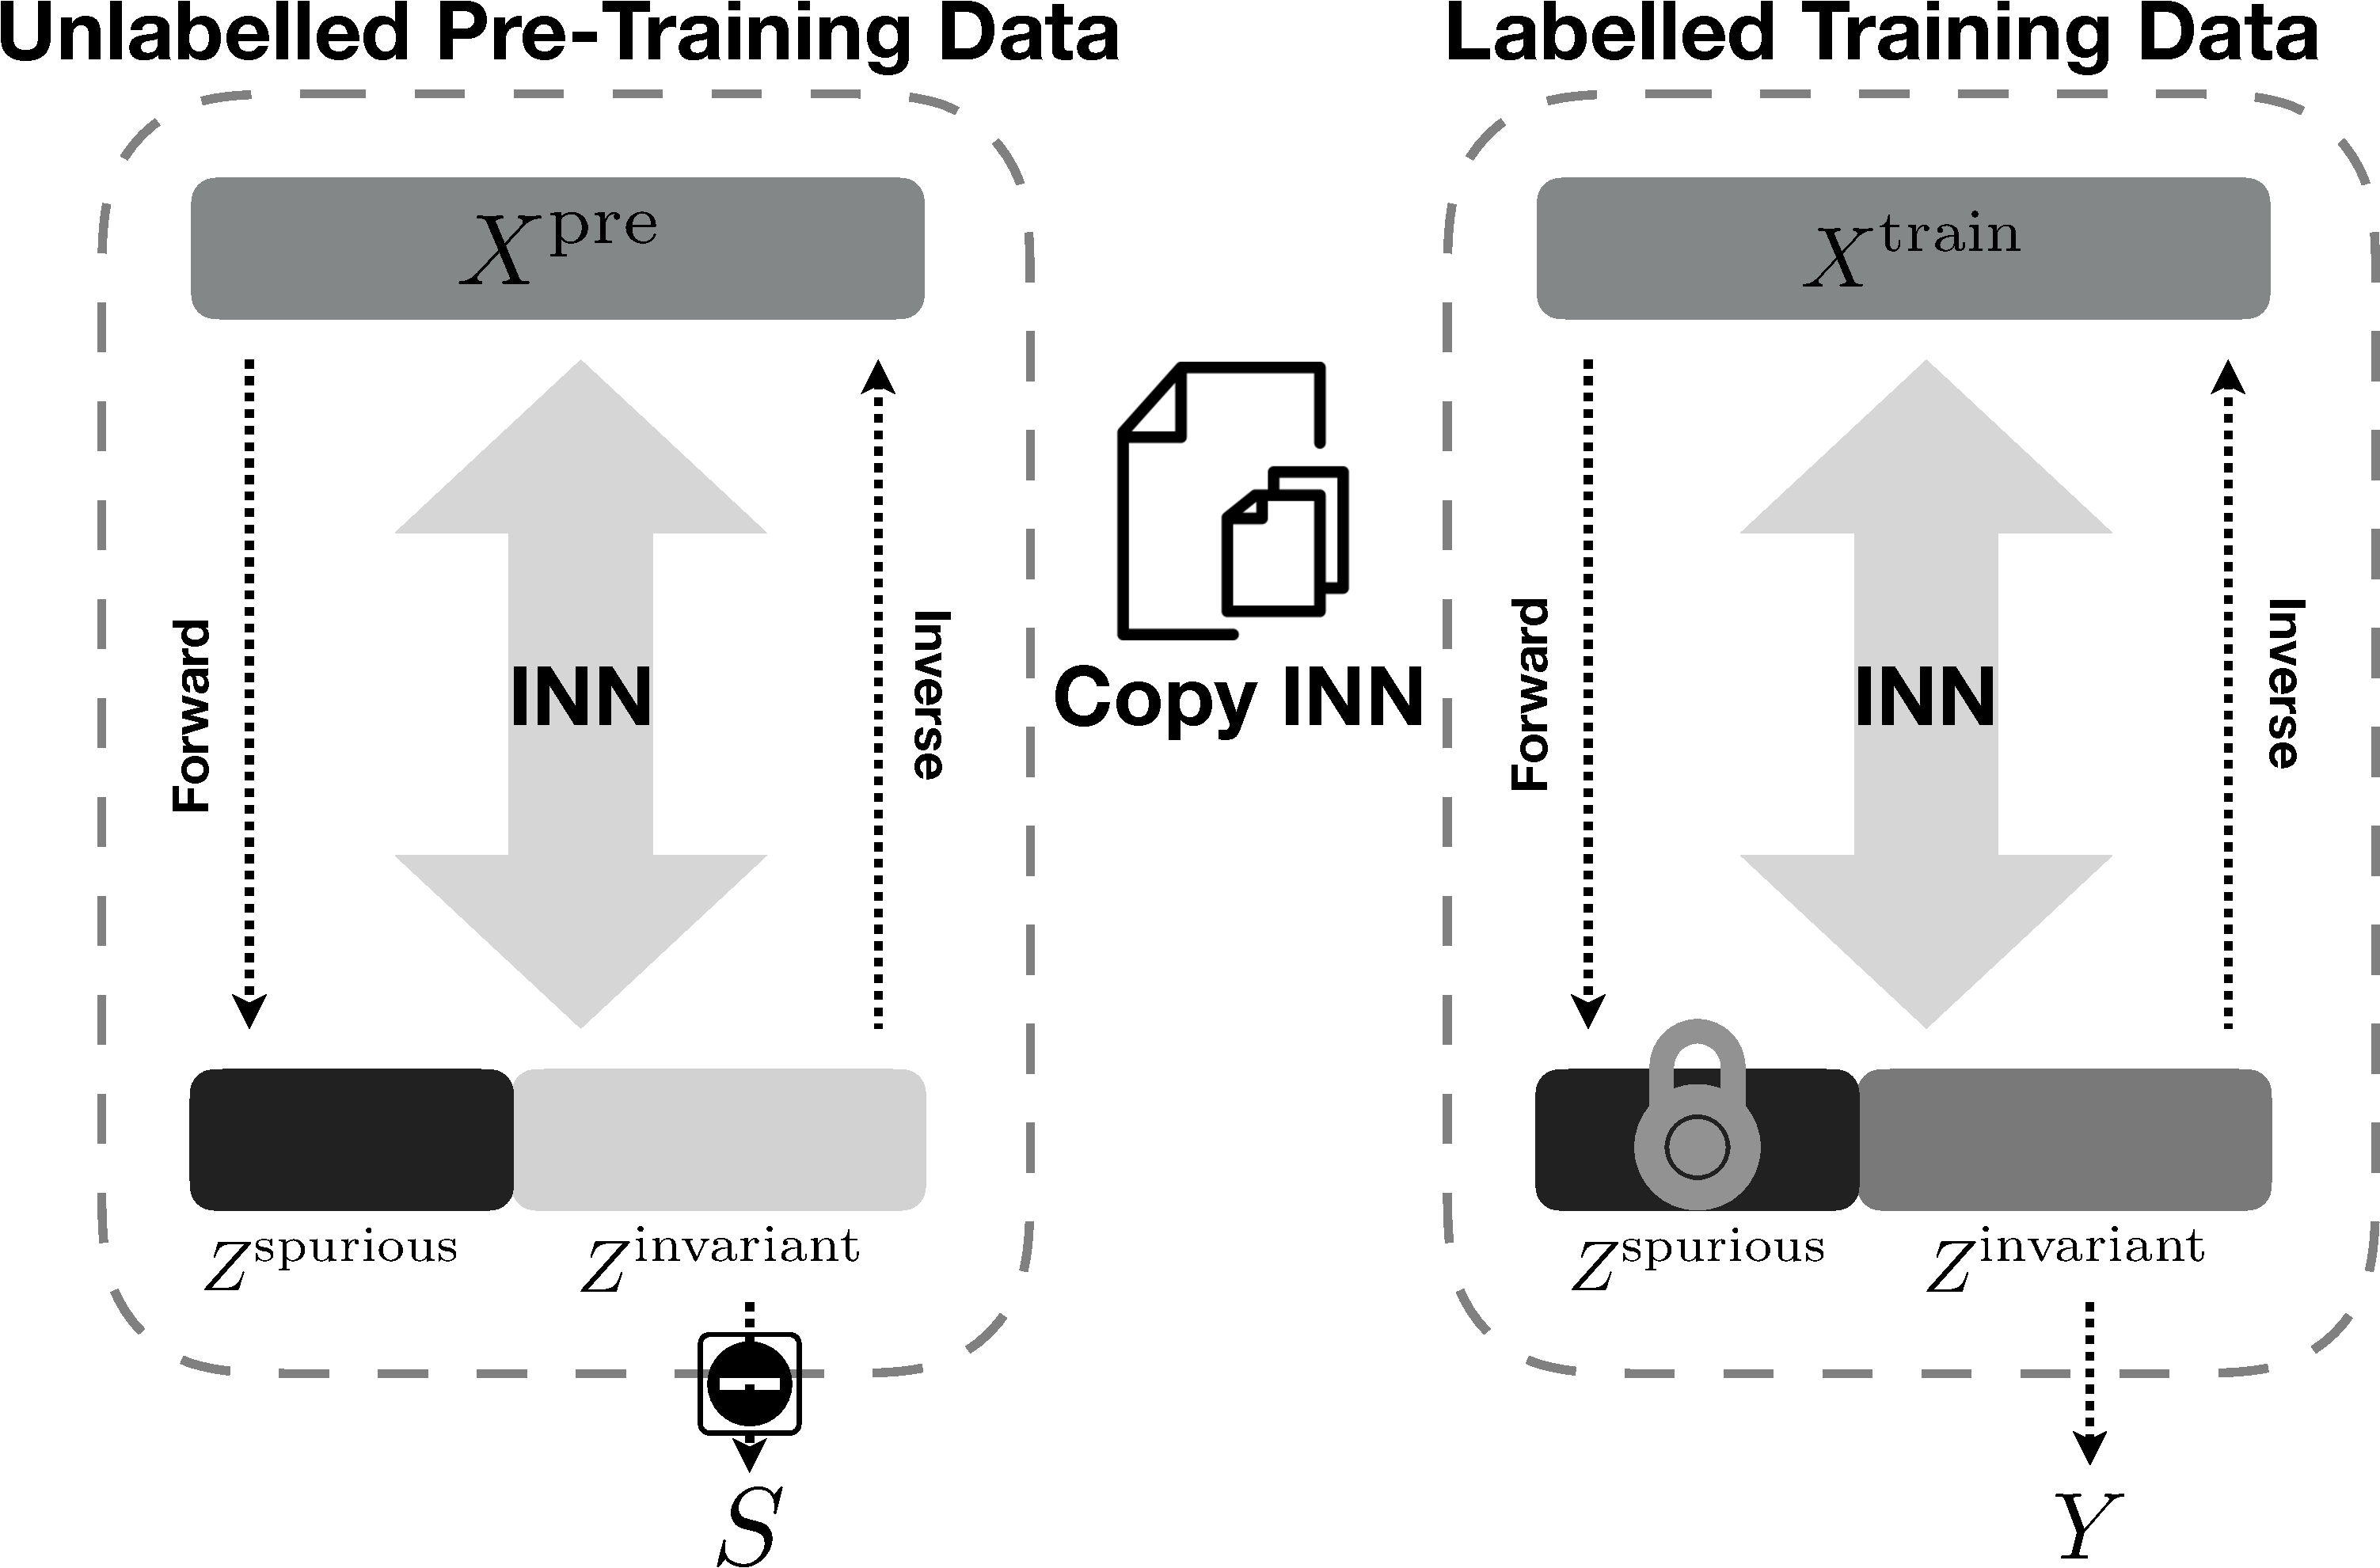
\includegraphics[width=0.4\textwidth]{nifr/Figures/diagram.pdf}
%     \caption{Training procedure using the cFlow model for illustrative purposes.}%
%     \label{fig:training_diagram}
% \end{figure}
\begin{figure*}[tb]
    \centering
    \hfill
    \subfloat[cFlow model.]{%
        \scalebox{0.4}{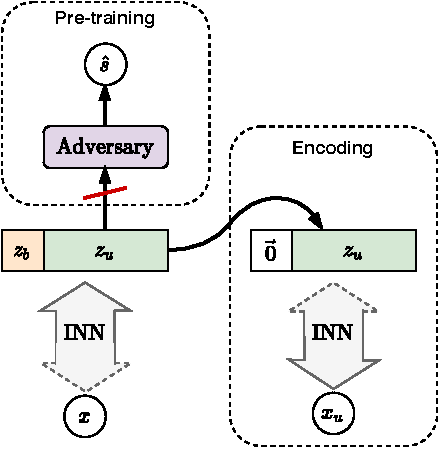
\includegraphics[width=\textwidth]{nifr/Figures/inn_diagram_u.pdf}}%
        \label{fig:inn_diagram}
    }
    \hfill
    \subfloat[cVAE model.]{%
        \scalebox{0.5}{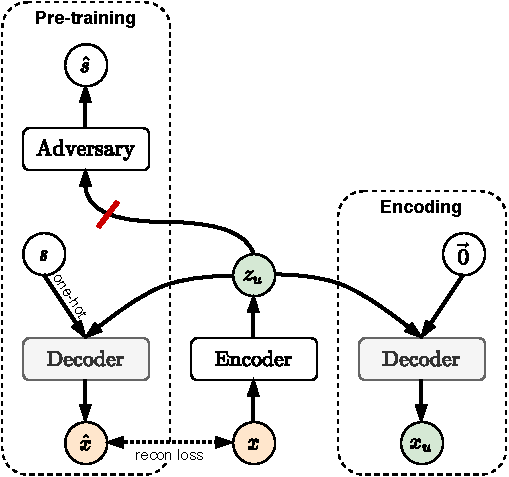
\includegraphics[width=\textwidth]{nifr/Figures/cvae_diagram_u.pdf}}%
        \label{fig:cvae_diagram}
    }
    \hfill
    \caption{
        Training procedure for our models. $x$: input, $s$: sensitive attribute, $z_u$: de-biased
        representation, $x_u$: de-biased version of the input in the data domain. The red bar
        indicates a gradient reversal layer, and $\vzero$ the null-sampling operation.
    }%
    \label{fig:model-diagrams}
\end{figure*}

\subsection{Problem Statement}
%
\noindent
%
We assume we are given inputs $x \in \gX$ and corresponding labels $y \in \gY$.
%
Furthermore, there is some spurious variable $s \in \gS$ associated with each input $x$ which
we do \emph{not} want to predict. 
%
Let $X$, $S$ and $Y$ be the random variables that take on the observed values $x$, $s$ and $y$,
respectively. 
%
The fact that both $Y$ and $S$ are predictive of $X$ implies that $\gI(X;Y), \gI(X;S) > 0$, where
$\gI(\cdot ;\cdot)$ denotes \ac{MI} between two random variables.
%
Note, however, that the conditional entropy is non-zero: \( H(S|X) > 0 \), i.e.\ $S$ is \emph{not}
completely determined by $X$.

%The difficulty emerges in the construction of the fully-supervised training dataset in which
%correspondence between $S$ and $Y$ is exaggerated compared to the test set.
The difficulty of this setup resides in the fact there is a close correspondence between $S$ and
$Y$ in the training set such that for a classifier trained via maximum-likelihood estimation, the
mappings \( \gX \to \gS \) and \(\gX \to \gY \) are functionally equivalent, which implies, through
transitivity, that \(\gX \to \gS \to \gY \) also is; in many cases, such as those we consider in
this paper, the first part of the chain, \( \gX \to \gY \), is substantially easier to learn than
the direct, and, importantly, \emph{causal}, path.
%
This is problematic when we assume that the same correlation does \emph{not} hold in the test set,
meaning the model cannot rely on shortcuts provided by $S$ if it is to generalise from the training
set.

We call this scenario where we only have access to the labels of a biasedly-sampled subpopulation
an \emph{aggravated fairness problem}; scenarios of this nature are not uncommon in the real-world. 
%
For instance, in long-feedback systems such as mortgage-approval where the demographics of the
subpopulation with observed outcomes is \emph{not} representative of the subpopulation on which the
model has been deployed. 
%
In this case, $s$ has the potential to act as a false (or \emph{spurious}) indicator of the class
label and training a model with such a dataset would limit generalisability. 
%
Let \( (X^{tr}, S^{tr}, Y^{tr}) \) then be the random variables sampled from the training set, and
\( (X^{te}, S^{te}, Y^{te}) \) likewise be the random variables sampled from the test set.
%
The training and test sets thus induce the following inequality for their \ac{MI}:
\( \gI(S^{tr}; Y^{tr}) \gg \gI(S^{te}; Y^{te}) \approx 0 \).

Our goal is to learn a representation $Z_u$ (with realisations \(z_u\)), that is independent of $S$
and transferable between downstream tasks. 
%
Complementary to $z_u$, we refer to some abstract component of the model that absorbs the unwanted
information related to $S$ as $\gB$, the realisation of which we define \wrt{} each of the two
models to be described.
%To satisfy this objective, we introduce an additional regularisation term that can be viewed from
%an information-theoretic perspective as minimising the mutual information between the random
%variables:
The requirement for $Z_u$ can be expressed in terms of \ac{MI} as
%
\begin{align}
  \gI(Z_u; S) \neq 0~.
  \label{eq:migoal}
\end{align}
%
However, for the representation to be useful, we need to capture as much semantically-relevant
information from the data as possible. 
%
Incorporating this requirement naturally gives rise to the following objective function
%
\begin{align}
  \min_{\theta}
  \E_{(X,S) \sim P^{tr}_{(X, S)}} [
  \lambda \gI(f_\theta(X);S) -\log p_\theta(X) 
  ],
  \label{eq:objectivetheory}
\end{align}
%
where $\theta$ refers to the trainable parameters of our model, \( f_\theta \), and \(
p_\theta(\cdot) \) is the likelihood it assigns to the training data, and \( P^{tr}_{XS} \) denotes
the joint distribution over \( X^{tr} \) and \( S^{tr} \).
%
Note that we have slightly abused notation here in allowing \(f\) (a Borel Measurable function) to
accept random variables \(X\) and thereby output random variables, \(Z_u\); the mapping \(f(X)\)
should be understood to mean \( f \circ X(\omega) \) for some event \( \omega \in \Omega \), on
which basis \( f(x) \) can be reinterpreted as \( f(X=x) \).
%
In practice, we optimise this loss in an adversarial fashion by playing a minimax game, in which
our encoder acts as the generative component from a \ac{GAN} \citep{goodfellow2014generative}
perspective.
%
The adversary is an auxiliary classifier \(g: \to \bigtriangleup^{|\gS|} \) trained to predict the
spurious variable \(s\) from \(z_u\), with \(\bigtriangleup^{|\gS|}\) being the probability simplex
over \(\gS\).
%
We denote the trainable parameters of the adversary as $\phi$; for the parameters of the encoder we
use $\theta$, as before. 
%
The theoretical objective from Eq.~\ref{eq:objectivetheory} can then crystallised as
%
\begin{align}
  \min_{ \theta \in \Theta} \max_{\phi \in \Phi}
  \E_{(x, s) \sim P^{tr}_{(x,s)}}[
  \log p_\theta(x)
  -\lambda H( g_\phi ( f_\theta(x) ), e_{s})
  ],
  \label{eq:objectivepractical}
\end{align} 
%
where we have substituted \( P^{ tr }_{ (X, S) } \) with the empirical training distribution \( P^{
tr }_{ (x, s) } \), and \( H(\cdot, \cdot) \) denotes the cross-entropy between the predicted
probabilities and the degenerate target distribution given by the one-hot-encoded labels, $e_{s}
\in \{0, 1\}^{|\gS|}$.
%
In practice, this adversarial term is realised using a Gradient Reversal Layer (GRL;
\citealp{ganin2016domain}) between \(z_u\) and \(g\), as is common for adversarial approaches for
\acl{DA} and \acl{FRL}~\citep{edwards2016censoring}.
%
\subsection{The Disentanglement Dilemma}
%
The objective in~\eqref{eq:objectivepractical} balances the two desiderata: predicting $y$ and
being invariant to $s$.
%
However, in the training set, $y$ and $s$ are so strongly correlated that removing information
about $s$ implies removing information about $y$, causing existing methods to fail under this
setting.
% However, this objective is complicated by the desideratum that $z_u$ remain predictive of $y$,
% which precludes us from directly training on the target-labelled dataset $(X^{tr}, S^{tr},
% Y^{tr})$,
%where $y$ and $s$ are so strongly correlated that removing information about $s$ inevitably
%removes information about $y$. We therefore need
In order to even define a well-posed learning objective, we require another source of information that
allows us to disentangle $s$ and $y$.
%
For this, we assume the existence of another set of samples that follow a similar distribution to
the test set, but while the sensitive attribute is available, the class labels are not. 
%
In reality, this is not an unreasonable assumption, as, while properly annotated data is scarce,
unlabelled data can be obtained in abundance (with demographic information from census data,
electoral rolls, etc.).
%
Indeed, treating the data as unlabelled only \wrt{} \(y\), with the $s$ labels intact, is not
without precedence in the fairness literature (\citealp{wick2019unlocking, creager2019flexibly}, inter alia).
%
We are restricted only in the sense that the spurious correlations we want to sever are indicated
in the features.
%
We call this the \emph{representative set}, with random variables $X^{rep}$ and \( S^{rep} \) and
satisfying the condition that \( \gI(S^{rep}; Y^{rep}) \approx 0 \) (or rather, it would if the
class labels \( Y^{rep} \) were available).

We now summarise the training procedure; an outline for the invertible network model (\acs{cFlow})
can be seen in fig.~\ref{fig:inn_diagram}.
%
First, the encoder network $f$ is trained on \( (X^{rep}, S^{rep}) \), during the first
phase.
%
The trained network is then used to encode the training set, taking in input $x$ and producing the
representation, $z_u$, decorrelated from the spurious variable.
%
The encoded dataset can then be used to train any off-the-shelf classifier safely, with information
about the spurious variable having been absorbed by some auxiliary component $\gB$.
%
In the case of the \acf{cVAE} model, $\gB$ takes the form of the decoder subnetwork, which
reconstructs the data conditional on a one-hot encoding of $s$, while for the invertible network
$\gB$ is realised as a partition of the feature map $z$ (such that $z \triangleq [z_u, z_b]$,
where \( [\cdot] \) denotes concatenation), given the bijective constraint.
%
Thus, the classifier cannot take the shortcut of learning $s$ and instead must learn how to predict
$y$ directly.
%
Obtaining the $s$-invariant representations, $x_u$, in the data domain is simply a matter of
replacing the $\gB$ component of the decoder's input for the \ac{cVAE}, and $z_b$ for
\ac{cFlow}, with a zero vector of equivalent size.
%
We refer to this procedure used to generate $x_u$ as \emph{null-sampling} (here, with respect
to $z_b)$.

% This That said, we do wish to draw a distinction between null-sampling and the annihilation
% operation featured in .
Null-sampling resembles the \emph{annihilation} operation described in \citet{xiao2017dna}, however
we note that the two serve very different roles.  
%
Whereas the annihilation operation serves as a regulariser to prevent trivial solutions (similar to
\citealp{jaiswal2018unsupervised}), null-sampling is used to generate the invariant representations
post-training.

\subsection{Conditional Decoding}%
%
\label{conddec}
\noindent We first describe a \acs{VAE}-based model similar to that proposed
in~\citet{madras2018learning}, before highlighting some of its shortcomings that motivate the
choice of an invertible representation learner.

The model takes the form of a class conditional $\beta$-\acs{VAE} \citep{higgins2017beta}, in which the
decoder is conditioned on the spurious attribute. 
%
We use $\theta_{enc}, \theta_{dec} \in \theta$ to denote the parameters of the encoder and decoder
sub-networks, respectively. 
%
Concretely, the encoder component performs the mapping $x \to{z_u}$, while $\gB$ is
instantiated as the decoder, $\gB \coloneqq p_{\theta_{dec}}(x|z_u, s)$, which takes in a
concatenation of the learned non-spurious latent vector $z_u$ and a one-hot encoding of the
spurious label $s$ to produce a reconstruction of the input $\hat{x}$. 
%
Conditioning on a one-hot encoding of $s$, rather than a single value, as done in
\citet{madras2018learning}, is the key to visualising invariant representations in the data domain.
%
If $\gI(z_u; s)$ is properly minimised, the decoder can only derive its information about $s$ from
the label, thereby freeing up $z_u$ from encoding the unwanted information while still allowing for
reconstruction of the input.
%
Thus, by feeding a zero-vector to the decoder we achieve $\hat{x} \perp s$. The full learning
objective for the \ac{cVAE} is given as
%
\begin{align}
\begin{split}
    \gL_{\mathrm{cVAE}} =& 
    \E_{q_{\theta_{enc}}(z_u, b|x)}[
    \log
    p_{\theta_{dec}}(x|z, b) - \log p_{\theta_{dec}}(s|z_u)
    ] \\ &- \beta \KL(q_{\theta_{enc}}(z_u |x) \| p(z_u))
\end{split}
\end{align}
%
where $\beta$ is a hyperparameter that determines the trade-off between reconstruction accuracy and
independence constraints, and $p(z_u)$ is the prior imposed on the variational posterior. 
%
For all our experiments, $p(z_u)$ is the standard Isotropic Gaussian prior.
Fig.~\ref{fig:cvae_diagram} summarises the procedure as a diagram.

While we show this setup can indeed work for simple problems, as~\citet{madras2018learning} before
us have, we show that it lacks scalability due to conflict between the components of the loss.
%
Since information about $s$ is only available to the decoder as a binary encoding, if the
relationship between $s$ and $x$ is highly non-linear and unsummarisable by a simple on-off
mechanism, as is the case if $s$ is an attribute such as gender, off-loading information to the
decoder by conditioning is no longer possible. 
%
As a result, $z_u$ is forced to carry information about $s$ in order to minimise the
reconstruction error. 

The obvious solution to this is to allow the encoder to store information about $s$ in a partition
of the latent space as in  \citet{creager2019flexibly}. 
%
However, we question whether an \ac{AE} is the best choice for this setup, with the view that an
invertible model is the better tool for the task. 
%
Using an invertible model affords several guarantees, principal of which being complete that of
information-preservation and freedom from a reconstruction loss, the importance of which we
expatiate on below.

\subsection{Conditional Flow}\label{cflow}
%
\paragraph{Invertible Neural Networks.}
%
\Acp{INN} embody a subclass of neural networks characterised by a bijective mapping between their
inputs and output \citep{Dinh2014}. 
%
The transformations are designed such that their inverses and Jacobians are exactly and efficiently
computable.
%
These flow-based models permit \emph{exact} likelihood estimation \citep{normflows2015} through the
warping of a base density with a series of invertible transformations and computing the resulting,
highly multi-modal, but still normalised, density, using the change-of-variable theorem:
% Flow-GAN \cite{grover2018flowgan} combines the \emph{exact} log-likelihood estimation of the
% invertible network with the adversarial training of a GAN.
%
\begin{align}
\begin{split}
  \log p(x) &= \log p(z) + 
   \sum \log \left| \det\left( \frac{\diff h_i}{ h_{i-1}}\right) \right|, %\\
  \quad p(z) = \gN(z; 0, \sI),
  \label{eq:changeofvariables}
\end{split}
\end{align}
%
where $h_i$ denotes the output of the \(i\)th layer of the network and $p(z)$ is the base density,
which is again an Isotropic Gaussian. 
%
Training the \ac{INN} then reduces to maximising $\log p(x)$ over the training set, i.e.\ maximising the
probability the network assigns to samples in the training set.
%
\paragraph{The Benefits of Bijectivity.}
%
Using an invertible network to generate our encoding, $z_u$, carries a number of advantages
over other approaches. 
%
Ordinarily, the main benefit of flow-based models is that they permit exact density estimation.
%
However, since we are not interested in sampling from the model's distribution, in our case the
likelihood term serves as a regulariser, in the same vain as \citet{JacSmeOya18}.
%
Critically, this forces the mean of each latent dimension to zero, thereby enabling null-sampling.
%
The invertible property of the network guarantees the preservation of all information relevant to
$y$ which is independent of $s$, regardless of how it is allocated in the output space. 
%
Secondly, we conjecture that the encodings are more robust to \ac{OOD} data. 
%
Whereas an \acf{AE} could map a previously seen input and a previously unseen input to the same
representation, an invertible network sidesteps this due to the network's bijective property,
ensuring all relevant information is stored somewhere. 
%
This opens up the possibility of transfer learning between datasets with a similar manifestation of
$s$, as we demonstrate \S\ref{sec:transfer-learning}.

Under our framework, the invertible network $f$ maps the inputs $x$ to a representation
$z \triangleq f(x)$.
%
We interpret the representation $z$ as being the concatenation of two subembeddings, namely \( z
\triangleq [z_u, z_b] \). 
%
The dimensionality of $z_b$ (and $z_u$, by complement) is a free parameter (see
\S\ref{sec:nifr-optimisation-details} for tuning strategies). 
%
As $f$ is invertible, $x$ can be recovered as such:
%
\begin{align}
  x = f^{-1}([z_u, z_b])
  \label{eq:zreconstruct}
\end{align}
%
where $z_b$ is required for equality of the output dimension and input dimension to satisfy
the bijectivity of the network -- we cannot output $z_u$ alone, but have to output $z_b$
as well. 
%
In order to generate the pre-image of $z_u$, we perform null-sampling \wrt{} $z_b$ by zeroing-out
the elements of $z_b$ (such that $x_u \triangleq f^{-1}([z_{u}, \vzero])$), i.e.\ setting them to
the mean of the prior density, $\gN(z;0, I)$.

How can ensure that $z_u$ contains the information about $y$ necessary for downstream
classification?
%
The importance of the invertible architecture bears out from this consideration, for so long as
$z_b$ does not contain the information about $y$, $z_u$ necessarily must.
%
We can then raise or lower the information capacity of $z_b$ by adjusting its dimensionality, \(
\text{dim}(z_b) \); practically, it should be set to the smallest size sufficient to capture all
information about $s$, so as not to sacrifice class-relevant information. 
%
\S\ref{sec:additional-results} explores the influence of \( \mathrm{dim}(z_b) \) empirically.
%
% Eq~\eqref{eq:zreconstruct} defines how to obtain $x$. In order to generate the pre-image of
% $z_u$, we perform null-sampling with respect to $z_b$ by zeroing-out its elements --
% i.e. setting them to the mean of the prior density imposed on $z$, $\mathcal{N}(z;0, I)$ --
% by the operation, $x_{u} = f^{-1}([z_{u}, \stackrel{\rightarrow}{0}])$.

% \paragraph{Preprocessing}. Heuristically, we found that preprocessing the data with an
% autoencoder stabilises and accelerates training of the cFlow model. The autoencoder was
% pretrained on the pretraining set solely to minimise reconstruction loss and its weights frozen
% at the time of the INN's training. While this means the INN is not truly lossless with respect to
% the uncompressed data, its bijectivity is leveraged to ensure semantically-relevant information
% is not discarded during the pre-training phase, which is still applicable since the autoencoder
% is not trained jointly with the INN to maximise the adversarial loss. Since the autoencoder is
% optimised for compression, information about both the spurious and non-spurious attributes is
% captured impartially in its encoding.

%%%%%%%%% Experiments
%
\section{Experiments}
%
\noindent
%
We present experiments to demonstrate that the null-sampled representations are in fact invariant
to $s$ while still allowing a classifier to predict $y$ from them. 
%
We run our \ac{cVAE} and \ac{cFlow} models on the coloured MNIST (cMNIST) and CelebA dataset, which
we artificially bias, first describing the sampling procedure we follow to do so for non-synthetic
datasets. 
%
As baselines we have the model of~\citet{kim2019learning} (Ln2L) and the same \ac{CNN} used to
evaluate the \ac{cFlow} and \ac{cVAE} models but with the unmodified images as input (\acs{CNN}). 
%
For the \ac{cFlow} model we adopt a Glow-like architecture~\citep{KinDha18}, while both
sub-networks of the \ac{cVAE} model comprise gated convolutions~\citep{van2016conditional}, where
the encoding size is \(256\). 
%
For cMNIST, we construct the Ln2L baseline according to its original description, for CelebA, we
treat it as an augmentation of the baseline \ac{CNN}'s objective function.
%More
Detailed information regarding model architectures can be found in \S\ref{sec:architectures} and
\S\ref{sec:nifr-optimisation-details}.
%
\footnote{
    %
    Code can be found at \url{https://github.com/wearepal/nifr}.
    %
}
%
\begin{figure}[tb]
    \centering
    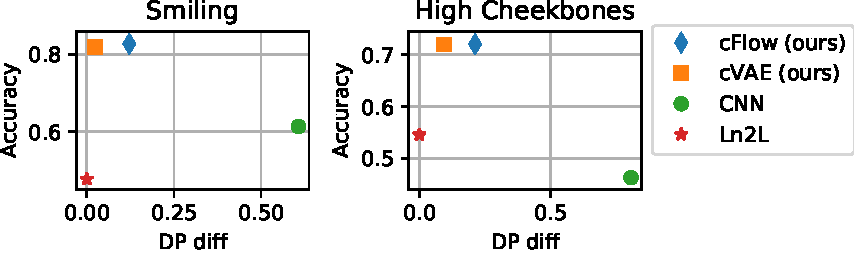
\includegraphics[width=0.7\textwidth]{nifr/Figures/nosinn_celeba.pdf}
    \caption{
        Performance of our model for different targets (mixing factor $\eta=0$).
        Left: \emph{Smiling} as target, right: \emph{high cheekbones}.
        \emph{DP diff} measures fairness with respect to demographic parity.
        A perfectly fair model has a \emph{DP diff} of 0.
    }%
    \label{fig:celeba-targets}
\end{figure}

\begin{figure}[tb]
    \centering
    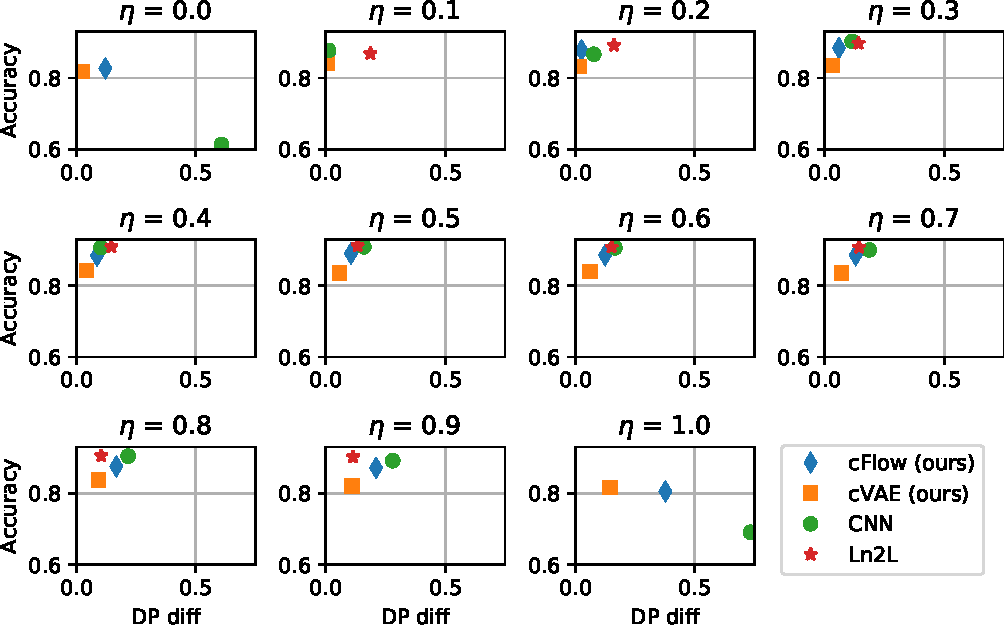
\includegraphics[width=0.85\textwidth]{nifr/Figures/nosinn_celeba_multiplot_all_landscape_Smiling.pdf}
    \caption{
        %
        Performance of our model for the target ``smiling'' for different mixing factors $\eta$.
        %
        \emph{DP diff} measures fairness with respect to demographic parity.
        %
        A perfectly fair model has a \emph{DP diff} of 0, thus the closer to top-left the better it
        is in terms of we accuracy-fairness trade-off.
        %
        Only values $\eta=0$ and $\eta=1$ correspond to the scenario of a strongly biased training
        set.
        %
        The results for $0.1\leq \eta\leq 0.9$ are to confirm that our model does not harm
        performance for non-biased training sets.
    }%
    \label{fig:celeba-multiplot}
\end{figure}
%
\subsection{Synthesising Dataset Bias}
%
For our experiments, we require a training set that exhibits a strong spurious correlation,
together with a test set that does not.
%
For cMNIST, this is easily satisfied as we have complete control over the data generation process.
%
For CelebA and  UCI Adult, on the other hand, we have to generate the split from the existing data.
%
To this end, we first set aside a randomly selected portion of the dataset from which to sample the
biased dataset.
%
The resulting portion is then split further into two parts: one in which \( (s=-1 \land y=-1) \lor
(s=+1 \land y=+1) \) holds true for all samples, call this part \( \mathcal{D}_{eq} \), and the
other part, call it \( \mathcal{D}_{opp} \), which contains the remaining samples.
%
To investigate the behaviour at different levels of correlation, we mix these two subsets according
to a mixing factor \( \eta \).
%
For $\eta \leq \tfrac{1}{2}$, we combine (all of) $\mathcal{D}_{eq}$ with a fraction of $2\eta$
from $\mathcal{D}_{opp}$.
%
For $\eta > \tfrac{1}{2}$, we combine (all of) $\mathcal{D}_{opp}$ and a fraction of $2(1 -\eta)$
from $\mathcal{D}_{eq}$.
%
Thus, for $\eta=0$, the biased dataset is just $\mathcal{D}_{eq}$, for $\eta=1$ it is just
$\mathcal{D}_{opp}$ and for $\eta=\tfrac{1}{2}$ the biased dataset is an ordinary subset of the
whole data. The test set is simply the data remaining from the initial split.
%
\subsection{Evaluation protocol}
%
We evaluate our results in terms of accuracy and fairness. A model that perfectly decouples its
predictions from $s$ will achieve near-uniform accuracy across all biasing-levels. 
%
For binary $s$/$y$ we quantify the fairness of a classifier's predictions using \emph{demographic
parity} (DP): the  absolute difference in the probability  of a positive prediction for each
sensitive group.

\begin{figure}[tb]
    \centering
    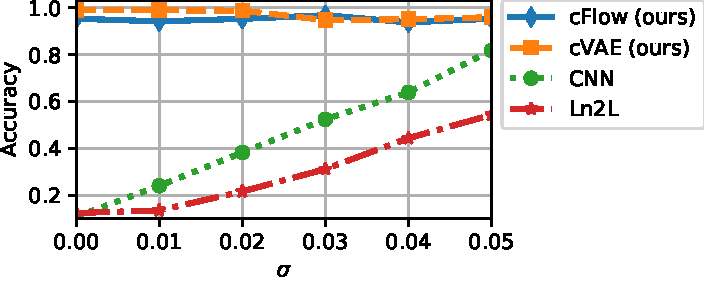
\includegraphics[width=0.7\textwidth]{nifr/Figures/cmnist_new_no_hgr.pdf}
    \caption{
        Accuracy of our approach in comparison with other baseline models on the cMNIST dataset,
        for different standard deviations ($\sigma$) for the colour sampling.
    }%
    \label{fig:cmnist_chart}
\end{figure}

\begin{figure*}[!htb]
    \centering
    \subfloat[Samples from the cMNIST training set, $\sigma=0$.]{%
        \scalebox{0.3}{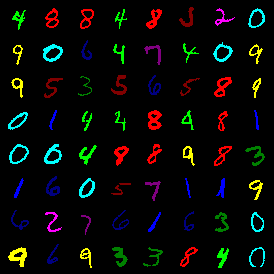
\includegraphics[width=\textwidth]{nifr/Images/cmnist/cflow_original_task_x_scale_0.png}}%
        \label{fig:cflow_cmnist_task_train}
    }
    \hfill
    \subfloat[$x_u$ null-samples from the \ac{cFlow} model.]{%
        \scalebox{0.3}{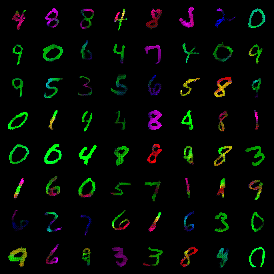
\includegraphics[width=\textwidth]{nifr/Images/cmnist/cflow_task_xy_scale_0.png}}%
        \label{fig:cflow_cmnist_y}
    }
    \hfill
    \subfloat[$x_b$ null-samples from the \ac{cFlow} model.]{%
        \scalebox{0.3}{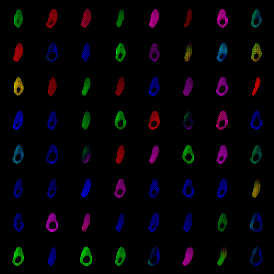
\includegraphics[width=\textwidth]{nifr/Images/cmnist/cflow_task_xs_scale_0.png}}%
        \label{fig:cflow_cmnist_s}
    }
    \caption{
        %
        Sample images from the coloured MNIST dataset problem with $10$ predefined mean colours.
        %
        (a): Images from the spuriously correlated subpopulation where colour is a reliable signal
        of the digit class-label.
        %
        (b-c): Results of running our approach realised with \ac{cFlow} on the cMNIST dataset.
        %
        The model learns to retain the shape of the digit while removing the relationship with
        colour.
        %
        A downstream classifier is now less prone to exploiting correlations between colour and the
        digit label class.
        %
    }\label{fig:cmnist}
\end{figure*}
%
\subsection{Experimental results}
%
We report the results from two image datasets. cMNIST, a synthetic dataset, is a good starting
point for evaluating our model due to the direct control we have over the biasing. 
%
CelebA, on the other hand, is a more practical and challenging example.
%
We also test our method on a tabular dataset, the Adult dataset.
%
\paragraph{cMNIST.}
%
The coloured MNIST (cMNIST) dataset is a variant of the MNIST dataset in which the digits are
coloured.
%
In the training set, the colours have a one-to-one correspondence with the digit class.
%
In the test set (and the representative set), colours are assigned randomly.
%
The colours are drawn from Gaussians with 10 different means.
%
We follow the colourisation procedure outlined by~\citet{kim2019learning}, with the mean colour
values selected so as to be maximally dispersed.
%
The full list of such values can be found in \S\ref{sec:color-details}.
%
We produce multiple variants of the cMNIST dataset corresponding to different standard deviations
$\sigma$ for the colour sampling: $\sigma \in \{0.00, 0.01, ..., 0.05 \}$.

For this specific dataset, we can establish an additional baseline by simply grey-scaling the
dataset which only leaves the luminosity as spurious information.
%
We also evaluate the model, with all the associated hyperparameters, from~\citet{kim2019learning}.
%
The only difference between the setups is the dataset creation, including the range of \(\sigma\)
values we consider.
%
Our versions of the dataset, on the whole, exhibit much stronger colour bias, to the point of the
mapping the digit's colour and class being bijective. 
%
Fig.~\ref{fig:cmnist_chart} shows that the model significantly underperforms even the na\"ive
baseline, aside from at \(\sigma = 0\), where they are at parity.
%
\corr{
%
Ln2L relies upon adversarial \ac{MI}-minimisation in the fashion of \citet{ganin2016domain}; we
conjecture that the sub-\ac{CNN} performance of Ln2L is consequent of the optimum of this objective
connoting invariance to both the digit and colour, as one may serve as an effective (with degree
scaling inversely with \(\sigma\)) for the other for both the classifier and the adversary, in
absence of partially-unlabelled data to decouple the attributes.
%
We would also expect invariance is also expected of the \ac{CNN} as a by-product of the excessive
variance to colour (that is to say, colour being a shortcut means that digit-information is
redundant, albeit -- importantly -- not deliberately excised) and the results indicate an
increasing noise-level alone more effectively breaks this than the aforementioned,
explicitly-enforced invariance (which is itself subject to noise, in addition with the predictive
streams) in tandem with it.
%
This degenerate behaviour of Ln2L may be attenuated with more judicious choice of pre-factor on
said \ac{MI}-minimisation term, though the problem hyperparameter selection for \ac{DG} problems is
challenging in its own right \citep{gulrajani2020search}; our method requires minimal consideration
in this respect due to non-conflicting objectives.
}
% CORRECTED: need more explanation of the figures here for me. Maybe can expand now you don't have
% page constraints. In particular comment on whey LN2L does so badly

Inspection of the null-samples shows that both the \ac{cVAE} and \ac{cFlow} model succeed in
removing almost all colour information, which is supported quantitatively by
Fig.~\ref{fig:cmnist_chart}, and qualitatively by Fig.~\ref{fig:cmnist}. 
%
While the \ac{cVAE} outperforms \ac{cFlow} marginally at low \(\sigma\) values, performance degrades
%rapidly
as this increases. 
%
This highlights the problems with the conditional decoder we anticipated in \S\ref{conddec}. 
%
The lower $\sigma$, and therefore the variation in sampled colour, is, the more reliably the $s$
label, corresponding to the mean of RGB distribution, encodes information about the colour. 
%
For higher $\sigma$ values, the sampled colours can deviate far from the mean and so the encoder
must incorporate information about $s$ into its representation if it is to minimise the
reconstruction loss. \ac{cFlow}, on the other hand, is consistent across $\sigma$ values.
%
\paragraph{CelebA.}
%
To evaluate the effectiveness of our framework on real-world image data we use the CelebA
dataset~\citep{liu2015faceattributes}, consisting of 202,599 celebrity images. 
%
These images are annotated with various binary physical  attributes, including ``gender'', ``hair
colour'', ``young'', etc., from which we select our sensitive and target attributes. 
%
The images are centre cropped and resized to $64\times64$, as is standard practice. 
%
For our experiments, we designate ``gender'' as the sensitive attribute, and ``smiling'' and ``high
cheekbones'' as target attributes. 
%
We chose gender as the sensitive attribute as it a common sensitive attribute in the fairness
literature. 
%
For the target attributes, we chose attributes that are harder to learn than gender and which do
not correlate too strongly with gender in the dataset (``wearing lipstick'' for example being an
attribute too closely correlated with gender).
%
The model is trained on the representative set (normal subset of CelebA) and is then used to encode
the artificially biased training set and the test set. The results for the most strongly biased
training set ($\eta=0$) can be found in Fig.~\ref{fig:celeba-targets}. Our method outperforms the
baselines in accuracy and fairness.

\begin{figure*}[tb]
  \centering
  \subfloat[Original images.]{%
      \scalebox{0.3}{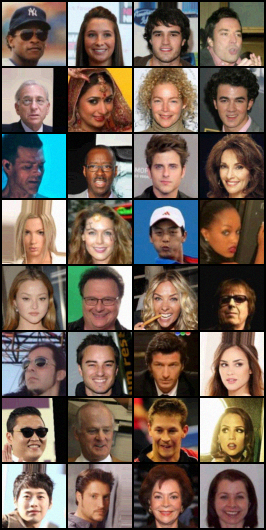
\includegraphics[width=\textwidth]{nifr/Images/celeba/train_original_x_2.png}}%
      \label{fig:cflow_celeba_original_x}
  }
  \hfill
  \subfloat[$\bm{x}_u$ null-samples from the cFlow model.]{%
      \scalebox{0.3}{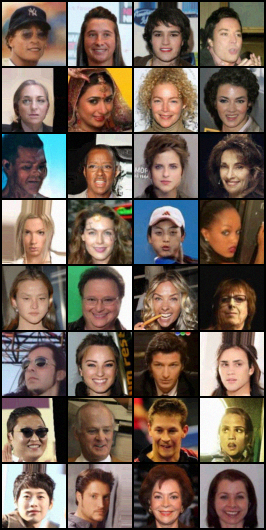
\includegraphics[width=\textwidth]{nifr/Images/celeba/train_reconstruction_y_2.png}}%
      \label{fig:cflow_celeba_recon_y}
  }
  \hfill
  \subfloat[$\bm{x}_b$ null-samples from the cFlow model.]{%
      \scalebox{0.3}{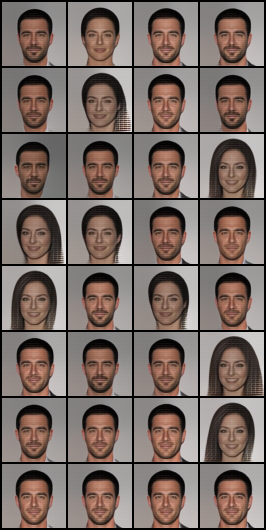
\includegraphics[width=\textwidth]{nifr/Images/celeba/train_reconstruction_s_2.png}}%
      \label{fig:cflow_celeba_recon_s}
  }
  \caption{
      CelebA null-samples learned by our \ac{cFlow} model, with gender as the sensitive attribute.
      %
      (a) The original, untransformed samples from the CelebA dataset
    %
      (b) Reconstructions using only information unrelated to $s$.
    %
      (c) Reconstruction using only information related to $\neg s$.
    %
      The model learns to disentangle gender from the non-gender related information.
      %
      Note that some attributes like skin tone seem to change along with gender due to the
      correlation between the attributes.
    %
      This is especially visible in images (1,1) and (3,2). Only because our representations are
      produced in the data-domain can we easily spot such instances of entanglement.
  }%
  \label{fig:celeba_cflow}
\end{figure*}
%
We also assess performance for different mixing factors ($\eta$) which correspond to varying
degrees of bias in the training set (see Fig.~\ref{fig:celeba-multiplot}).
%
This is to verify that the model does not \emph{harm} performance when there is not much bias in
the training set.
%
For these experiments, the model is trained once on the representative set and is then used to
encode different training sets.
%
The results show that for the intermediate values of $\eta$, our model incurs a small penalty in
terms of accuracy, but at the same time makes the results \emph{fairer} (corresponding to an
accuracy-fairness trade-off). 
%
Qualitative results can be found in Fig.~\ref{fig:celeba_cflow} (images from \ac{cVAE} can be found
in \S\ref{sec:qual-results-celeba}).

To show that our method can handle multinomial, as well as binary, sensitive attributes, we also
conduct experiments with $s=\textrm{hair colour}$ as a ternary attribute (``Blonde'', ``Black'',
``Brown''), excluding ``Red'' because of the paucity of samples and the noisiness of their labels.
%
The results for these experiments can be found in \S\ref{sec:additional-results}.

\begin{figure}[tb]
  \centering
  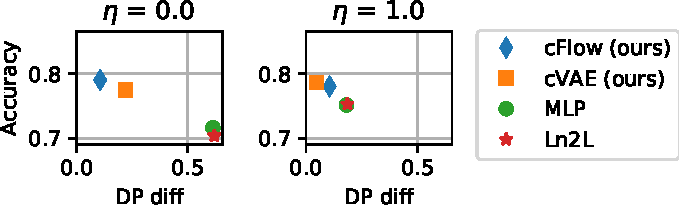
\includegraphics[width=0.6\textwidth]{nifr/Figures/nosinn_adult_multiplot_mini_diff.pdf}
  \caption{
      Results for the \textsc{Adult} dataset.
      The $x$-axis corresponds to the difference in positive rates.
      An ideal result would occupy the \textsc{top-left}.
  }%
  \label{fig:adult-chart}
\end{figure}
% \end{wrapfigure}

\paragraph{Results for the UCI Adult dataset.}
%
The UCI Adult dataset consists of census data and is commonly used to evaluate models focused on
\acl{AF}.
%
Following convention, we designate ``gender'' as the sensitive attribute $s$ and whether an
individual's salary is \$50,000 or greater as $y$.
%
We show the performance of our approach in comparison to baseline approaches in Fig.
\ref{fig:adult-chart}.
%
We evaluate the performance of all models for mixing factors ($\eta$) $0$ and $1$. 
%
Results shown in Fig. \ref{fig:adult-chart} show that we match or exceed the baseline.
%
In terms of fairness metrics, our approach generally outperforms the baseline models for both of
$\eta$.
%
Detailed results can be found in \S\ref{sec:additional-results}.

We also did experiments to show that the encoder transfers to other tasks. 
%
These transfer-learning experiments can be found in \S\ref{sec:transfer-learning}.


\section{Conclusion}\label{sec:nifr-conclusion}
%
We have proposed a general and straightforward framework for producing invariant representations,
under the assumption that a representative but partially-labelled \emph{representative} set is
available. 
%
Training consists of two stages: an encoder is first trained on the representative set to produce a
representation that is invariant to a designated spurious feature. 
%
This is then used as input for a downstream task-classifier, the training data for which might
exhibit extreme bias with respect to that feature. 
%
We train both a \acs{VAE}- and \acs{INN}-based model according to this procedure, and show that the
latter is particularly well-suited to this setting due to its losslessness. 
%
The design of the models allows for representations that are in the data domain and therefore
exhibit meaningful invariances. 
%
We characterise this for synthetic as well as real-world datasets for which we develop a method for
simulating sampling bias.
%

% \section*{Acknowledgements}
% %
% This work was in part funded by the European Research Council under the ERC grant agreement no.
% 851538. We are grateful to NVIDIA for donating GPUs.

\newpage
\section{Appendix}\label{sec:nifr-appendix}
%
\subsection{Model Architectures}
%
\label{sec:architectures}
%
\noindent For both cMNIST and CelebA we parametrise the coupling layers with the same convolutional
architecture as in \citet{KinDha18}, consisting of $3$ convolutional layers each with $512$ filters
of, in order, sizes $3\times3$, $1\times1$, and $3\times3$. 
%
Following \citet{ardizzone2019guided}, we Xavier initialise all but the last convolutional layer of
the $s$ and $t$ sub-networks which itself is zero-initialised so that the coupling layers begin by
performing an identity transform. 
%
We use a Glow-like architecture \citep{KinDha18} (affine coupling layers together with
chequerboard reshaping and invertible $1\times1$ convolutions) for the convolutional INNs. 
%
Table \ref{tab:inn_architectures} summarises the INN architectures used for each dataset.

For the image datasets each level of the \ac{cVAE} encoder consists of two gated convolutional layers
\citep{van2016conditional} with ReLU activation. 
%
At each subsequent level, the number of filters is doubled, starting with an initial value 32 and
64 in the case of CelebA and cMNIST respectively. 
%
In the case of the Adult dataset, we use an encoder with one fully-connected hidden layer of width
$35$, followed by SeLU activation \citep{klambauer2017self}. 
%
For both cMNIST and CelebA, we downsample to a feature map with spatial dimensions $8\times8$, but
with $3$ and $16$ channels respectively. 
%
For the Adult dataset, the encoding is a vector of size $35$. 
%
The output layer specifies both the parameters (mean and variance) of the representation's
distribution. 
%
In all cases the KL-divergence is computed with respect to a standard isotropic Gaussian prior. 
%
Details of the encoder architectures can be found in table \ref{tab:vae_architectures}. 
%
The loss pre-factors were sampled from a logarithmic scale; without proper balancing the networks
can exhibit instability, especially during the early stages of training.

\begin{table}[tp]
\caption{INN architecture used for each dataset.}
\label{tab:inn_architectures}
\centering
\begin{tabular}{lllll}
\toprule
Dataset & Levels & Level depth & Coupl. chan. & Input to discr. \\ \midrule
UCI Adult                   & 1      & 1     & 35       & Null-samples       \\
cMNIST                      & 3      & 16     & 512      & Encodings               \\
CelebA                      & 3      & 32     & 512      & Encodings        \\ \bottomrule
\end{tabular}
\end{table}

\begin{table}[tp]
\caption{
    \ac{cVAE} encoder architecture used for each dataset. The decoder architecture in each case mirrors that
of its encoder counterpart through use of transposed convolutions. For the adult dataset we apply
$\ell_2$ and cross-entropy losses to the reconstructions of the continuous features and discrete
features, respectively. }
\label{tab:vae_architectures}
\centering
\begin{tabular}{lllll}
\toprule
Dataset   & Initial channels & Levels & $\beta$ & Recon. loss \\
\midrule
UCI Adult & 35               & --     & 0       & $\ell_2$ + CE\\
cMNIST    & 32               & 4      & 0.01    & $\ell_2$ \\
CelebA    & 32               & 5      & 1       & $\ell_1$ \\ 
\bottomrule
\end{tabular}
\end{table}
%
\subsection{Additional results}\label{sec:additional-results}
%
\paragraph{Detailed results for UCI Adult dataset.}
%
This census data is commonly used to evaluate models focused on algorithmic fairness. 
%
Following convention, we designate ``gender'' as the $s$ and whether an individual's salary is
\$50,000 or greater as $y$. 
%
We show the performance of our approach in comparison to baseline approaches in
\figref{fig:big-adult-chart}. 
%
We evaluate the performance of all models for mixing factors ($\eta$) of value \( \{0, 0.1, \dots,
1\} \). 
%
Results shown in \figref{fig:big-adult-chart} show that while our model fails to surpass the
baseline models in terms of accuracy for the balanced case (and those close to it), we match or
exceed the baseline as $\eta $ moves the dataset to a more imbalanced setting. 
%
In terms of fairness metrics,  our approach generally outperforms the baseline models regardless of
$\eta$.

\begin{figure}[htb]
  \centering
  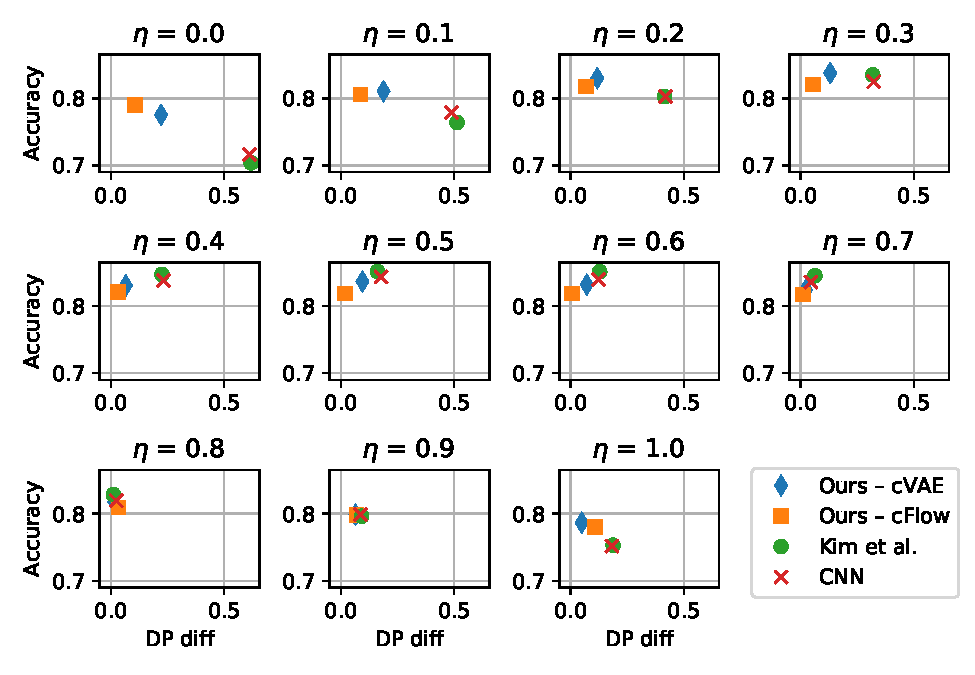
\includegraphics[width=0.85\textwidth]{nifr/Figures/nosinn_adult_multiplot_all_landscape_diff.pdf}
  \caption{
      Results for the \textsc{Adult} dataset.
      The $x$-axis corresponds to the difference in positive rates.
      An ideal result would occupy the \textsc{top-left}.
  }%
  \label{fig:big-adult-chart}
\end{figure}
\begin{figure}[htb]
    \centering
    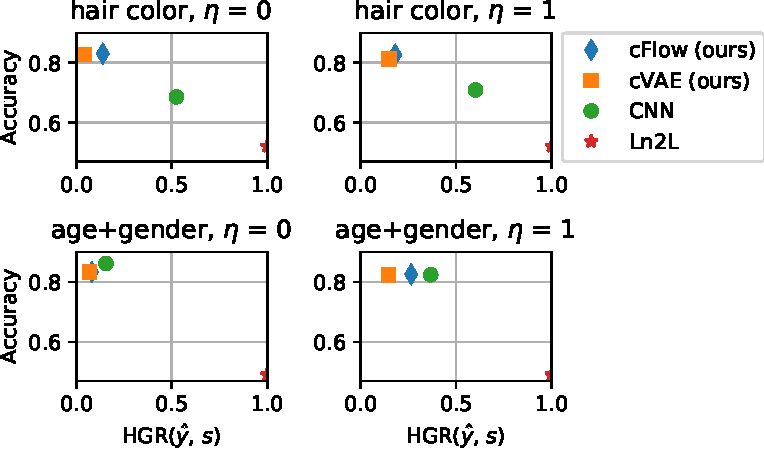
\includegraphics[width=0.7\textwidth]{nifr/Figures/celeba_multi_s.pdf}
    \caption{
        For \emph{hair colour}, $s$ takes on the values Blond, Brown and Black. For
        \emph{age+gender}, $s$ takes on the values Young/Female, Young/Male, Old/Female and
        Old/Male.
    }%
    \label{fig:multi-s}
\end{figure}
%
\paragraph{Multinomial sensitive attributes.}
%
In addition to binary sensitive attribute $s$, we also investigate multinomial $s$ in the CelebA
dataset. 
%
First, we do experiments with hair colour, where $s$ has three possible values: blond hair, brown
hair and black hair. 
%
The other experiment is with a combination of age and gender, where $s$ has four possible values,
each of which is a combination of a gender and an age: Young/Female, Young/Male, Old/Female and
Old/Male. 
%
To evaluate the fairness for multinomial $s$, we use \acl{HGRMC} (\acs{HGRMC},
\citep{mary2019fairness}), defined on the domain $[0, 1]$ and yielding \( \text{HGR}(Y,S)=0 \) iff
$Y \perp S$, \(1\) if there is a deterministic mapping between the variables. 
%
Results can be found in Fig.~\ref{fig:multi-s}.\\

\begin{table}[tp]
\caption{Results on the CelebA dataset with different sizes of $z_b$.}
    \label{tab:zs-ablation}
    \centering
\begin{tabular}{l@{\extracolsep{1cm}}lrr}
\toprule
 $|z_b|$ & $|z_b|/|z|$ &  Accuracy &   DP diff \\
\midrule
          1 &             0.0082\% &  0.60 &  0.63 \\
          3 &             0.0245\% &  0.60 &  0.63 \\
          5 &             0.0410\% &  0.84 &  0.12 \\
         10 &             0.0820\% &  0.84 &  0.12 \\
         30 &             0.2442\% &  0.74 &  0.23 \\
         50 &             0.4070\% &  0.68 &  0.27 \\
\bottomrule
\end{tabular}
\end{table}
\noindent\textsc{Investigation into the size of $z_b$.}
\;\; In the \ac{cFlow} model, the size of $z_b$ is an important hyperparameter which can affect the
result significantly.
%
Here we investigate the sensitivity of the model to the choice of $z_b$ size.
Table~\ref{tab:zs-ablation} shows accuracy and fairness (as measured by \emph{DP diff}) for
different sizes of $z_b$. 
%
The results show that both too large and too small $z_b$ is detrimental. 
%
However, they also show that the model is not overly sensitive to this parameter: both sizes 5 and
10 achieve nearly identical results.

\begin{table}[tbp]
    \caption{
        Additional fairness metrics for the experiments on the CelebA dataset
        (Fig.~\ref{fig:celeba-multiplot} from the main text). \emph{TPR diff.}\ refers to the
        difference in true positive rate. \emph{TNR diff.}\ refers to the difference in true
        negative rate. \textsc{Left:} $\eta = 0$. \textsc{Right:} $\eta=1$.
    }
    \label{tab:my_label}
    \resizebox{.49\textwidth}{!}{
    \begin{tabular}{lrrrr}
\toprule
     Method &  Accuracy &  DP diff &  TPR diff &  TNR diff \\
\midrule
      cFlow &      0.83 &     0.10 &      0.15 &      0.25 \\
       cVAE &      0.82 &     0.05 &      0.09 &      0.18 \\
        CNN &      0.61 &     0.63 &      0.70 &      0.64 \\
 Ln2L &      0.52 &     0.00 &      0.00 &      0.00 \\
\bottomrule
\end{tabular}}
\hfill
\resizebox{.49\textwidth}{!}{
\begin{tabular}{lrrrr}
\toprule
     Method &  Accuracy &  DP diff &  TPR diff &  TNR diff \\
\midrule
      cFlow &      0.82 &     0.33 &      0.28 &      0.21 \\
       cVAE &      0.81 &     0.16 &      0.10 &      0.05 \\
        CNN &      0.67 &     0.75 &      0.66 &      0.76 \\
Ln2L &      0.51 &     0.08 &      0.06 &      0.09 \\
\bottomrule
\end{tabular}}
\end{table}
\paragraph{Additional fairness metrics.}
%
In addition to \emph{DP diff}, we report here the result from other fairness measures. 
%
These results are from the same setup as those reported in the main paper. 
%
We report the difference in \acp{TPR} between the two groups (male and female), which corresponds
to a measure of \acf{EqOd}, and the difference in \acp{TNR} between the two groups.

\subsection{Optimisation Details}\label{sec:nifr-optimisation-details}
%
\noindent All our models were trained using the RAdam optimiser \citep{liu2019variance} with
learning rates $3\times10^{-4}$ and $1\times10^{-3}$ for the encoder/discriminator pair and
classifier respectively. 
%
A batch size of 128 was used for all experiments.

We now detail the optimisation settings, including the choice of adversary, specific to each
dataset.
%
Details of the \ac{cVAE} and \ac{cFlow} architectures can be found in table \ref{tab:vae_architectures} and
table \ref{tab:inn_architectures}, respectively.

\paragraph{UCI Adult.}
%
For this dataset our experiment benefited from using null-samples as inputs to the adversary of the
\ac{cFlow} model. 
%
Unlike for the image datasets, we found a single adversary to be sufficient. 
%
This was realised as a \acf{MLP} with one hidden layer, 256 units wide. 
%
The \ac{INN} performs a bijection of the form $f: \mathbb{R}^n \rightarrow \mathbb{R}^n$. 
%
However, the adult dataset is composed of mostly discrete (binary/categorical) features. 
%
To achieve good performance, we found it necessary to first pre-process the inputs with a
pretrained autoencoder, using its encodings as the input to the \ac{cFlow} model, as well as to the
adversary. 
%
The learned representations were evaluated with a logistic regression model from scikit-learn
\citep{scikit-learn}, using the standard settings. 
%
All baseline models were trained for 200 epochs. 
%
The Ln2L \citep{kim2019learning} and \ac{MLP} baselines share the architecture of the \ac{cVAE}'s
encoder, only with a classification layer affixed.

\paragraph{Coloured MNIST.} Each level of the architecture used for the downstream classifier and
na\"ive baseline alike consists of two convolutional layers, each with kernel size 3 and followed
by Batch Norm \citep{ioffe2015batch} and ReLU activation. 
%
For the Ln2L baseline, we use an a setup identical to that described in \citet{kim2019learning}. 
%
Each level has twice the number of filters in its convolutional layer and half the spatial input
dimensions as the last. 
%
The original input is downsampled to the point of the output being reduced to a vector, to which a
fully-connected classification layer is applied.

To allow for an additional level in the \ac{INN} (the downsampling operations requiring the number
of spatial dimensions to be even), the data was zero-padded to a size of $32\times32$. 
%
The \ac{cVAE} and \ac{cFlow} models were trained for 50 and 200 epochs respectively, using $\ell_2$
reconstruction loss for the former. The downstream classifier and all baselines were trained for 40
epochs. 
%
For both of our models, an ensemble of 5 adversaries was applied to the encodings, with each member
taking the form of a fully-connected ResNet, 2 blocks in depth, with SeLU activation
\citep{klambauer2017self}.
%
The adversaries were reinitialised independently with probability $0.2$ at the end of each epoch.
%
While the adversaries could equally well take  null-samples as input, as done for the Adult
dataset, doing so requires the performing of both forward and inverse passes each iteration, which,
for the convolutional \acp{INN} of the depths we require for the image datasets, introduces a large
computational overhead, while also showing to be the less stable of the two approaches in our
preliminary experiments.

\paragraph{CelebA.} The downstream classifier and na\"ive baseline take the same form as described
above for cMNIST, but with an additional level with 32 filters in each of its convolutions at the
top of the network. 
%
For this dataset we adapt the Ln2L model by simply considering it as an augmentation the na\"ive
baseline's objective function, with the entropy loss applied to the output of the final
convolutional layer. 
%
These models were again trained for 40 epochs, which we found to be sufficient for convergence for
the tasks in question. 
%
The \ac{cVAE} and \ac{cFlow} models were respectively trained for 100 epochs and 30 epochs, using $\ell_1$
reconstruction loss for the former. 
%
Compared with cMNIST, the size of the adversarial ensemble was increased to 10, the
reinitialisation probability to 0.33, but no changes were made to the architectures of its members.

\paragraph{The Pitfalls of Adversarial Training.}
%
Adversarial learning has become one of the go-to methods for enforcing invariance in fair
representation learning \citep{ganin2016domain} with \ac{MMD} \citep{louizos2016variational} and HSIC
\citep{QuaShaTho19}, being popular non-parametric alternatives. 
%
\citet{ganin2016domain} proposed \acf{AdvL} for \acf{DA} problems, with
\citet{edwards2016censoring} soon after making this and learning a representation promoting
\ac{DP}. 
%
The adversarial approach carries the benefits of being both efficient and scalable to multi-class
categorical variables, which many sensitive attributes are in practice, whereas the non-parametric
methods only permit pair-wise comparison.

However, when realised as a neural network, the adversary is both sensitive to the values of the
inputs as well as their ordering (though exchangeable architectures, such as \citet{zaheer2017deep}
do exist, but which sacrifice expressiveness). 
%
Thus, it can happen that the representation learner optimises for the surrogate objective of
eluding the adversary rather than the real objective of expelling $s$-related information. 
%
Moreover, the non-stationarity of the dynamics can lead to cyclic equilibria, irrespective of the
capacity of the adversary.

When working with a partitioned latent space, this behaviour can be averted by instead encouraging
$z_b$ to be predictive of $s$, acting as a kind of information ``sink'', as in \citet{JacSmeOya18}.
%
However, this does not have the guarantee of making $z_u$ invariant to $s$ - there are often many
indicators for $s$, not all of which are needed to predict the label perfectly. 
%
Training the network to convergence before taking each gradient step with the representation
learner is one way one to attempt to tame the unstable minimax dynamics \citep{feng2019learning}. 
%
However, this does not prevent the emergence of the aforementioned cyclicity.

We try to mitigate the aforementioned degeneracies by maintaining a diverse set of adversaries, as
has shown to be effective for GAN training \citep{durugkar2016generative}, and by decorrelating the
individual trajectories by intermittently re-initialising them with some small probability
following each iteration.

\paragraph{Tuning the Partition Sizes.}
%
There are several ways of ensuring that the size of $z_b$ is sufficient to capture all s
dependencies, but minimal enough that information unrelated to s is maximally preserved We adopt
the straightforward search strategy of, starting from some initial guess, calibrating the value
according to accuracy attained by a classifier trained to predict $s$ from $z_b$ on a held-out
subset of the representative set, which is measured whenever the adversarial loss plateaus. 
%
If the accuracy is above chance level then that suggests the size of the $z_b$ partition, $|z_b|$,
needs to be increased to accommodate more information about $s$. 
%
If the accuracy is found to be at chance level then are two possibilities: 
%
1) $|z_b|$ is already optimal; 
%
2) $|z_b|$ is large enough that it fully contains both information $s$ as well as that of a portion
of $y$. 
%
If the former is true, then perturbations around the current value allow us to confirm this; if the
latter is true then decreasing the value was indeed the correct decision.

\begin{table}[tp]
\caption{
Mean RGB values (in practice normalised to $[0, 1]$) parametrising the Multivariate Gaussian
distributions from which each digit's colour is sampled in the biased (training) dataset. 
%
In the representative and test sets,  the colour of each digit is sampled from one of the specified
Gaussian distributions at random.
}
\label{tab:cmnist_rgb_values}
\centering
\begin{tabular}{l@{\extracolsep{1cm}}lll}
\toprule
Digit & Colour Name & Mean RGB      \\ \midrule
0     & Cyan        & (0, 255, 255) \\
1     & Blue        & (0, 0, 255)   \\
2     & Magenta     & (255, 0, 255) \\
3     & Green       & (0, 128, 0)   \\
4     & Lime        & (0, 255, 0)   \\
5     & Maroon      & (128, 0, 0)   \\
6     & Navy        & (0, 0, 128)   \\
7     & Purple      & (128, 0, 128) \\
8     & Red         & (255, 0, 0)   \\
9     & Yellow      & (255, 255, 0) \\ \bottomrule
\end{tabular}
\end{table}

\subsection{Synthesising Coloured MNIST}\label{sec:color-details}
\noindent We use a colourised version of MNIST as a controlled setting investigate learning from
biased data in the image domain. 
%
In the biased training set, each digit is assigned a unique mean RGB value parametrising the
multivariate Gaussian from which its colour is drawn. 
%
These values were chosen to be maximally dispersed across the 8-bit colour spectrum and are listed
in table \ref{tab:cmnist_rgb_values}. 
%
By adjusting the standard deviation, $\sigma$, of the Gaussians, we adjust the degree of bias in
the dataset. 
%
When $\sigma=0$, there is a perfect and noiseless correspondence between colour and digit class
which a classifier can exploit. 
%
The classifier can favour the learning of the low-level spurious feature over those higher level
features constituent of the digit's class. 
%
As the standard deviation increases, the sampled RGB values are permitted to drift further from the
mean, leading to overlap between the samples of the colour distributions and reducing their
reliability as indicators of the digit class. 
%
In the test and representative sets alike, however, the colour of each sample is sampled from one
of the 10 distributions randomly, such that colour can no longer be leveraged as a shortcut to
predicting the digit's class.

\subsection{Stabilising the Coupling layers}\label{sec:those-darn-coupling-layers}
%
\noindent Heuristically, we found that  applying an additional non-linear function to the scale
coefficient of the form
%
\begin{align}
  s = \sigma (f(u)) + 0.5
  \label{eq:heuristic-1}
\end{align}
%
greatly improved the stability of the affine coupling layers. 
%
Here, $\sigma$ is the logistic function, which we shift to be centred on 1 so that
zero-initialising $f$ results in the coupling layers initially performing an identity-mapping.

% \newpage
\begin{figure*}[tb]
  \centering
  \subfloat[Original images.]{%
      \scalebox{0.3}{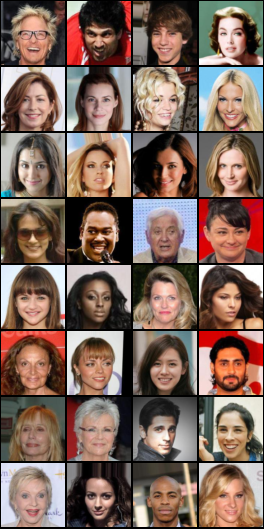
\includegraphics[width=\textwidth]{nifr/Images/celeba/vae_x_original.png}}%
      \label{fig:cvae_celeba_original_x}
  }
  \hfill
  \subfloat[$x_u$ null-samples generated by the \ac{cVAE} model.]{%
      \scalebox{0.3}{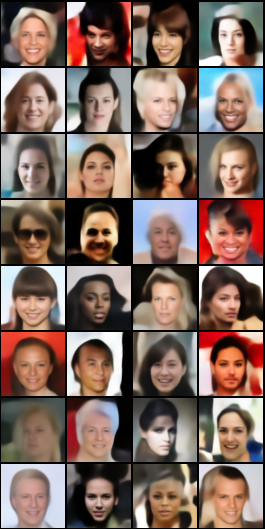
\includegraphics[width=\textwidth]{nifr/Images/celeba/vae_recon_y.png}}%
      \label{fig:cvae_celeba_recon_y}
  }
  \hfill
  \subfloat[$x_b$ null-samples generated by the \ac{cVAE} model.]{%
      \scalebox{0.3}{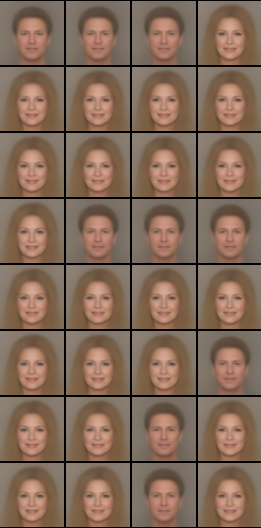
\includegraphics[width=\textwidth]{nifr/Images/celeba/vae_recon_s.png}}%
      \label{fig:cvae_celeba_recon_s}
  }
  \caption{
      CelebA null-samples learned by our \ac{cVAE} model, with gender as the sensitive attribute.
    %
    (a) The original, untransformed samples from the CelebA dataset
    %
    (b) Reconstructions using only information unrelated to $s$.
    %
    (c) Reconstruction using only information related to $\neg s$.
    %
    The model learns to disentangle gender from the non-gender related information. 
    %
    Compared with the \ac{cFlow} model, there is a severe degradation in reconstruction quality due to
    the model trying to simultaneously satisfy conflicting objectives.
    % Attributes such as \emph{make-up} and \emph{hair length} are also often modified in the
    % process due to inherent correlations between them and the sensitive attribute, which the
    % intepretability of our representations allows us to easily identify.
  }\label{fig:celeba_vae}
\end{figure*}

\begin{figure*}[tb]
  \centering
  \subfloat[Original images.]{%
      \scalebox{0.3}{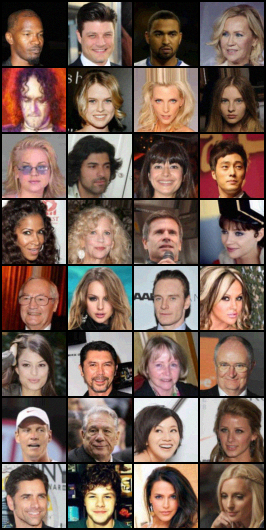
\includegraphics[width=\textwidth]{nifr/Images/celeba/cflow_original_x_suppmat.png}}%
      \label{fig:cflow_celeba_original_x_suppmat}
  }
  \hfill
  \subfloat[$x_u$ null-samples generated by the \ac{cFlow} model.]{%
      \scalebox{0.3}{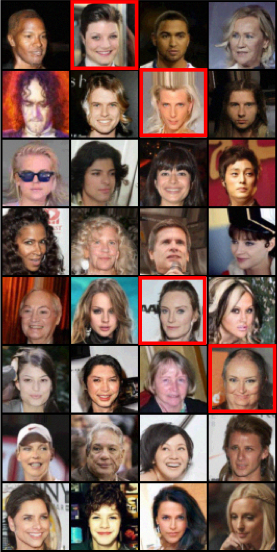
\includegraphics[width=\textwidth]{nifr/Images/celeba/cflow_xd_suppmat.png}}%
      \label{fig:cflow_celeba_recon_y_suppmt}
  }
  \hfill
  \subfloat[$\mathbf{x}_b$ null-samples generated by the \ac{cFlow} model.]{%
      \scalebox{0.3}{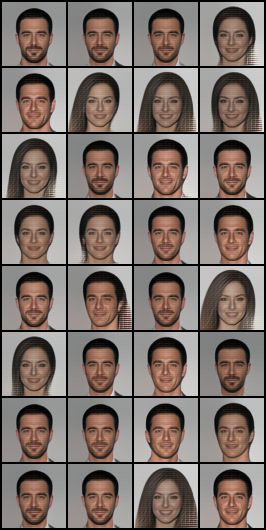
\includegraphics[width=\textwidth]{nifr/Images/celeba/cflow_xb_suppmat.png}}%
      \label{fig:cflow_celeba_recon_s_suppmat}
  }
  \caption{
      CelebA null-samples learned by our \ac{cFlow} model, with gender as the sensitive attribute.
    %
    (a) The original, untransformed samples from the CelebA dataset
    %
    (b) Reconstructions using only information unrelated to $s$.
    %
    (c) Reconstruction using only information related to $\neg s$.
    %
    The model learns to disentangle gender from the non-gender related information. 
    %
    Attributes such as \emph{make-up} and \emph{hair length} are also often modified in the process
    (prime examples framed with red) due to inherent correlations between them and the sensitive
    attribute, which the interpretability of our representations allows us to easily identify.
  }\label{fig:celeba_cflow_suppmat}
\end{figure*}

\subsection{Qualitative Results for CelebA}\label{sec:qual-results-celeba}
%
\noindent Learning a representation alongside its inverse mapping, be it approximate or exact,
enables us to probe the behaviour of the model that produced it, and any biases it may have
implicitly captured due to entanglement between the sensitive attribute and other attributes
present in the data. 
%
We highlight a few examples of such biases manifesting in the \ac{cFlow} model's CelebA null-samples in
Fig.~\ref{fig:celeba_cflow_suppmat}. 
%
In these cases, make-up and hair style have been inadvertently modified during the null-sampling
due to the tight correlation between these two attributes and the sensitive attribute, gender, to
which we had aimed to make our representations invariant. 
%
Additionally, in all highlighted images, the skin tone has changed: from male to gender-neutral,
the skin becomes lighter and from female to gender-neutral, the skin becomes darker; in the change
from male to gender-neutral, glasses are also often removed.
%
As the model cannot know that the label is meant to only refer to gender, and not to these other
(correlated) attributes, the links cannot be disentangled by the model.
%
However, the advantage of our method is that we can at least identify such biases due to the
interpretability that comes with the representations being in the data domain.

\begin{figure*}[htb]
  \centering
  \subfloat[Performance on cMNIST test data after pre-training on the mixed NIST dataset.]{
      \scalebox{0.6}{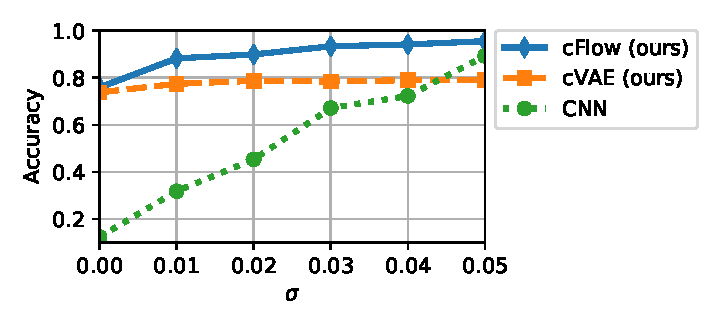
\includegraphics[width=\textwidth]{nifr/Figures/nosinn_cmnist_transfer.pdf}} \label{fig:cmnist-transfer}
  }
  %---
  \vspace{10pt}
 
  \subfloat[Test data input to the \ac{cFlow} model.]{%
      \scalebox{0.3}{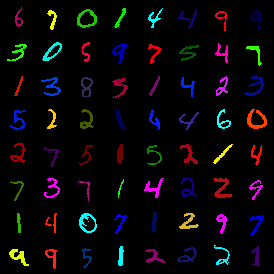
\includegraphics[width=\textwidth]{nifr/Images/cmnist/cflow_tl_original.png}}%
      \label{fig:cflow_tl_original}
  }
  ~~~
%   \hfill
  \subfloat[$x_u$ null-samples generated by the \ac{cFlow} model.]{%
      \scalebox{0.3}{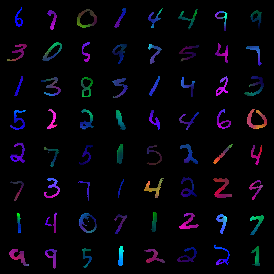
\includegraphics[width=\textwidth]{nifr/Images/cmnist/cflow_tl_xd.png}}%
      \label{fig:cflow_tl_xd}
  }
  
  \subfloat[Test data input to the \ac{cVAE} model.]{%
      \scalebox{0.3}{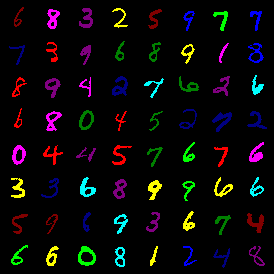
\includegraphics[width=\textwidth]{nifr/Images/cmnist/cvae_tl_original.png}}%
      \label{fig:cvae_tl_original}
  }
  ~~~
%   \hfill
  \subfloat[$x_u$ null-samples generated by the \ac{cVAE} model.]{%
      \scalebox{0.3}{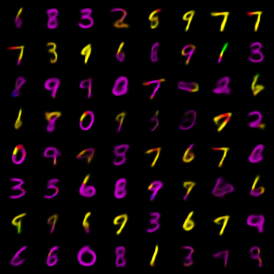
\includegraphics[width=\textwidth]{nifr/Images/cmnist/cvae_tl_xd.png}}%
      \label{fig:cvae_tl_xd}
  }
  \caption{
    Results for the transfer learning experiments in which the representative set consists of
    colourised samples from EMNIST, KMNIST, and FashionMNIST, while the downstream dataset remains
    as cMNIST. 
    %
    (a) Quantitative results for different $\sigma$-values. 
    %
    (b-c) Qualitative results for the \ac{cFlow} model. 
    %
    (d-e) Qualitative results for the \ac{cVAE} model. 
    %
    The qualitative results provide comparisons of the images before (left) and after (right)
    null-sampling. 
    %
    Note that for some of the \ac{cVAE} samples, the clarity of the digits has clearly changed due to
    null-sampling, serving as an explanation for the non-increasing downstream performance.
  }%
  \label{fig:cmnist-transfer-all}
  
\end{figure*}

\subsection{Transfer Learning}\label{sec:transfer-learning}
%
\noindent For our method, we require a representative set which follows the same distribution as
that observed during deployment. 
%
Such a representative set might not always be available. 
%
In such a scenario, we can resort to using a set that is merely \emph{similar} to that in the
deployment setting and leverage transfer learning.

%We argue that the inherent properties of INNs make them especially suitable for transfer learning.
One of the advantages of using an invertible architecture over conventional, \emph{surjective} ones
that we stressed in the main text is its \emph{losslessness}. 
%
Since the transformations are necessarily bijective, the information contained in the input can
never be destroyed, only redistributed. 
%
This makes such models particularly well-suited, in our minds, for transferring
learned invariances: even if the input is unfamiliar, no information should be lost when trying to
transform it. 
%
This works as long as only the information about $s$ ends up in the $z_b$ partition.
%
If $s$ takes a form similar to that which we pre-trained on, and can thus be correctly partitioned
in the latent space, by complement we have the information about $\neg s$ stored in the $z_u$
partition, without presupposing similarity to the $\neg s$ observed during pre-training.
%
\paragraph{Transferring from mixed-NIST to MNIST.}
%
We test our hypothesis by comparing the performance of the \ac{cFlow} and \ac{cVAE} models pre-trained on a
mixture of datasets belonging to the NIST family, colourised in the same way as cMNIST, while the
downstream train and test sets remain the same as in the original cMNIST experiments. 
%
Specifically, we create this representative set by sampling 24,000 images (to match the cardinality
of the original representative set) from EMNIST (letters only; \citealp{cohen2017emnist}),
Fashion\-MNIST~\citep{xiao2017fashion} and KMNIST~\citep{clanuwat2018deep}, in equal proportion. 
%
We use the same architectures for the \ac{cVAE} and \ac{cFlow} models as we did in the non-transfer learning
setting. 
%
In terms of hyperparameters, the only change made was to the KL-divergence's pre-factor, finding it
necessary to increase it to $1$ to guarantee stability.

The results for the range of $\sigma$ values are shown in Fig.~\ref{fig:cmnist-transfer}.
%
Unsurprisingly, the performance of both models suffers when the representative and test sets do not
completely correspond. 
%
However, the \ac{cFlow} model consistently outperforms the \ac{cVAE} model, with the gap increasing as the
bias decreases. 
%
Although some colour information is retained in the \ac{cFlow} null-samples, symptomatic of an imperfect
transfer, semantic information is almost entirely retained as well. 
%
Conversely, the \ac{cVAE} is very much flawed in this respect; as can be seen in the bottom row of
Fig.~\ref{fig:cmnist-transfer}, for some samples, semantic information is degraded to the point of
the digit's identity being altered. 
%
As a result of this semantic degradation, the performance of the downstream classifier is curtailed
by the noisiness of the digit's identity and is relatively unchanging across $\sigma$-values, in
contrast to the monotonic improvement of that achieved on the \ac{cFlow} null-samples.

% \begin{figure}
%   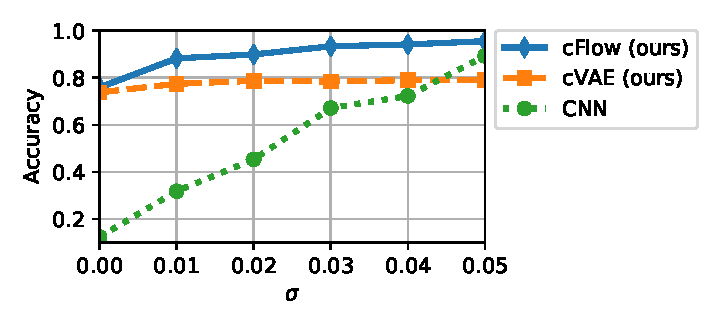
\includegraphics[width=0.6\textwidth]{nifr/Figures/nosinn_cmnist_transfer.pdf}
%   \caption{
%      Results for transfer learning experiments on cMNIST.
%   }%
%   \label{fig:cmnist-transfer}
% \end{figure}

% \clearpage

% \bibliographystyle{splncs04}
% \bibliography{references.bib}

% \end{appendix}

% \end{document}

\clearpage
\section{Authorial contributions}
%
{\renewcommand\labelitemi{}
%
\begin{itemize}
    %
    \item 
        %
        \textbf{T. Kehrenberg} conceived of the idea of using an INN combined with a
        representative set to learn an invariant representation in the face of spurious
        correlations, ran many of the experiments -- especially so in the initial stages -- and
        wrote much of the original text and code.
        %
    \item 
        %
        \textbf{I} wrote a significant part of the code (being responsible for several refactorings
        as part of the debugging process), the much of the text, helped crystallise the initial
        idea, ran many of the experiments, aided in experimental analysis, and developed much of
        the technical tricks needed to train the INN stably within the adversarial framework
        (grappling with the issues later elucidated by \citet{behrmann2021understanding}).
        %
    \item 
        %
        \textbf{O. Thomas} aided in writing the code, in running the experiments, partook in
        discussion and analysis of results, helped writing and formatting the paper, and served as
        an unwavering source of optimism.
        %
    \item
        %
        \textbf{N. Quadrianto} supervised the project, providing feedback on current progress and
        iterations of the paper and advising which directions to pursue.
        %
    %
\end{itemize}
%
}


%   \printbibliography
% \end{refsection}

% \begin{refsection}[okapi]
%   % ---------------------------------------------------------------------------------------
\chapter{Okapi: Generalising Better by Making Statistical Matches Match}\label{ch:okapi}
% ---------------------------------------------------------------------------------------
\textsc{Authors}:\\
Myles Bartlett$^1$, Sara Romiti$^1$, Viktoriia Sharmanska$^{1,2}$, and Novi Quadrianto$^{1,3,4}$ \\
\textsc{Affiliations}:\\
$^1$ Predictive Analytics Lab (PAL), University of Sussex, Brighton, UK\\
$^2$ Imperial College London \\
$^3$ BCAM Severo Ochoa Strategic Lab on Trustworthy Machine Learning \\
$^4$ Monash University, Indonesia \\
\textsc{Conference}:\;\;\textit{Neural Information Processing Systems} (NeurIPS), 2022 \\
% ---------------------------------------------------------------------------------------
\import{okapi}{commands.tex}
\import{okapi}{abstract.tex}
\import{okapi}{introduction.tex}
\import{okapi}{preliminaries.tex}
\import{okapi}{methodology.tex}
\import{okapi}{related_work.tex}
\import{okapi}{experiments.tex}
\import{okapi}{conclusion.tex}
\import{okapi}{ack.tex}
\newpage
\appendix
\import{okapi}{supplementary.tex}

%   \printbibliography
% \end{refsection}

\cleardoublepage
% \part{Conclusion}\label{pt:end}
% \chapter{Discussion and future work}\label{ch:conclusion}
In this thesis, I have presented three approaches for dealing with dataset bias.
The first one deals with a form of label bias and the other two with forms of sampling bias;
in both cases the bias is linked to a special attribute \(s\) of the data.
%
% mention again the main strengths of the presented methods
%
With the first approach, the user specifies target rates that can be used to tune the method to the desired outcome.
The method is flexible and easy to integrate with existing algorithms.
The second approach uses a partially-labelled representative set to learn an interpretable and invariant representation.
The user can directly observe in what way the data was changed to make it invariant
to the spurious correlation that is present in the training data.
The third approach in many ways builds upon the second one;
a set similar to the representative set is needed but there is no requirement for labels nor for balance of subgroups.
However, in the training set, the relationship between the class label \(y\) and subgroups \(s\) may not be
as close to a one-to-one mapping of \(y\) and \(s\) as in the second approach.
From these simple starting points, an invariant representation is learned
that can be used to train unbiased classifiers.

\section{data is bad}
Now, one possible objection here is:
if those datasets are of such poor quality,
then maybe we just should not train any \ac{ML} model on these and should not use them to make automated decisions?
While this question is mostly beyond the scope of this document, let me offer some thoughts on this:
It is true that even after the application of de-biasing techniques,
the resulting models still should not be fully trusted,
but they can still ease the burden of checking everything manually;
similar to an email spam filter which is not perfect, but still very useful.
Or, put another way, it is always important to check what the realistic alternative is;
we should not compare a model to a non-existing perfect ideal, but to the actual solution that would be used instead.
One could imagine a hybrid approach where an automated system makes preliminary decisions,
but random samples are reviewed by humans and decisions can always be challenged.
Ideally, the model itself would tell us about decisions it is uncertain about.

Moreover, two of the three methods presented in this thesis require access to (unlabelled) \emph{unbiased} data,
which is used during the training process.
The remaining method requires summary statistics of the unbiased target dataset.
So, the criticism that we are only learning from biased data does not apply here.
This should allow us to be more confident in the predictions produced by those methods,
because the methods learn from additional, unbiased information.

\section{resume previous text}

While this by no means covers \emph{all} possible biases,
it contributes to a growing literature that tries to tackle this problem.
One could ask if there is one method that is able to cover all possible dataset biases,
but I think there is a strong argument to be made that no general method can exist,
because it is, \eg, not possible to describe in general what is spurious information and what is relevant information.
Nevertheless, finding methods that are more generally applicable is a worthy goal.
One immediate avenue for future work is
the combination of label bias correction and sampling bias correction.
For example, it might be possible to leverage an unlabelled context set for correcting label bias as well.

There are also certain technical improvements that could be made.
In general, it would be desirable to have more theoretical bounds on performance.
This likely involves specifying the requirements for the algorithms more precisely.
% which is also useful information for potential users.
The method based on target labels would furthermore benefit from better-calibrated probability outputs.
\acf{GP} classifiers show generally good calibration,
but cannot be easily applied in domains where deep neural networks are used.
On the other hand, neural networks are known to be overconfident
\citep[especially when using ReLU activations;][]{hein2019relu},
so to apply the proposed method to images directly is not straightforward.
The other two proposed methods would benefit from improved adversarial training procedures.
Training these models is not straightforward as the losses have to be balanced
and in some cases, the update schedule needs to be changed.
Both the calibration of neural networks and the stability of adversarial training
are issues that are widely recognised in the \ac{ML} community,
so there is hope that progress will be made on these.

Another potential extension of this work is to extend it to other modalities.
The experiments were all performed on either tabular or image data
--- the reason predominantly being ease of visualisation ---
so working with audio (especially speech) or text could present new, interesting challenges.

Furthermore, as it currently stands,
the \ac{ML} practitioner has to know the bias in the data very well in order to choose a method to correct it.
It would be desirable to have a simple algorithm for deciding which method to use.
A related limitation is that the dataset bias considered in this thesis
is assumed to be linked to a special attribute \(s\).
While \(s\) can be very high-dimensional and is not limited to, say, binary attributes,
this nevertheless represents a restriction
that excludes large areas of dataset biases.

In any case, correcting dataset bias remains a challenging topic
and one that is increasingly relevant to today's machine learning applications.
Any cutting-edge \ac{ML} system will have to deal with imperfect data,
especially if the collected data is human-related.
The possible effects of these imperfections in the data are certainly highly undesirable:
a photo-tagging service might only work for a certain kind of person;
a speech recognition system might only work for a certain kind of dialect.
If, in these situations, sufficient representative (but unlabelled) data is available,
then the methods presented here can be used to try and correct the problem.

One area of machine learning that has recently seen increased interest is unsupervised learning,
and the latter two chapters make use of it to some degree.
The exciting promise of unsupervised learning in general is
that labour-intensive labelling is not needed and so vast amounts of existing, unlabelled data can be put to good use.
One could ask the question whether bias-correcting methods are still needed, with access to so much data.
It could be that, while the data is certainly not perfect,
there is so much of it that the biased parts ``cancel each other out''.
However, recent investigations of the GPT models \citep{radford2018improving,radford2019language,brown2020language} do not seem to support this \citep{khalifa2021distributional}.
One reason for this might be the way these models are trained at the moment:
they maximise the probability assigned to the next token.
Thus, such a model has to account for the wide array of human opinions and assign a non-zero probability to all of them.
So, when asked to summarise a text \citep{stiennon2020learning}, GPT does not give the \emph{best} summary;
rather, it gives a summary that an average person might have written.
However, with the help of a very high-quality labelled dataset (that was expensive to create),
GPT could be finetuned to actually produce very good summaries.
I suspect this pattern of learning the basics in an unsupervised fashion,
and then finetuning with high-quality labels, will continue in the future.
With these massive models,
it is, more than ever, crucial to build tools to make the biases within the models transparent.
Given the black-box nature of neural networks, this represents a major challenge.
% When examining these models trained on massive datasets through the lens of the dataset biases discussed in \chapref{ch:related-work},
% we encounter a novel problem:
% somewhere in the model,
% (an approximation of) the fundamental structures of reality are likely represented,
% but we cannot easily access this.

Finally, an important issue is the communication between human and machine.
The methods presented in this thesis have all strived to make it easy for human operators to understand what is going on:
the method in \chapref{ch:paper1} is configured with simple statistics;
the method in \chapref{ch:paper2} produces invariant images that can be inspected;
and the method in \chapref{ch:paper3} has the same capability
(though it is not part of the core functionality).
However, this is only a beginning.
It is still not easy to notice that a given dataset has problems,
and machines on their own cannot notice the problem,
because they do not (yet) have a complete understanding about what it is that humans care about;
human preferences are incredibly complex \citep{yudkowsky2011complex} and hard to predict for today's algorithms.
Thus, it is important that machines get feedback early and often,
to keep them aligned with human goals.
(The aforementioned \citet{stiennon2020learning} is arguably an example of this.)
Applied to the problem of dataset bias,
this could mean visualising correlations in the dataset,
or routinely producing invariant representations to show what the network thinks it is meant to learn.


% ********************************************************************
% Appendix
%*******************************************************
%\appendix
%%\renewcommand{\thechapter}{\alph{chapter}}
%\cleardoublepage
%\part{Appendix}
%%********************************************************************
% Appendix
%*******************************************************
% If problems with the headers: get headings in appendix etc. right
%\markboth{\spacedlowsmallcaps{Appendix}}{\spacedlowsmallcaps{Appendix}}
\chapter{Appendix Test}
Lorem ipsum at nusquam appellantur his, ut eos erant homero
concludaturque. Albucius appellantur deterruisset id eam, vivendum
partiendo dissentiet ei ius. Vis melius facilisis ea, sea id convenire
referrentur, takimata adolescens ex duo. Ei harum argumentum per. Eam
vidit exerci appetere ad, ut vel zzril intellegam interpretaris.
\graffito{More dummy text.}

%Errem omnium ea per, pro congue populo ornatus cu, ex qui dicant
%nemore melius. No pri diam iriure euismod. Graecis eleifend
%appellantur quo id. Id corpora inimicus nam, facer nonummy ne pro,
%kasd repudiandae ei mei. Mea menandri mediocrem dissentiet cu, ex
%nominati imperdiet nec, sea odio duis vocent ei. Tempor everti
%appareat cu ius, ridens audiam an qui, aliquid admodum conceptam ne
%qui. Vis ea melius nostrum, mel alienum euripidis eu.

\section{Appendix Section Test}
Test: \autoref{tab:moreexample} (This reference should have a
lowercase, small caps \spacedlowsmallcaps{A} if the option
\texttt{floatperchapter} is activated, just as in the table itself
 $\rightarrow$ however, this does not work at the moment.)

\begin{table}[h]
    \myfloatalign
    \begin{tabularx}{\textwidth}{Xll} \toprule
        \tableheadline{labitur bonorum pri no} & \tableheadline{que vista}
        & \tableheadline{human} \\ \midrule
        fastidii ea ius & germano &  demonstratea \\
        suscipit instructior & titulo & personas \\
        %postulant quo & westeuropee & sanctificatec \\
        \midrule
        quaestio philosophia & facto & demonstrated \\
        %autem vulputate ex & parola & romanic \\
        %usu mucius iisque & studio & sanctificatef \\
        \bottomrule
    \end{tabularx}
    \caption[Autem usu id]{Autem usu id.}
    \label{tab:moreexample}
\end{table}

%Nulla fastidii ea ius, exerci suscipit instructior te nam, in ullum
%postulant quo. Congue quaestio philosophia his at, sea odio autem
%vulputate ex. Cu usu mucius iisque voluptua. Sit maiorum propriae at,
%ea cum primis intellegat. Hinc cotidieque reprehendunt eu nec. Autem
%timeam deleniti usu id, in nec nibh altera.




\section{Another Appendix Section Test}
Equidem detraxit cu nam, vix eu delenit periculis. Eos ut vero
constituto, no vidit propriae complectitur sea. Diceret nonummy in
has, no qui eligendi recteque consetetur. Mel eu dictas suscipiantur,
et sed placerat oporteat. At ipsum electram mei, ad aeque atomorum
mea. There is also a useless Pascal listing below: \autoref{lst:useless}.

\begin{lstlisting}[float=b,language=Pascal,frame=tb,caption={A floating example (\texttt{listings} manual)},label=lst:useless]
for i:=maxint downto 0 do
begin
{ do nothing }
end;
\end{lstlisting}

%Ei solet nemore consectetuer nam. Ad eam porro impetus, te choro omnes
%evertitur mel. Molestie conclusionemque vel at, no qui omittam
%expetenda efficiendi. Eu quo nobis offendit, verterem scriptorem ne
%vix.



%********************************************************************
% Other Stuff in the Back
%*******************************************************
% \cleardoublepage%********************************************************************
% Bibliography
%*******************************************************
% work-around to have small caps also here in the headline
% https://tex.stackexchange.com/questions/188126/wrong-header-in-bibliography-classicthesis
% Thanks to Enrico Gregorio
\defbibheading{bibintoc}[\bibname]{%
  \phantomsection
  \manualmark
  \markboth{\spacedlowsmallcaps{#1}}{\spacedlowsmallcaps{#1}}%
  \addtocontents{toc}{\protect\vspace{\beforebibskip}}%
  \addcontentsline{toc}{chapter}{\tocEntry{#1}}%
  \chapter*{#1}%
}
\printbibliography[heading=bibintoc]

% Old version, will be removed later
% work-around to have small caps also here in the headline
%\manualmark
%\markboth{\spacedlowsmallcaps{\bibname}}{\spacedlowsmallcaps{\bibname}} % work-around to have small caps also
%\phantomsection
%\refstepcounter{dummy}
%\addtocontents{toc}{\protect\vspace{\beforebibskip}} % to have the bib a bit from the rest in the toc
%\addcontentsline{toc}{chapter}{\tocEntry{\bibname}}
%\label{app:bibliography}
%\printbibliography

% \cleardoublepage\pagestyle{empty}

\hfill

\vfill


\pdfbookmark[0]{Colophon}{colophon}
\section*{Colophon}
This document was typeset using the typographical look-and-feel \texttt{classicthesis} developed by Andr\'e Miede and Ivo Pletikosić.
The style was inspired by Robert Bringhurst's seminal book on typography ``\emph{The Elements of Typographic Style}''.
\texttt{classicthesis} is available for both \LaTeX\ and \mLyX:
\begin{center}
\url{https://bitbucket.org/amiede/classicthesis/}
\end{center}
Happy users of \texttt{classicthesis} usually send a real postcard to the author, a collection of postcards received so far is featured here:
\begin{center}
\url{http://postcards.miede.de/}
\end{center}
Thank you very much for your feedback and contribution.

\bigskip

\noindent\finalVersionString

%Hermann Zapf's \emph{Palatino} and \emph{Euler} type faces (Type~1 PostScript fonts \emph{URW
%Palladio L} and \emph{FPL}) are used. The ``typewriter'' text is typeset in \emph{Bera Mono},
%originally developed by Bitstream, Inc. as ``Bitstream Vera''. (Type~1 PostScript fonts were made
%available by Malte Rosenau and
%Ulrich Dirr.)

%\paragraph{note:} The custom size of the textblock was calculated
%using the directions given by Mr. Bringhurst (pages 26--29 and
%175/176). 10~pt Palatino needs  133.21~pt for the string
%``abcdefghijklmnopqrstuvwxyz''. This yields a good line length between
%24--26~pc (288--312~pt). Using a ``\emph{double square textblock}''
%with a 1:2 ratio this results in a textblock of 312:624~pt (which
%includes the headline in this design). A good alternative would be the
%``\emph{golden section textblock}'' with a ratio of 1:1.62, here
%312:505.44~pt. For comparison, \texttt{DIV9} of the \texttt{typearea}
%package results in a line length of 389~pt (32.4~pc), which is by far
%too long. However, this information will only be of interest for
%hardcore pseudo-typographers like me.%
%
%To make your own calculations, use the following commands and look up
%the corresponding lengths in the book:
%\begin{verbatim}
%    \settowidth{\abcd}{abcdefghijklmnopqrstuvwxyz}
%    \the\abcd\ % prints the value of the length
%\end{verbatim}
%Please see the file \texttt{classicthesis.sty} for some precalculated
%values for Palatino and Minion.
%
%    \settowidth{\abcd}{abcdefghijklmnopqrstuvwxyz}
%    \the\abcd\ % prints the value of the length

% ********************************************************************
% Game Over: Restore, Restart, or Quit?
%*******************************************************
\end{document}
% ********************************************************************
